\documentclass[11pt]{aghdpl}
% \documentclass[en,11pt]{aghdpl}  % praca w języku angielskim

% Lista wszystkich języków stanowiących języki pozycji bibliograficznych użytych w pracy.
% (Zgodnie z zasadami tworzenia bibliografii każda pozycja powinna zostać utworzona zgodnie z zasadami języka, w którym dana publikacja została napisana.)
\usepackage[english,polish]{babel}
%\usepackage[polish,english]{babel}

%%% fix for \lll
\let\babellll\lll
\let\lll\relax

% Użyj polskiego łamania wyrazów (zamiast domyślnego angielskiego).
\usepackage{polski}

\usepackage[utf8]{inputenc}

% dodatkowe pakiety

\usepackage{mathtools}
\usepackage{amsfonts}
\usepackage{amsmath}
\usepackage{amssymb}
\usepackage{amsthm}

%%% fix for \lll
\let\mathlll\lll
\let\lll\babellll

% operator '\sgn'
\DeclareMathOperator{\sgn}{sgn}
\DeclareMathOperator{\eig}{eig}

% polecenie \diff generujące \mathrm{d}
\makeatletter
\providecommand*{\diff}%
{\@ifnextchar^{\DIfF}{\DIfF^{}}}
\def\DIfF^#1{%
    \mathop{\mathrm{\mathstrut d}}%
    \nolimits^{#1}\gobblespace}
\def\gobblespace{%
    \futurelet\diffarg\opspace}
\def\opspace{%
    \let\DiffSpace\!%
    \ifx\diffarg(%
    \let\DiffSpace\relax
    \else
    \ifx\diffarg[%
    \let\DiffSpace\relax
    \else
    \ifx\diffarg\{%
    \let\DiffSpace\relax
    \fi\fi\fi\DiffSpace}
    
% polecenie \deriv generujące operator różniczkujący \frac{\diff^{N}x}{\diff{t}^N}
\providecommand*{\deriv}[3][]{%
    \frac{\diff^{#1}#2}{\diff #3^{#1}}}

% polecenie \pderiv generujące operator różniczkujący cząstkowy (przykład jw.)
\providecommand*{\pderiv}[3][]{\frac{\partial^{#1}#2}{\partial #3^{#1}}}

% ------------------------
% --- < bibliografia > ---

\usepackage[
style=numeric,
sorting=none,
%
% Zastosuj styl wpisu bibliograficznego właściwy językowi publikacji.
language=autobib,
autolang=other,
% Zapisuj datę dostępu do strony WWW w formacie RRRR-MM-DD.
urldate=iso8601,
% Nie dodawaj numerów stron, na których występuje cytowanie.
backref=false,
% Podawaj ISBN.
isbn=true,
% Nie podawaj URL-i, o ile nie jest to konieczne.
url=false,
%
% Ustawienia związane z polskimi normami dla bibliografii.
maxbibnames=3,
% Jeżeli używamy BibTeXa:
% backend=bibtex
backend=biber
]{biblatex}

\usepackage{csquotes}
% Ponieważ `csquotes` nie posiada polskiego stylu, można skorzystać z mocno zbliżonego stylu chorwackiego.
\DeclareQuoteAlias{croatian}{polish}

\addbibresource{bibliography.bib}

% Nie wyświetlaj wybranych pól.
%\AtEveryBibitem{\clearfield{note}}


% --------------------
% --- < listingi > ---

% Użyj czcionki kroju Courier.
\usepackage{courier}

\usepackage{listings}
\lstloadlanguages{TeX}

\lstset{
	literate={ą}{{\k{a}}}1
           {ć}{{\'c}}1
           {ę}{{\k{e}}}1
           {ó}{{\'o}}1
           {ń}{{\'n}}1
           {ł}{{\l{}}}1
           {ś}{{\'s}}1
           {ź}{{\'z}}1
           {ż}{{\.z}}1
           {Ą}{{\k{A}}}1
           {Ć}{{\'C}}1
           {Ę}{{\k{E}}}1
           {Ó}{{\'O}}1
           {Ń}{{\'N}}1
           {Ł}{{\L{}}}1
           {Ś}{{\'S}}1
           {Ź}{{\'Z}}1
           {Ż}{{\.Z}}1,
	basicstyle=\footnotesize\ttfamily,
}

% ------------------------

\AtBeginDocument{
	\renewcommand{\tablename}{Tabela}
	\renewcommand{\figurename}{Rys.}
}

% ------------------
% --- < tabele > ---

\usepackage{array}
\usepackage{tabularx}
\usepackage{multirow}
\usepackage{booktabs}
\usepackage{makecell}
\usepackage[flushleft]{threeparttable}
\usepackage{longtable}

% defines the X column to use m (\parbox[c]) instead of p (`parbox[t]`)
\newcolumntype{C}[1]{>{\hsize=#1\hsize\centering\arraybackslash}X}

% ------------------------------
% --- < linki i referencje > ---

\usepackage[hidelinks, colorlinks=false]{hyperref}
\usepackage{cleveref}

\crefname{figure}{rys.}{rys.}

% ------------------
% --- < figury > ---

% najprawdopodobniej jakaś paczka ładuje subcaption, a svg ładuje subfig, które
% nie są kompatybilne; poniższe rozwiązanie wzięte z https://tex.stackexchange.com/a/213279
\usepackage{subcaption}
\expandafter\def\csname ver@subfig.sty\endcsname{}


\usepackage{graphicx}
\usepackage{float} % lepsze pozycjonowanie
\usepackage{svg}
\graphicspath{{graphics/}}  % obrazki i zdjęcia muszą być w podfolderze "graphics"

\usepackage{rotating}

% ----------------------------
% --- < liczby i symbole > ---

\usepackage{siunitx}

\sisetup{
    group-digits = integer,
    list-final-separator = { oraz },
    range-phrase = { -- },
    mode = text,
    range-units = single,
}

% usuwa spacje po przecinkach przy liczbach w trybie matematycznym
\usepackage{icomma}

% ----------------------------
% --- < schematy w tikz > ---

\usepackage{tikz}
\usetikzlibrary{shapes,arrows}
\usetikzlibrary{arrows,calc,positioning}

\tikzset{
    roundblock/.style = {draw, ellipse, minimum height=1cm, minimum width=2cm},
    block/.style = {draw, rectangle, minimum height=1cm, minimum width=1cm},
    gain/.style = {draw, isosceles triangle, isosceles triangle stretches, minimum height=1cm, minimum width=1cm},
    input/.style = {coordinate,node distance=3cm},
    output/.style = {coordinate,node distance=2cm},
    arrow/.style={draw, -latex,node distance=2cm},
    pinstyle/.style = {pin edge={latex-, black,node distance=2cm}},
    sum/.style = {draw, circle, node distance=1cm, path picture={\draw (path picture bounding box.south east) -- (path picture bounding box.north west) (path picture bounding box.south west) -- (path picture bounding box.north east);}},
    mux/.style = {draw, rectangle, fill=black, minimum height=1cm, minimum width=0.1cm},
,
}

% -------------------
% --- < dodatki > ---
%\usepackage[toc,page]{appendix}
%\usepackage[ampersand]{easylist}

%---------------------------------------------------------------------------

\author{inż. Piotr Banaszkiewicz}
\shortauthor{P. Banaszkiewicz}

\titlePL{Dobór algorytmów regulacji oraz samostrojenia dla sterownika PLC współpracującego z nieliniowym obiektem mechatronicznym}
\titleEN{Synthesis of control and self tuning algorithms for a~PLC controlling a~nonlinear mechatronic ball and beam plant}


\shorttitlePL{Dobór algorytmów regulacji oraz samostrojenia dla sterownika PLC współpracującego z~nieliniowym obiektem mechatronicznym}
\shorttitleEN{Synthesis of control and self tuning algorithms for a PLC controlling a~nonlinear mechatronic ball and beam plant}

\thesistype{Praca dyplomowa magisterska}
%\thesistype{Master of Science Thesis}

\supervisor{dr inż. Andrzej Tutaj}
%\supervisor{Marcin Szpyrka PhD, DSc}

\degreeprogramme{Automatyka i Robotyka}
%\degreeprogramme{Computer Science}

\date{2017}

\department{Katedra Automatyki i Inżynierii Biomedycznej}
%\department{Department of Applied Computer Science}

\faculty{Wydział Elektrotechniki, Automatyki,\protect\\[-1mm] Informatyki i Inżynierii Biomedycznej}
%\faculty{Faculty of Electrical Engineering, Automatics, Computer Science and Biomedical Engineering}

\acknowledgements{Serdecznie dziękuję opiekunowi pracy, Panu Doktorowi Andrzejowi Tutajowi, za niesioną pomoc i~zawsze dobrą radę.}


\setlength{\cftsecnumwidth}{10mm}

%---------------------------------------------------------------------------
\setcounter{secnumdepth}{4}
\brokenpenalty=10000\relax  %?????

\begin{document}

\titlepages

% Ponowne zdefiniowanie stylu `plain`, aby usunąć numer strony z pierwszej strony spisu treści i poszczególnych rozdziałów.
\fancypagestyle{plain}
{
	% Usuń nagłówek i stopkę
	\fancyhf{}
	% Usuń linie.
	\renewcommand{\headrulewidth}{0pt}
	\renewcommand{\footrulewidth}{0pt}
}

\setcounter{tocdepth}{2}
\tableofcontents
\clearpage

\chapter{Wstęp}
\label{cha:ch1_wstep}

Celem niniejszej pracy magisterskiej było dobranie algorytmów regulacji oraz samostrojenia dla niestabilnego, nieliniowego obiektu mechatronicznego kontrolowanego przez sterownik PLC. W tym celu, w ramach prac przygotowawczych, od podstaw został wykonany obiekt typu kulka na belce wraz z~zestawem niezbędnych czujników, urządzeniem wykonawczym w formie silnika prądu stałego, układem regulacji opartym o przemysłowy sterownik PLC oraz pozostałymi niezbędnymi elementami i innymi podzespołami pomocniczymi.

Motywacją do podjęcia się tego tematu była chęć zmierzenia się z budową średnio-skomplikowanego układu regulacji od zera, a także chęć zbudowania algorytmów regulacji w oparciu o przemysłowy sterownik PLC. Należy w tym miejscu zauważyć, że większość nieliniowych obiektów regulacji dostępnych w laboratorium sterowania cyfrowego w trakcie cyklu studiów nie była sterowana przy użyciu sterownika PLC, a w przemyśle takie sterowniki stanowią \textit{de facto} standard.

% związek zagadnienia z literaturą
% związek zagadnienia z przemysłem
% Tu motywacje (mogą być też osobiste - zawodowe), uzasadnienie potrzeby, wskazanie na popularność, umocowanie w szerszym konktekście, wykazanie pożytków itp.

\section{Zawartość pracy}

Opis zasady działania układu typu kulka i belka, projekt mechaniczny, budowę obiektu regulacji (konstrukcję belki i przeniesienie napędu) zawarto w rozdziale \ref{cha:ch2_obiekt_regulacji}. W kolejnym rozdziale (\ref{cha:ch3_uklad_ster_i_instrumentacji}) umieszczono opis oprzyrządowania użytego w obiekcie (czujniki odległości, bazowania, sterownik PLC, zespół silnika z enkoderem i przekładnią) oraz okablowania.

Część zasadnicza pracy rozpoczyna się w rozdziale \ref{cha:ch4_model_symulacyjny} od opisu budowy analitycznego modelu symulacyjnego obiektu. Zostało to wykonane przy użyciu narzędzi inżynieryjnych dostępnych w pakiecie oprogramowania \textsc{Matlab/Simulink}, a konkretnie przybornika \textsc{Simscape Multibody}. Sam model obiektu powstał na podstawie fizycznych własności rzeczywistego obiektu: jego wymiarów, ułożenia oraz masy, i posłużył między innymi do aproksymacji zależności kąta obrotu belki od kąta obrotu wału motoreduktora, co było konieczne, gdyż w obiekcie nie użyto czujnika mierzącego kąt obrotu belki. W tym samym rozdziale opisano również budowę, już na podstawie równań matematycznych, modelu silnika wykorzystanego w obiekcie.

Kolejny rozdział (\ref{cha:ch5_identyfikacja}) zawiera opisy przeprowadzonych procesów identyfikacyjnych (kalibracji) czujników odległości oraz parametrów silnika. W przypadku parametrów silnika identyfikacja była kilkustopniowa: najpierw zweryfikowano i poprawiono wartości podane przez producenta, następnie na ich podstawie oraz wykorzystując równania elektryczne i mechaniczne silnika wyliczono kilka parametrów niepodanych przez producenta; w ostatnim kroku zoptymalizowano numerycznie wartości wszystkich parametrów.

W rozdziale \ref{cha:ch6_model_liniowy}, ponownie wykorzystując narzędzia przybornika do projektowania systemów sterowania z pakietu \textsc{Matlab/Simulink}, uzyskano model liniowy całego układu, który następnie poddano przekształceniom tak, aby przyjął formę potrzebną do użycia w zaproponowanym kaskadowym układzie regulacji. Dalej opisano syntezę regulatorów opartych o stan systemu.

Algorytmy sterowania, bazowania i procedury odczytu wartości z czujników zostały opisane w rozdziale \ref{cha:ch7_algorytmy_sterowania}. Znajduje się tam wyszczególnienie głównej sekwencji programu oraz opis implementacji algorytmów. W kolejnym rozdziale opisano procedurę automatycznej identyfikacji (opartej o odpowiedź skokową) systemu odpowiadającego za zachowanie belki; również w tym rozdziale opisana jest próba identyfikacji kulki.

W ostatnim rozdziale zaprezentowano wyniki przeprowadzonych symulacji modeli nieliniowego i~liniowego oraz eksperymentów wykonanych dla rzeczywistego obiektu regulacji. Eksperymenty dotyczyły reakcji belki na zadane położenie przed i po wykonanej procedurze samostrojenia, a także przedstawiały działanie regulatorów w zadaniu stabilizacji położenia kulki przed i po procedurze samo\-strojenia.

W pracy zamieszczono również dwa dodatki opisujące inne możliwe do zastosowania zespoły napędowe (dodatek \ref{appA_warianty_zespolu_napedowego}) i alternatywne czujniki pozycji kulki (dodatek \ref{appB_alternatywne_czujniki_pozycji_kulki}).


%---------------------------------------------------------------------------
\chapter{Obiekt regulacji}
\label{cha:ch2_obiekt_regulacji}

Obiektem poddawanym regulacji był system typu kulka na belce, który został zbudowany od podstaw na potrzeby tej pracy.

%%%%%%%%
\section{Obiekty typu kulka na belce}

Na system tego typu składają się długa, umieszczona horyzontalnie belka, łożyskowana w sposób umożliwiający zmianę kąta nachylenia, i silnik lub serwomechanizm, który umożliwia wychylanie belki.
Po belce swobodnie toczy się kulka.

Podstawowym zadaniem regulacji w systemie tego typu jest stabilizacja położenia kulki w wybranym punkcie.
Charakterystyczną cechą tego systemu jest prostota konstrukcji oraz niestabilność przy braku aktywnej regulacji.

Obiekty tego typu są często wykorzystywane w dydaktyce teorii sterowania. Składają się na to poniższe powody:

\begin{itemize}
	\item prostota budowy,
	\item możliwość zastosowania różnych czujników położenia kulki,
	\item możliwość zastosowania różnych silników i mechanizmów przeniesienia napędu,
    \item możliwość zastosowania różnych struktur i algorytmów sterowania.
\end{itemize}

Uproszczony schemat systemu kulka i belka przedstawiony został na figurze \ref{fig:kulka_belka_schemat_uproszczony}:

\begin{figure}[H]
	\centering
    % TODO: przerobić rysunek w Inkscape
    \includesvg[width=0.6\textwidth,svgpath=./graphics/]{kulka_belka_schemat_uproszczony}
	\caption{Uproszczony schemat systemu typu kulka i belka.}
	\label{fig:kulka_belka_schemat_uproszczony}
\end{figure}

Prostota konstrukcji i inherentna niestabilność sprawiły, że powstało wiele implementacji tego systemu (np. \cite{BABEX1}\cite{BABEX2}\cite{BABEX3}), również komercyjne, jak na przykład produkt firmy Quanser (\cref{fig:quanser_ball_beam}):

\begin{figure}[H]
	\centering
	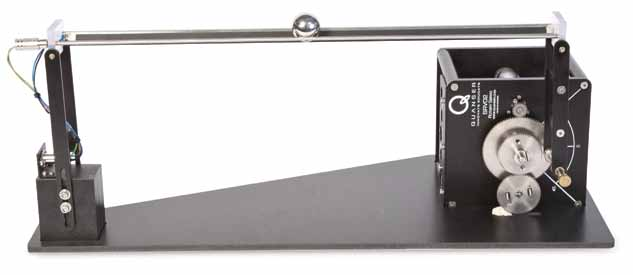
\includegraphics[width=0.5\textwidth]{quanser_ball_beam}
	\caption{Zdjęcie produktu \textit{Ball and Beam} firmy Quanser. Źródło: \url{http://www.quanser.com/Products/ball_beam}.}
	\label{fig:quanser_ball_beam}
\end{figure}

%%%%%%%%
\section{Projekt mechaniczny}

Przed przystąpieniem do budowy obiektu, zaprojektowano wstępny kształt w programie  \texttt{SketchUp Make} (\cref{fig:cad_render_1}). Wyszczególniono na nim:

\begin{itemize}
	\item prostokątną podstawę,
	\item słupy podtrzymujące belkę,
	\item usztywniający łącznik między słupami,
	\item oś obrotu (wał) umieszczony w połowie długości belki,
	\item przekrój belki.
\end{itemize}

\begin{figure}[H]
	\centering
	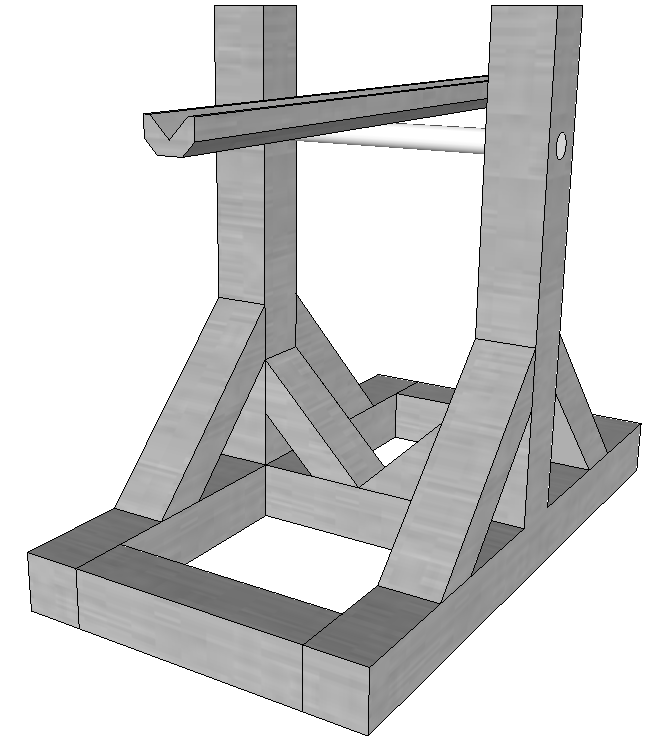
\includegraphics[width=0.4\textwidth]{cad}
	\caption{Render projektu CAD.}
	\label{fig:cad_render_1}
\end{figure}

Ostateczna konstrukcja różni się względem projektu \textsc{CAD} o wysokość słupów, i umiejscowienie łącznika między nimi. Dodatkowo zastosowano sztywne połączenie osi obrotu belki i samej belki wykorzystujące podpory wału.

%%%%%%%%
\section{Konstrukcja mechaniczna}

Większość konstrukcji powstała z ocynkowanych elementów stalowych, tzw. ceowników w przekroju kwadratowym o boku długości \SI{4}{cm}, pozwalających na łatwe łączenie kilku elementów przy pomocy śrub. Rozwiązanie to jest bardzo tanie w porównaniu do przemysłowych profili aluminiowych lub spawanych profili stalowych, ale jednocześnie jest dość ciężkie i poprzez niedomknięcie profilu podatne na pewne momenty gnące.

Kąty proste pomiędzy elementami ustawionymi prostopadle zostały zapewnione poprzez zastosowanie kątowych wsporników stalowych.

\begin{figure}[H]
	\centering
	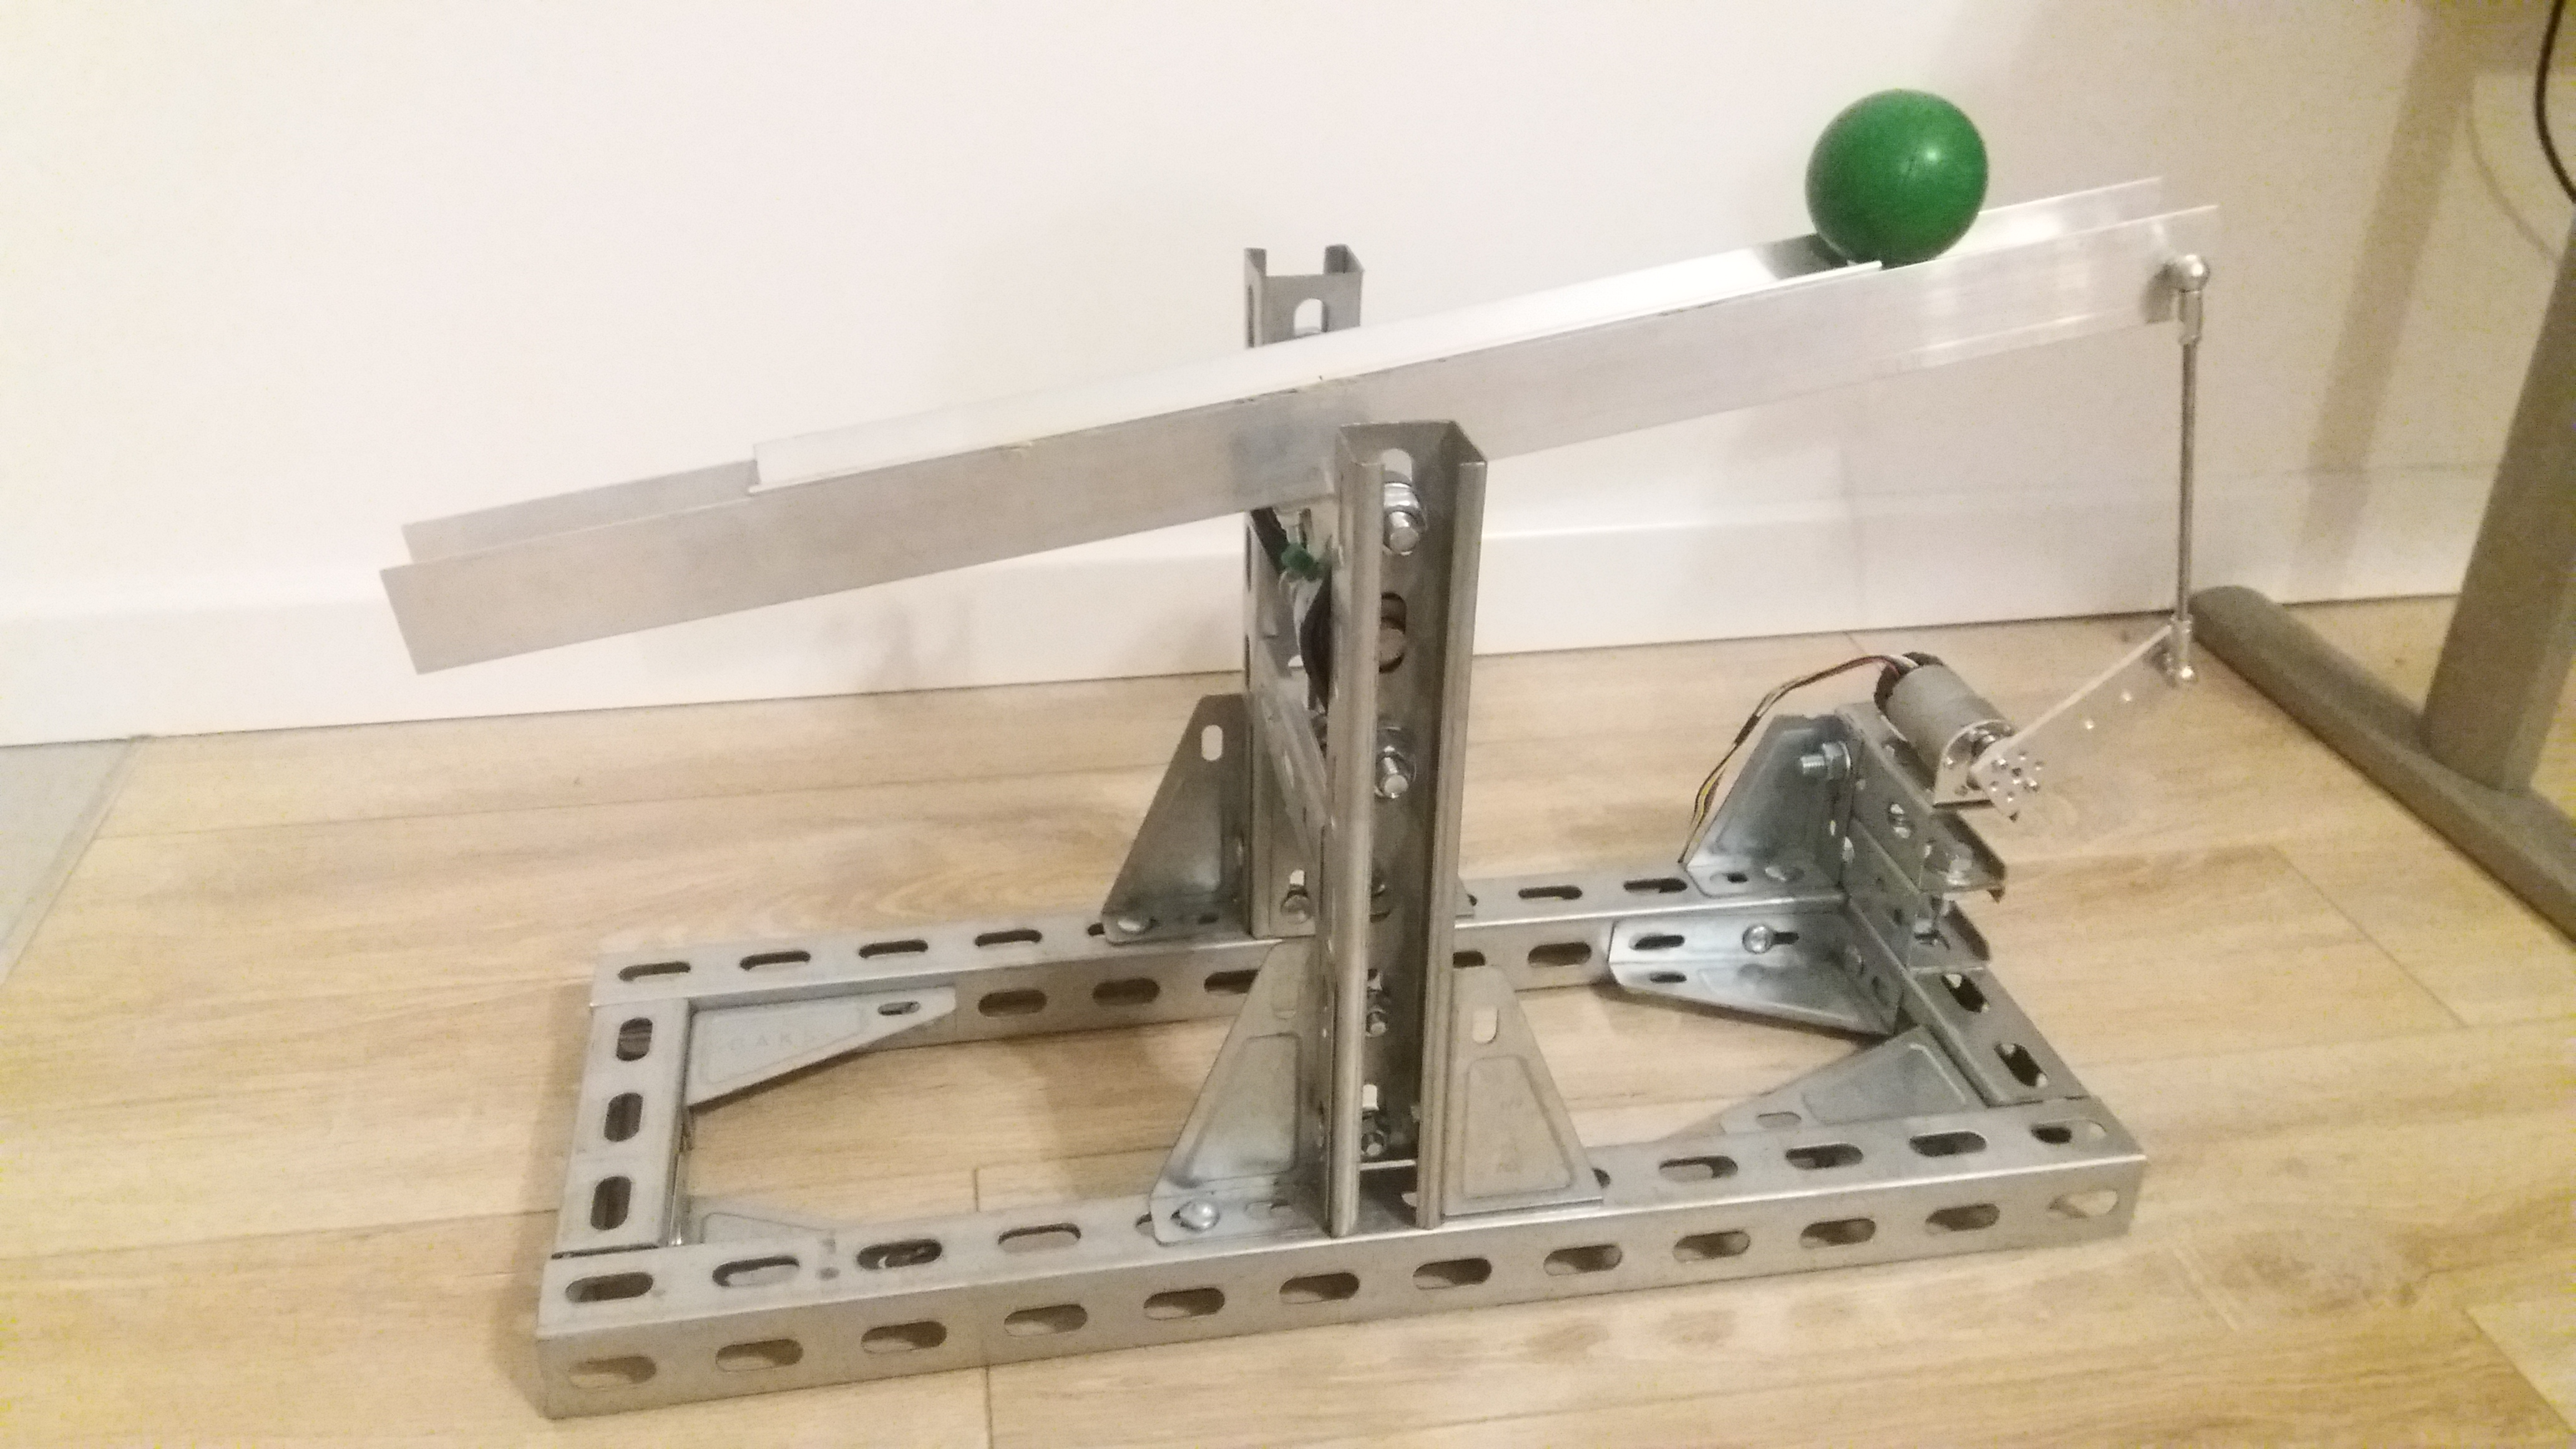
\includegraphics[width=0.7\textwidth]{mechatronics_perspective_1}
	\caption{Zdjęcie obiektu regulacji w trakcie budowy.}
	\label{fig:mechatronics_perspective_1}
\end{figure}

Na prostokątnej podstawie o wymiarach zewnętrznych \SI{60 x 23}{cm} wykonanej z ceowników ustawiono pionowo na środkach dłuższych boków słupy nośne, również wykonane z ceowników. Słupy zostały usztywnione poprzez połączenie ich przęsłem podniesionym o \SI{11}{cm} względem podstawy.

Na słupach przyczepiono współosiowo łożyska maszynowe samonastawne typu UCFL 201 w obudowach odlewanych. Przez łożyska poprowadzono pręt nierdzewny stalowy o średnicy \SI{12}{mm}; na pręt nałożono podpory wałka w kształcie litery \texttt{T}, a do nich przykręcono belkę.

Silnik elektryczny, przymocowany do aluminiowego uchwytu, został umieszczony podłużnie na krótszym boku podstawy, na podwyższeniu wykonanym z dwóch elementów stalowych typu ceownik.

% TODO: podwyższenie zostało wzmocnione przeciwko gięciom poprzecznym i wzdłużnym poprzez zastosowanie …………

%%%%%%%%
\section{Przeniesienie napędu}
\label{sec:ch2_przeniesienie_napedu}

W obiekcie zastosowano przeniesienie napędu wykorzystujące mechanizm korbowy. Rozwiązanie to posiada kilka zalet:

\begin{itemize}
	\item gwarantuje bezpieczeństwo mechanizmu -- błąd algorytmiczny (np. przypadkowe podanie maksymalnego sterowania) nie spowoduje uszkodzenia fizycznego żadnej części obiektu,
	\item poprzez oddalenie punktu zaczepu korbowodu od osi obrotu belki zmniejsza wymagania dotyczące mocy silnika, a tym samym jego cenę,
	\item pozwala regulować zakres wychyleń belki w wyniku zmiany długości korby.
\end{itemize}

% TODO: "Strzałka pokazująca silnik powinna chyba kończyć się w przegubie. Może współśrodkowo z przegubem dorysować orkąd symbolizujący silnik?"
\begin{figure}[H]
	\centering
    % TODO: przerobić rysunek w Inkscape
	% \includesvg[width=0.5\textwidth,svgpath=./graphics/]{schemat_korba}
    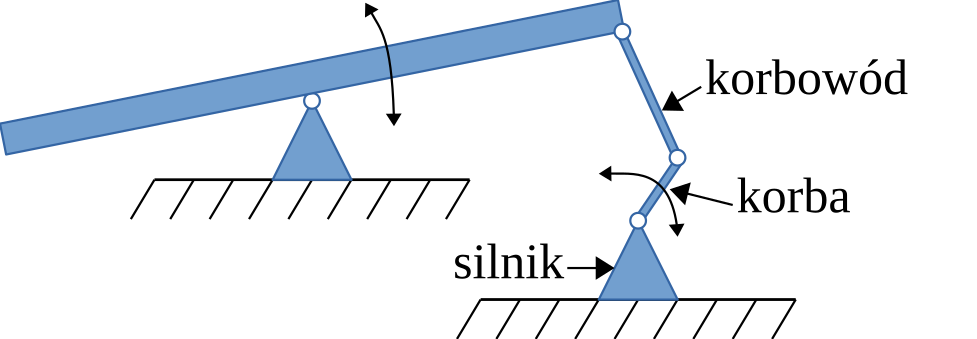
\includegraphics[width=0.5\textwidth]{schemat_korba}
	\caption{Schemat napędu opartego o mechanizm korbowy.}
	\label{fig:schemat_korba}
\end{figure}

Parametry fizyczne mechanizmu korbowego:

\begin{itemize}
	\item długość korby: \SI{3}{cm},
	\item długość korbowodu: \SI{16}{cm},
	\item zastosowane przeguby kulowe między korbą i korbowodem oraz korbowodem i belką,
    \item użyty silnik prądu stałego, komutatorowy, z magnesami trwałymi, sprzężony z zębatą przekładnią redukcyjną (więcej w rozdziale \ref{sec:ch3_uklad_napedowy}).
\end{itemize}

%%%%%%%%

\section{Belka}

Belka została stworzona poprzez trwałe sklejenie krawędzi kątownika aluminiowego o długości \SI{40}{cm} i boku \SI{3}{cm} oraz krawędzi ceownika aluminiowego o długości \SI{65}{cm} i boku \SI{4}{cm}. W przekroju przypomina to kształtem literę \texttt{M} domkniętą od spodu (\cref{fig:przekroj_belki}).

\begin{figure}[H]
	\centering
    % TODO: przerobić rysunek w Inkscape
	% \includesvg[width=0.2\textwidth,svgpath=./graphics/]{beam_xsection}
    
\includegraphics[width=0.2\textwidth]{beam_xsection}
	\caption{Schemat przekroju belki z zaznaczonymi ceownikiem aluminiowym i kątownikiem aluminiowym.}
	\label{fig:przekroj_belki}
\end{figure}

Użyty kątownik jest nieco krótszy od ceownika. Zamocowano go symetrycznie, a w odległościach około \SI{1}{cm} od jego końców zamontowano uchwyty (\cref{fig:uchwyt_czujnika_odleglosci}) na czujniki optyczne (zob. rozdział \ref{sec:ch3_czujniki_odleglosci}).

Uchwyty pozwalają na zmianę wysokości czujnika względem płaszczyzny belki, a także na pochylenie go w osi prostopadłej do płaszczyzny belki.

\begin{figure}[H]
    \centering
    % TODO: przerobić rysunek w Inkscape
    \includesvg[width=0.4\textwidth,svgpath=./graphics/]{sensor_bracket}
    \caption{Schemat uchwytu na czujnik odległości w rzucie od przodu i z boku. Zastosowanie mocowania na śrubie pozwala pochylać czujnik względem belki.}
    \label{fig:uchwyt_czujnika_odleglosci}
\end{figure}

%%%%%%%%
\section{Kulka}

Do projektu dobrano lekką kulkę o masie \SI{20}{g} wykonaną z miękkiej gąbki; średnica kulki wynosi \SI{6}{cm}.

\begin{figure}[H]
    \centering
    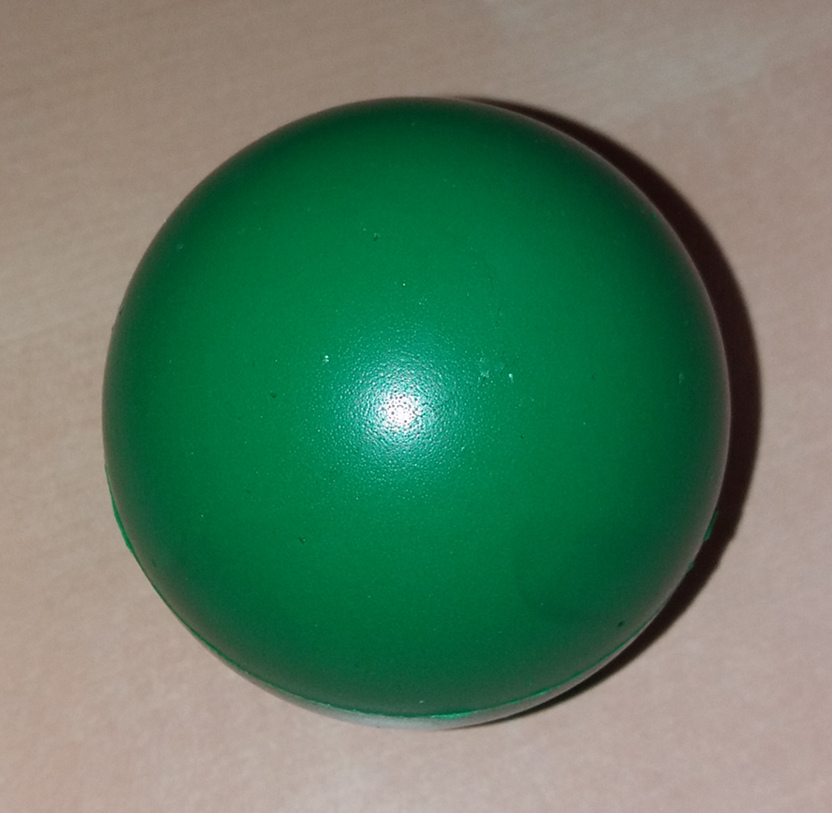
\includegraphics[width=0.4\textwidth]{ball}
    \caption{Zdjęcie kulki.}
    \label{fig:kulka}
\end{figure}

%%%%%%%%
\section{Podsumowanie}

W ninejszym rozdziale przedstawiono obiekt regulacji, cel regulacji oraz przedstawiono podobne konstrukcje, w tym jedno rozwiązanie komercyjne. Następnie opisano dokładnie budowę obiektu regulacji, poczynając od konstrukcji podstawy, poprzez umocowanie osi obrotu belki, umieszczenie silnika, przeniesienie napędu, a na budowie belki i doborze kulki kończąc.

%---------------------------------------------------------------------------
\chapter{Układ sterowania i instrumentacji}
\label{cha:ch3_uklad_ster_i_instrumentacji}

Do odczytywania danych z obiektu i sterowania nim wykorzystano opisany w tym rozdziale układ sterowania i instrumentacji (\cref{fig:schemat_ukl_sterowania_instrumentacji}). W jego sercu znajduje się przemysłowy sterownik PLC, który odczytuje dane o położeniu kulki z dwóch czujników odległości oraz położenie kątowe wału silnika z~enkodera. Dodatkowo do sterownika podłączony został czujnik bazowania oraz przyciski: \texttt{START} (NO), \texttt{STOP} (NC). Na wyjścia sterownika podłączony został mostek H kontrolujący silnik oraz dioda sygnalizacyjna.

\begin{figure}[H]
    \centering
    \includesvg[width=\textwidth,svgpath=./vector_graphics/]{uklad_sterowania_i_instrumentacji}
    % 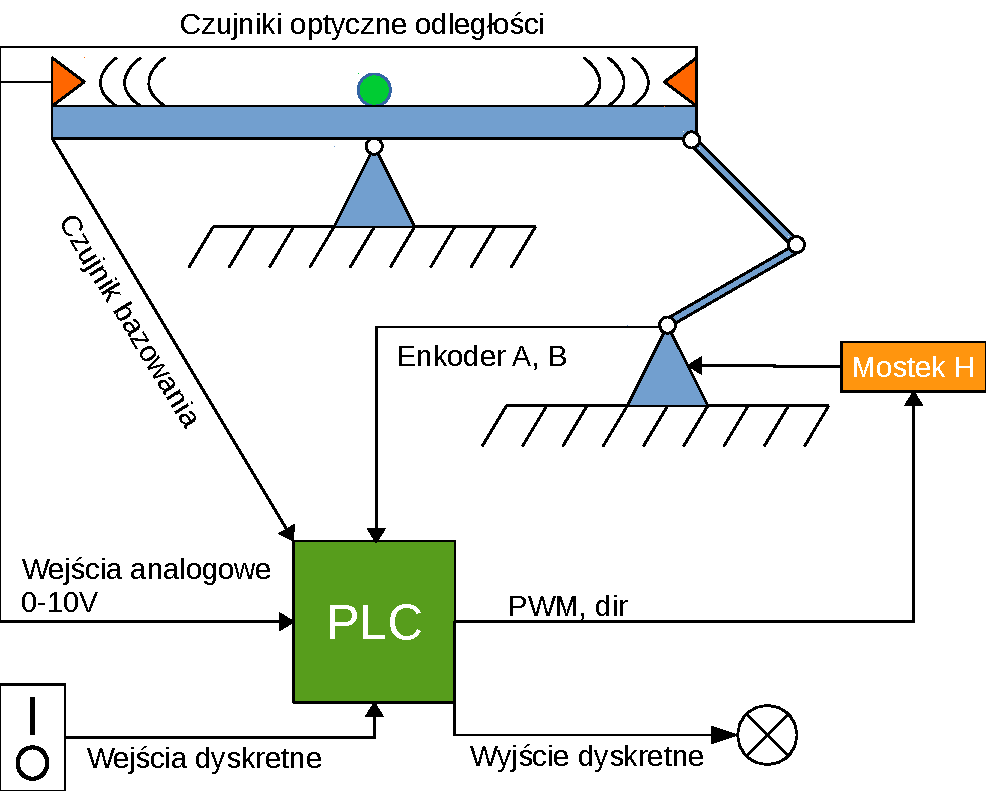
\includegraphics[width=0.7\textwidth]{schemat_ukladu3}
    \caption{Schemat układu sterowania i instrumentacji wraz z zaznaczonymi połączeniami.}
    \label{fig:schemat_ukl_sterowania_instrumentacji}
\end{figure}

%%%%%%%%
\section{Sterownik PLC}
\label{sec:ch3_PLC}

Wykorzystany w pracy sterownik PLC to \textsc{Simatic S7-1211C DC/DC/DC} firmy Siemens. Działa on na napięciu stałym \SI{24}{V}, posiada 6 wejść dyskretnych \SI{24}{V}, 4 tranzystorowe wyjścia dyskretne \SI{24}{V} i 2 napięciowe wejścia analogowe \SIrange{0}{10}{V}.

W celu ułatwienia komunikacji między sterownikiem i elektroniką opartą o logikę \SI{5}{V} (więcej w~rozdziale \ref{sec:ch3_systemy_napiec}), został on rozszerzony o dodatkową płytkę sygnałową SB 1223 działającą na logice \SI{5}{V}; dodaje ona po 2 wejścia i~wyjścia dyskretne \SI{5}{V}. Sterownik z już zamontowaną płytką przedstawiono na \cref{fig:sterownik_plytka_sygn}.

Podstawowe parametry sterownika oraz płytki sygnałowej zostały zebrane w tabeli \ref{tab:parametry_PLC_SB}:

\begin{table}[H]
    \centering
    \begin{threeparttable}
        \caption{Podstawowe parametry sterownika PLC Siemens S7-1211C i płytki sygnałowej Siemens SB 1223\tnote{a}.}
        \label{tab:parametry_PLC_SB}
        
        \begin{tabularx}{\textwidth}{p{5cm} | p{5cm} | p{5cm} }
            \toprule
            Nazwa & Siemens S7-1211C & Siemens SB 1223 \\
            \midrule
            Napięcie zasilania & \SI{24}{V} DC & \SI{5}{V} DC \\
            \midrule
            Liczba wejść cyfrowych & 6 & 2 \\
            Liczba wyjść cyfrowych & 4 & 2 \\
            Liczba wejść analogowych & 2 & 0 \\
            Liczba wyjść analogowych & 0 & 0 \\
            Typ wejść cyfrowych & \textit{sink-source} & \textit{source} \\
            Typ wyjść cyfrowych & półprzewodnikowe MOSFET \textit{source} & półprzewodnikowe MOSFET \textit{sink-source} \\
            Typ wejść analogowych & Napięciowe \SIrange{0}{10}{V} & n.d. \\
            \midrule
            Szybkie liczniki & Do 6 z częstotliwością \SI{100}{kHz}\tnote{b} & Do 2 z częstotliwością \SI{200}{kHz}\tnote{c} \\
            Wyjścia impulsowe & Do 4 z częstotliwością \SI{100}{kHz} & Do 2 z częstotliwością \SI{200}{kHz} \\
            \midrule
            Pamięć robocza & \SI{30}{kB} & n.d. \\
            Pamięć ładowania & \SI{1}{MB} & n.d. \\
            Pamięć trwała & \SI{10}{kB} & n.d. \\
            \midrule
            Czas wykonywania instrukcji boolowskich & \SI{0,08}{\micro\second}/instrukcję & n.d. \\
            Czas wykonywania operacji na typie WORD & \SI{1,7}{\micro\second}/instrukcję & n.d. \\
            Czas wykonywania operacji na typie REAL & \SI{2,3}{\micro\second}/instrukcję & n.d. \\
            \bottomrule
        \end{tabularx}
        
        \begin{tablenotes}
            \footnotesize
            \item[a] opracowanie własne na podstawie \cite{S7MANUAL},
            \item[b] w trybie kwadraturowym wykorzystywane są dwa wejścia, a~maksymalna częstotliwość wynosi \SI{80}{kHz},
            \item[c] w trybie kwadraturowym wykorzystywane są dwa wejścia, a~maksymalna częstotliwość wynosi \SI{160}{kHz}.
        \end{tablenotes}
    \end{threeparttable}
\end{table}

\begin{figure}[h]
    \centering
    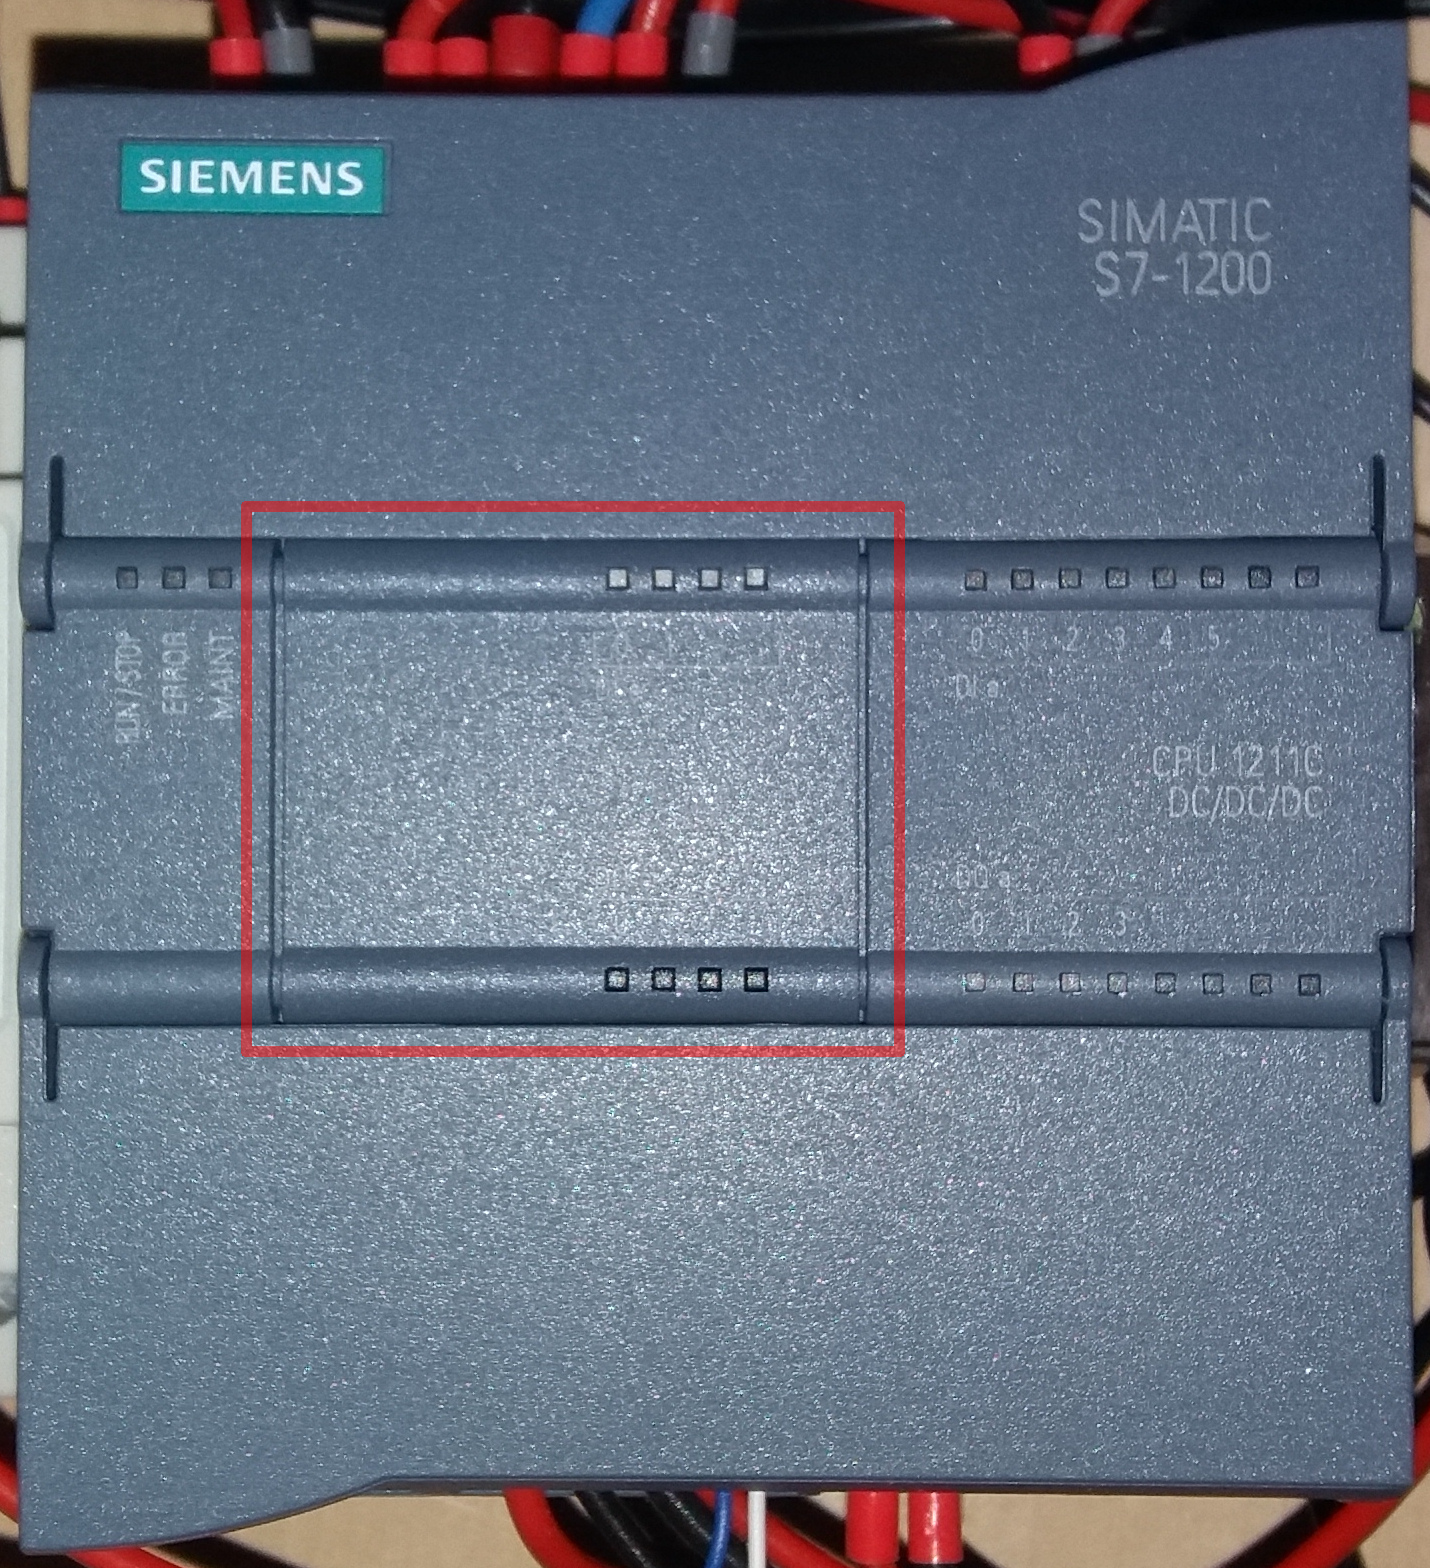
\includegraphics[width=0.5\textwidth]{s71200_sb1223}
    \caption{Zdjęcie użytego sterownika z zaznaczoną płytką sygnałową.}
    \label{fig:sterownik_plytka_sygn}
\end{figure}

%%%%%%%%
\section{Silnik z reduktorem i enkoderem}
\label{sec:ch3_uklad_napedowy}

Jak już zasygnalizowano w rozdziale \ref{sec:ch2_przeniesienie_napedu}, w pracy użyto silnik prądu stałego (komutatorowy, z~magnesami trwałymi). Silnik sprzężony jest z~zębatą przekładnią redukcyjną o przełożeniu \num{18,75}:\num{1}. Na wale silnika zamocowany jest enkoder inkrementalny kwadraturowy o~64 impulsach na obrót wału, co daje 1200 impulsów za przekładnią. Zdjęcie silnika przedstawiono na \cref{fig:silnik}.

Wybrany silnik stanowi dobry kompromis między złożonością, wydajnością i ceną. Dyskusja na temat możliwości zastosowania innych typów napędów została przeprowadzona w dodatku \ref{appA_warianty_zespolu_napedowego}.

\begin{figure}[h]
    \centering
    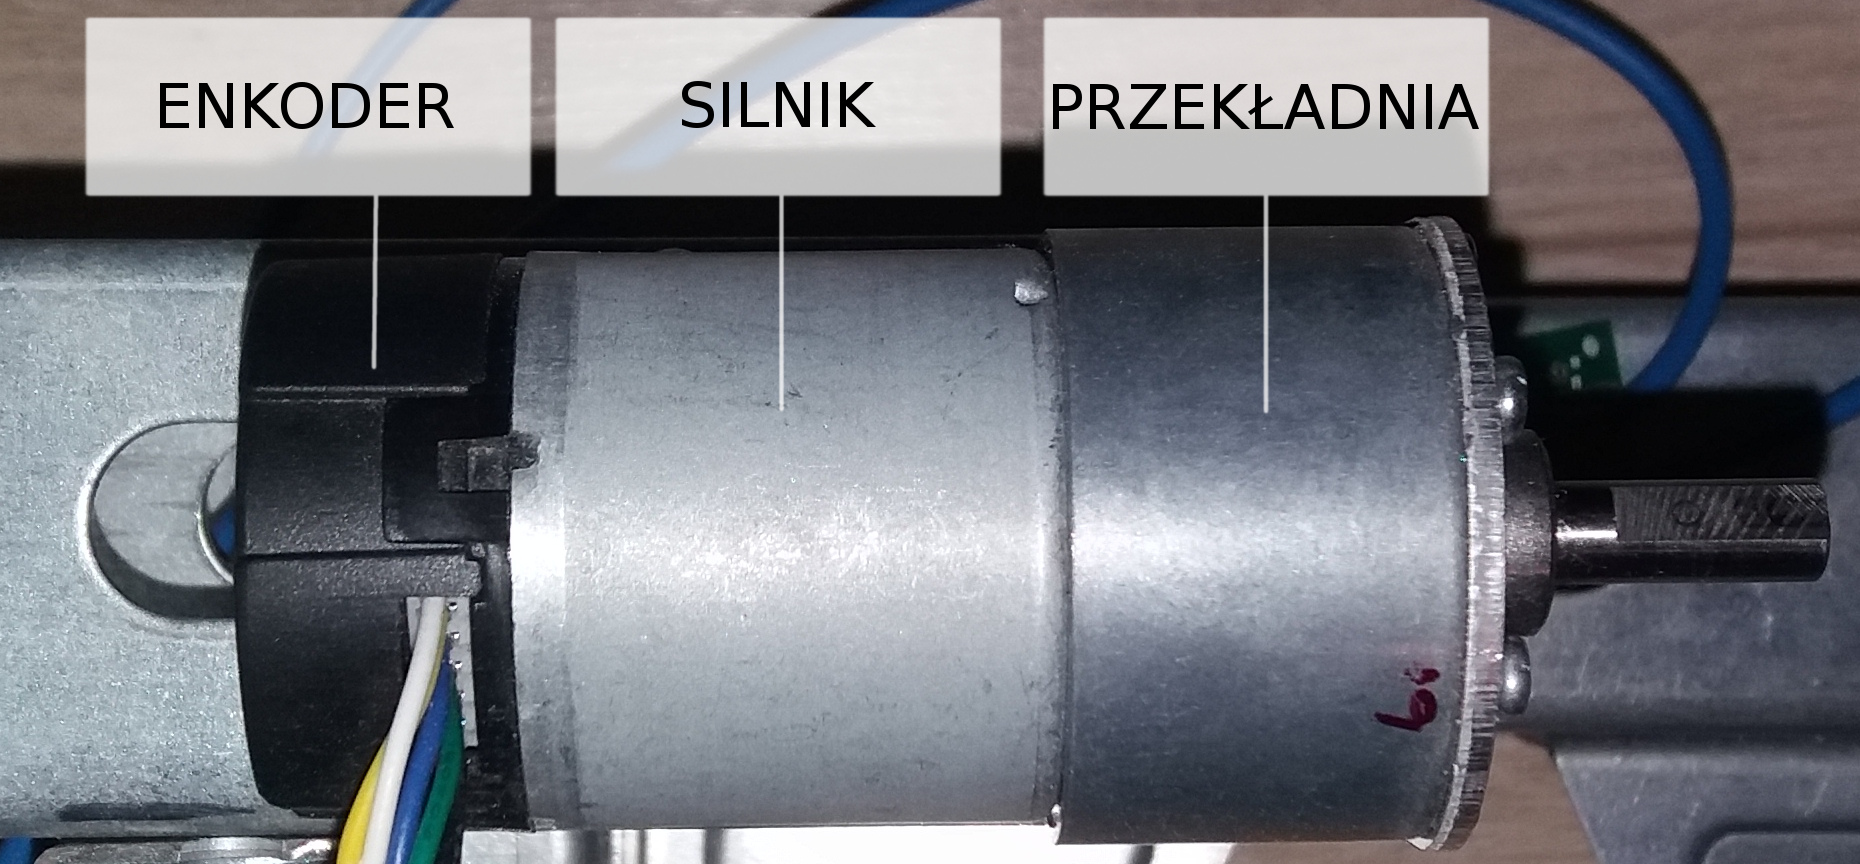
\includegraphics[width=0.55\textwidth]{silnik}
    \caption{Zdjęcie silnika w rzucie od góry z zaznaczoną przekładnią oraz enkoderem.}
    \label{fig:silnik}
\end{figure}

Producent silnika nie dostarcza pełnej dokumentacji, a jedynie kilka wybranych parametrów. Wymusiło to analityczne lub eksperymentalne wyznaczenie pozostałych wymaganych do zamodelowania silnika parametrów. Wszystkie podane parametry zostały przedstawione w tabeli \ref{tab:parametry_silnika} poniżej.

\begin{table}[H]
    \centering
    \begin{threeparttable}
        \caption{Parametry producenta silnika\tnote{a}, enkodera i przekładni\tnote{b}.}
        \label{tab:parametry_silnika}
        
        \begin{tabularx}{0.9\textwidth}{l | l}
            \toprule
            Parametr & Wartość \\
            \midrule
            Średnica & \SI{37}{\milli\meter} \\
            Długość & \SI{68}{\milli\meter} \\
            Masa & \SI{215}{g} \\
            Średnica wału & \SI{6}{\milli\meter} \\
            \midrule
            Przełożenie przekładni & \num{18,75}:\num{1} \\
            \midrule
            Napięcie znamionowe & \SI{12}{\volt} \\
            Prędkość biegu jałowego & \SI{52,36}{\radian\per\second} \\
            Prąd biegu jałowego & \SI{300}{\milli\ampere} \\
            Prąd zatrzymania silnika & \SI{5000}{\milli\ampere} \\
            Moment zatrzymania silnika & \SI{0,59}{\newton\meter} \\
            \midrule
            Typ enkodera & Kwadraturowy, inkrementalny, bez pamięci \\
            Liczba impulsów na obrót za przekładnią & \num{1200} (tryb kwadraturowy) \\
            \bottomrule
        \end{tabularx}
        
        \begin{tablenotes}
            \footnotesize
            \item[a] niektóre parametry silnika w rzeczywistości mają inne wartości, zob. rozdział \ref{sec:ch5_identyfikacja_parametrow_silnika},
            \item[b] opracowanie własne na podstawie \cite{SILNIK_MANUAL}.
        \end{tablenotes}
    \end{threeparttable}
\end{table}

Parametry niewymienione w tabeli \ref{tab:parametry_silnika}, takie jak rezystancja silnika, stała silnika, moment bezwładności wału czy współczynniki tarcia suchego i wiskotycznego, nie zostały podane przez producenta, dlatego została przeprowadzona ich identyfikacja opisana w rozdziale \ref{sec:ch5_identyfikacja_parametrow_silnika}.

Silnik sterowany jest przez PLC za pomocą układu scalonego mostka H z~tranzystorami MOSFET (Pololu BD65496MUV). Został on dobrany tak, by spełniać wymagania elektryczne silnika przy pracy znamionowej. Sterowany jest sygnałem PWM o częstotliwości \SI{20}{\kilo\hertz}. Dodatkowym sygnałem jest binarny sygnał kierunku obrotu silnika. Najistotniejsze parametry wybranego mostka H przedstawiono w~tabeli \ref{tab:parametry_mostka_H}.

\begin{table}[H]
    \centering
    \begin{threeparttable}
        \caption{Najważniejsze parametry mostka H\tnote{a}.}
        \label{tab:parametry_mostka_H}
        
        \begin{tabularx}{0.7\textwidth}{l | l}
            \toprule
            Parametr & Wartość \\
            \midrule
            Napięcie pracy silnika & \SIrange{2}{16}{\volt} \\
            Maksymalny prąd ciągły silnika & \SI{1,2}{\ampere} \\
            Maksymalny prąd chwilowy silnika & \SI{5}{\ampere} \\
            Maksymalna częstotliwość PWM & \SI{500}{\kilo\hertz} \\
            Napięcie zasilania & \SIrange{2,5}{5,5}{\volt} \\
            Napięcie sygnałów logicznych & Napięcie zasilania \SI{+-0,3}{\volt} \\
            \bottomrule
        \end{tabularx}
        
        \begin{tablenotes}
            \footnotesize
            \item[a] opracowanie własne na podstawie \cite{MOSTEK_H_MANUAL}.
        \end{tablenotes}
    \end{threeparttable}
\end{table}

Wszystkie wymagane połączenia elektryczne wykonano na uniwersalnej płytce PCB, na której umieszczono niezbędne złącza i listwy zaciskowe. Do tej samej płytki wlutowano również wspomniany mostek H, którego zdjęcie przedstawiono na \cref{fig:zdjecie_mostka_H}, a opis złącz w tabeli \ref{tab:zlacza_mostka_H}. Zdjęcie płytki PCB przedstawiono na \cref{fig:mostek_H_PCB}.

\begin{figure}[h]
    \centering
    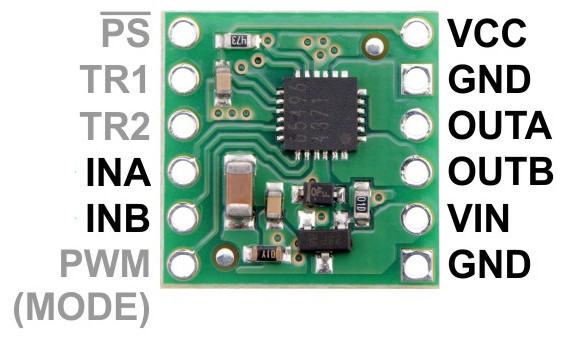
\includegraphics[width=0.4\textwidth]{mostek_H}
    \caption{Zdjęcie układu mostka H (Pololu BD65496MUV). Źródło: \url{https://www.pololu.com/product/2960}.}
    \label{fig:zdjecie_mostka_H}
\end{figure}

\begin{table}[H]
    \centering
    \begin{threeparttable}
        \caption{Opis złącz mostka H\tnote{a}.}
        \label{tab:zlacza_mostka_H}
        
        \begin{tabularx}{0.67\textwidth}{l | l}
            \toprule
            Złącze & Opis \\
            \midrule
            \texttt{VCC} & Zasilanie układu \\
            \texttt{VIN} & Zasilanie silnika \\
            \texttt{GND} & Masa \\
            \texttt{OUTA}, \texttt{OUTB} & Wyjścia zasilania silnika \\
            \texttt{INA}, \texttt{INB} & Wejścia sygnałów sterujących \\
            \texttt{PWM (MODE)} & Przełączanie między trybem \texttt{IN/IN} a~\texttt{EN/IN}\tnote{b} \\
            \texttt{PS} & Oszczędzanie energii \\
            \texttt{TR1}, \texttt{TR2} & Kontrola maksymalnej częstotliwości \\
            \bottomrule
        \end{tabularx}
        
        \begin{tablenotes}
            \footnotesize
            \item[a] opracowanie własne na podstawie \cite{MOSTEK_H_MANUAL},
            \item[b] układ umożliwia sterowanie silnikiem w trybie \texttt{IN/IN} oraz \texttt{EN/IN}; ten pierwszy przekazuje sygnał wysoki ze złącza \texttt{INA} na \texttt{OUTA} i \texttt{INB} na \texttt{OUTB} (za wyjątkiem sytuacji dwóch stanów wysokich), natomiast ten drugi pozwala użyć sygnału PWM (\texttt{INA}) oraz sygnału kierunku obrotu (\texttt{INB}).
        \end{tablenotes}
    \end{threeparttable}
\end{table}

W układzie nie zastosowano czujnika położenia wału, do którego przymocowana jest belka; zamiast tego wykorzystano zależność geometryczną pomiędzy obrotem wału silnika a obrotem belki. W przypadku niewielkich odchyleń kąt belki $\theta$ powinien być liniowo związany z kątem obrotu wału silnika $\alpha$~w~następujący sposób:

\begin{equation}\label{eq:uproszczona_zaleznosc_kata_belki}
    \theta = \frac{L}{d_k} \alpha
\end{equation}
gdzie: $L$ to odległość końca belki od osi obrotu, $d_k$ to długość korby. Zależność \eqref{eq:uproszczona_zaleznosc_kata_belki} wynika z założenia, że punkty zaczepu korbowodu przebędą taką samą drogę łukową, a zatem $\theta d_k = \alpha L$.

Niestety, równanie \eqref{eq:uproszczona_zaleznosc_kata_belki} jest poprawne tylko w niewielkich odchyleniach belki od poziomu oraz gdy linia łącząca punkt zaczepu mechanizmu korbowego i oś obrotu belki jest równoległa do korby. Faktyczna zależność $\theta(\alpha)$ została zidentyfikowana za pomocą modelu symulacyjnego (rozdział \ref{sec:ch4_zaleznosc_kata_silnika_i_kata_belki}).

\begin{figure}[H]
    \centering
    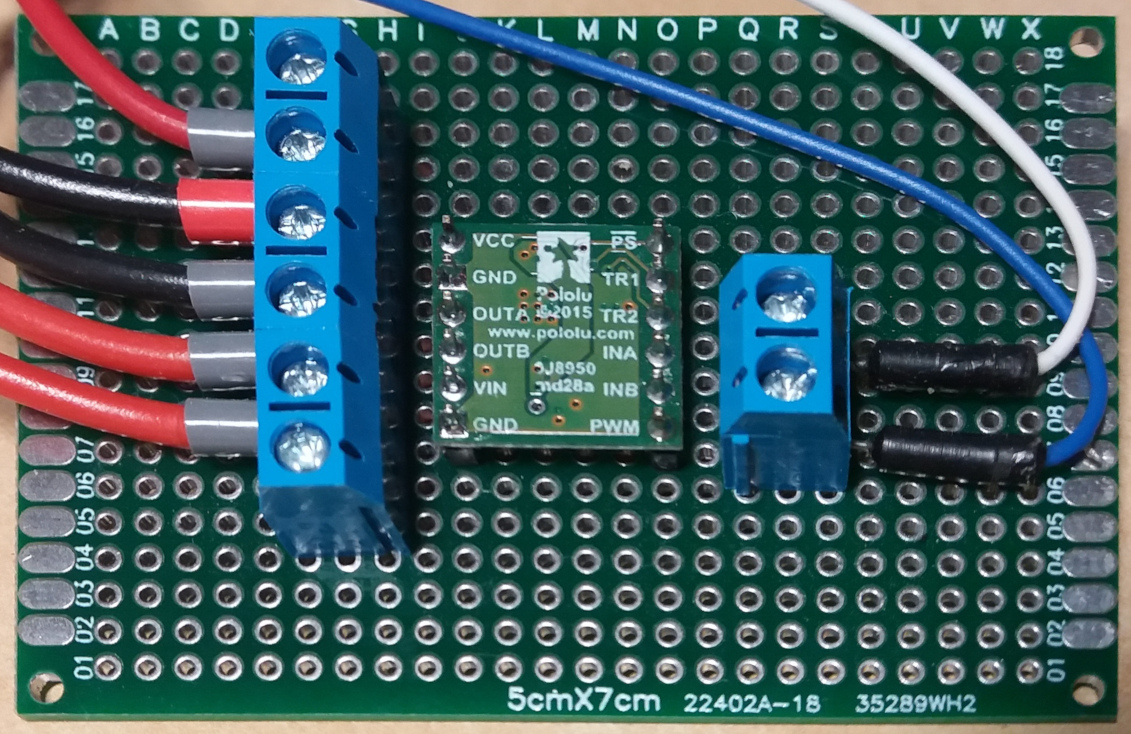
\includegraphics[width=0.6\textwidth]{mostek_H_PCB}
    \caption{Zdjęcie płytki PCB z zamontowanym układem mostka H (Pololu BD65496MUV).}
    \label{fig:mostek_H_PCB}
\end{figure}

%%%%%%%%
\section{Czujniki odległości}
\label{sec:ch3_czujniki_odleglosci}

Do pomiaru położenia kulki wykorzystano parę analogowych czujników Sharp GP2Y0A41SK0F (\cref{fig:czujnik_sharp}). Każdy z czujników składa się z nadajnika światła podczerwonego i odbiornika; obliczanie pozycji obiektu odbywa się na zasadzie triangulacji. Podstawowe parametry czujników opisano w tabeli \ref{tab:parametry_czujnikow_Sharp}.

\begin{figure}[h]
    \centering
    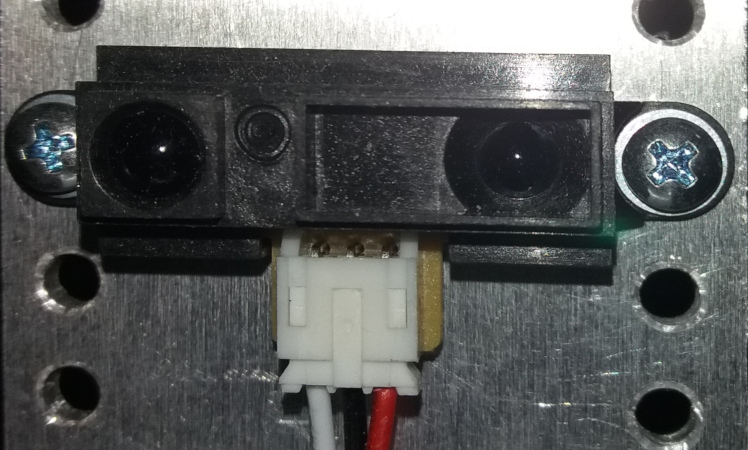
\includegraphics[width=0.5\textwidth]{czujnik}
    \caption{Zdjęcie czujnika Sharp GP2Y0A41SK0F.}
    \label{fig:czujnik_sharp}
\end{figure}

Czujniki optyczne pracujące w podczerwieni nie są jedynymi sensorami, które można zastosować do badania położenia kulki w układach typu kulka i belka. Alternatywne sposoby zostały omówione w~dodatku \ref{appB_alternatywne_czujniki_pozycji_kulki}.

\begin{table}[h]
    \centering
    \begin{threeparttable}
        \caption{Podstawowe parametry czujników pozycji kulki\tnote{a}.}
        \label{tab:parametry_czujnikow_Sharp}
        
        \begin{tabularx}{0.75\textwidth}{l | l}
            \toprule
            Parametr & Wartość \\
            \midrule
            Napięcie zasilania & \SIrange{4,5}{5,5}{\volt} \\
            Zakres pomiarowy & \SIrange{4}{30}{\centi\meter} \\
            Typ sygnału wyjściowego & Analogowy napięciowy około \SIrange{0,25}{3,1}{\volt} \\
            \bottomrule
        \end{tabularx}
        
        \begin{tablenotes}
            \footnotesize
            \item[a] opracowanie własne na podstawie \cite{SHARP_MANUAL}.
        \end{tablenotes}
    \end{threeparttable}
\end{table}

Czujniki zostały zamontowane na wspornikach umożliwiających regulację wysokości oraz pochylenia względem belki (zob. rozdział \ref{sec:ch2_belka}). Odległość między czujnikami to \SI{40}{\centi\meter} (powyżej górnej granicy zakresu pomiarowego), a ich wysokość nad belką to \SI{4}{\centi\meter}. W dalszej części pracy, czujnik zamontowany dalej od punktu zaczepu korbowodu nazywany jest ,,lewy'', natomiast czujnik zamontowany bliżej tego punktu --- ,,prawy''.

Charakterystyka każdego z czujników jest mocno nieliniowa (zob. \cref{fig:charakterystyka_czujnikow}). Dobrą aproksymację charakterystyki można otrzymać (po odcięciu wartości poniżej \SI{3}{\centi\meter}) za pomocą funkcji postaci $y =\nobreak a x ^ b + c$ (zob. tabela \ref{tab:aproksymacja_czujnikow}), gdzie $x$ to wartość pomiaru z przetwornika, a $y$ to odległość do przeszkody.

Sposób zebrania charakterystyk czujników oraz wykonana aproksymacja zostały opisane w rozdziale~\ref{sec:ch5_identyfikacja_charakterystyk_czujnikow}.

\begin{figure}[h]
    \centering
    \includesvg[width=\textwidth,svgpath=./vector_graphics/]{charakterystyka_czujnikow}
    \caption{Charakterystyka czujników odległości.}
    \label{fig:charakterystyka_czujnikow}
\end{figure}

Z powodu dużej złożoności obliczeniowej liczenia potęg niecałkowitych zrezygnowano z implementacji takich aproksymacji w sterowniku PLC. Wobec tych utrudnień zastosowano inne rozwiązanie w~celu obliczenia pozycji kulki: aproksymację liniową pomiędzy punktami charakterystyki. W tym celu wprowadzono punkty charakterystyki każdego z czujników (pary: wartość z przetwornika ADC, odległość do kulki) do dwóch tablic w sterowniku PLC.

Oba czujniki są równoodległe ($x_d = \SI{20}{\centi\meter}$) od środka belki, co oznacza, że aby uzyskać wychylenie środka kulki od środka belki, należy transformować układy odniesienia czujników, co ilustruje \cref{fig:polozenie_kulki}. Mając dwie odległości $d_l$ oraz $d_r$ od czujników do kulki, pozycję kulki $d_b$ oblicza się w~następujący sposób:
\begin{equation}\label{eq:pozycja_kulki}
d_b = \frac{d_l + 2\cdot d_c - d_r}{2} - d_c
\end{equation}

\begin{figure}[H]
    \centering
    \includesvg[width=0.5\textwidth,svgpath=./vector_graphics/]{pozycja_kulki}
    \caption{Położenie kulki względem środka belki i czujników.}
    \label{fig:polozenie_kulki}
\end{figure}


%%%%%%%%
\section{Czujnik bazowania}
\label{sec:ch3_czujnik_bazowania}

% TODO: uaktualnij odnośnik
Z powodu wykorzystania enkodera inkrementalnego, po każdym uruchomieniu urządzenia konieczne jest przeprowadzenie procedury bazowania (zob. rozdział \ref{cha:ch7_algorytmy_sterowania}) w celu określenia dokładnej pozycji kątowej wału silnika, a co za tym idzie: pozycji kątowej belki.

Do wykrycia pozycji bazowania wykorzystano transoptor szczelinowy TCST1103 firmy Vishay Semiconductors połączony w układzie przedstawionym na \cref{fig:uklad_transoptora}, natomiast podstawowe parametry transoptora zostały opisane w tabeli \ref{tab:parametry_transoptora}.

\begin{figure}[H]
    \centering
    \includesvg[width=0.8\textwidth,svgpath=./vector_graphics/]{uklad_transoptora}
    % 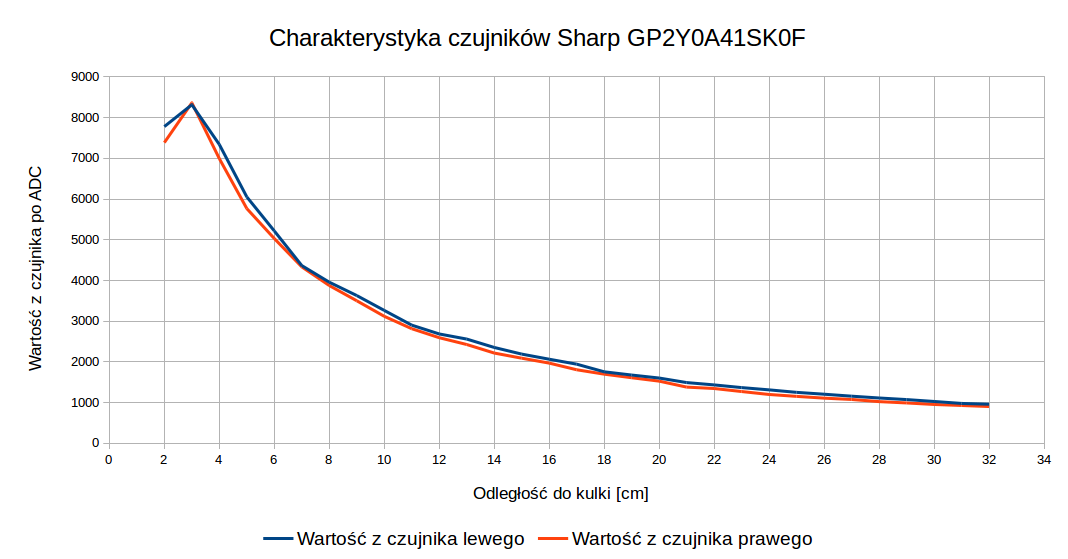
\includegraphics[width=1\textwidth]{sensor_characteristics}
    \caption{Schemat podłączenia układu transoptora.}
    \label{fig:uklad_transoptora}
\end{figure}

\begin{table}[h]
    \centering
    \begin{threeparttable}
        \caption{Podstawowe parametry transoptora szczelinowego\tnote{a}.}
        \label{tab:parametry_transoptora}
        
        \begin{tabularx}{0.6\textwidth}{l | l}
            \toprule
            Parametr & Wartość \\
            \midrule
            Szerokość szczeliny & \SI{3}{\milli\meter} \\
            Maks. natężenie przewodzenia diody & \SI{60}{\milli\ampere} \\
            Maks. napięcie kolektor-emiter & \SI{70}{\volt} \\
            Współczynnik wzmocnienia prądowego & \num{0,2} \\
            \bottomrule
        \end{tabularx}
        
        \begin{tablenotes}
            \footnotesize
            \item[a] opracowanie własne na podstawie \cite{TRANSOPTOR_MANUAL}.
        \end{tablenotes}
    \end{threeparttable}
\end{table}

Układ z \cref{fig:uklad_transoptora} przylutowano do płytki uniwersalnej (\cref{fig:czujnik_bazowania_PCB}). Elementy \texttt{J1} oraz \texttt{J2} reprezentują złącza zaciskowe, za pomocą których zrealizowano połączenia elektryczne z zasilaniem oraz sterownikiem PLC.

\begin{figure}[h]
    \centering
    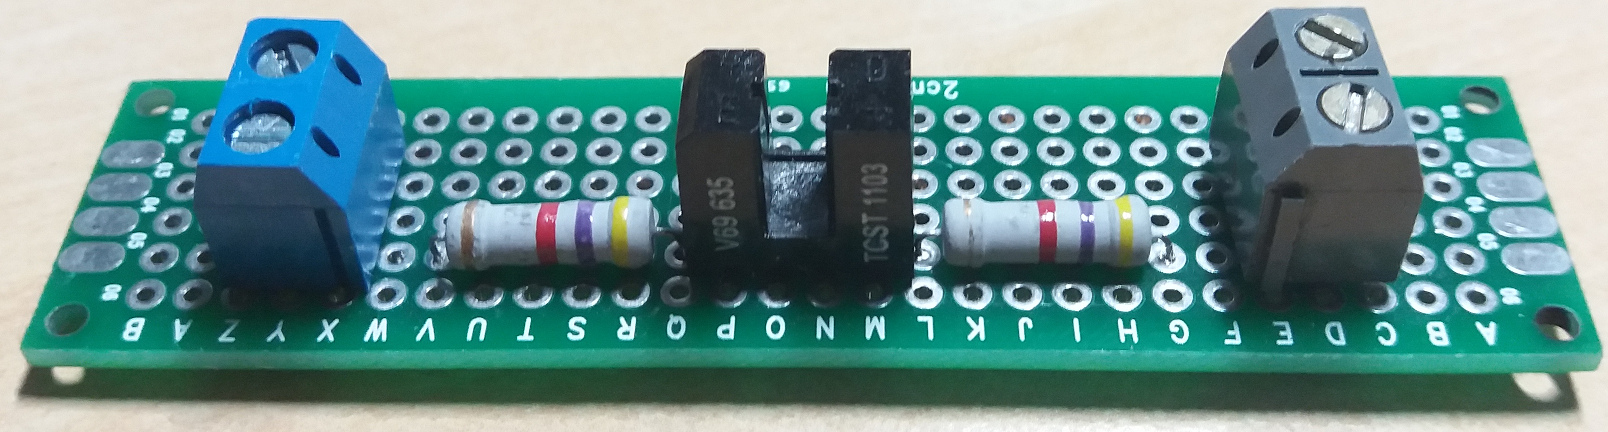
\includegraphics[width=0.6\textwidth]{czujnik_bazowania_PCB}
    \caption{Zdjęcie płytki PCB z zamontowanym układem z \cref{fig:uklad_transoptora}.}
    \label{fig:czujnik_bazowania_PCB}
\end{figure}

% TODO: zweryfikuj ilość impulsów do bazowania
Płytka z czujnikiem bazowania została przytwierdzona do układu kulki i belki poniżej silnika. Sztywny, lekki i nieprzezroczysty element przyczepiony został na końcu korby tak, aby przechodził przez szczelinę enkodera w momencie skierowania korby pionowo w dół. Przyjęto, że w chwili zasłonięcia szczeliny (przy ruchu zgodnie ze wskazówkami zegara) licznik enkodera powinien otrzymać wartość \num{75}; wówczas poziomemu położeniu belki odpowiada wartość \num{0}.

%%%%%%%%
\section{Systemy napięć}
\label{sec:ch3_systemy_napiec}

Jak można zauważyć, elementy elektroniczne i elektromechaniczne użyte do zbudowania obiektu sterowania korzystają z poziomów logicznych o różnych napięciach (\cref{tab:poziomy_napiec}). Wynika to z faktu połączenia obiektu typowo przemysłowego, jakim jest sterownik PLC Siemens S7-1211C, który wykorzystuje napięcie \SI{24}{\volt}, oraz elektroniki hobbystycznej (czujniki odległości, mostek H, enkoder), która wykorzystuje napięcia \SI{5}{\volt}. Dodatkowym utrudnieniem jest element wykonawczy, tj. silnik prądu stałego, o napięciu znamionowym 12V.

\begin{table}[h]
    \centering
    \begin{threeparttable}
        \caption{Podział modułów elektronicznych ze względu na wykorzystywany poziom napięcia.}
        \label{tab:poziomy_napiec}
        
        \begin{tabularx}{0.6\textwidth}{l | l}
            \toprule
            Element & Napięcie \\
            \midrule
            Sterownik PLC & \SI{24}{\volt} \\
            Płytka sygnałowa & \SI{5}{\volt} \\
            Mostek H (logika) & \SI{5}{\volt} \\
            Mostek H (zasilanie silnika)\tnote[a] & \SI{12}{\volt} \\
            Enkoder & \SI{5}{\volt} \\
            Czujniki odległości (zasilanie) & \SI{5}{\volt} \\
            Czujniki odległości (wyjście analogowe) & \SIrange{0,25}{3,1}{\volt} \\
            Sterownik PLC (wejścia analogowe) & \SIrange{0}{10}{\volt} \\
            Czujnik bazowania & \SI{24}{\volt} \\
            Przyciski & \SI{24}{\volt} \\
            Dioda sygnalizacyjna & \SI{24}{\volt} \\
            \bottomrule
        \end{tabularx}
        
        \begin{tablenotes}
            \footnotesize
            \item[a] wartość napięcia znamionowego silnika, zob. tab. \ref{tab:parametry_silnika}.
        \end{tablenotes}
    \end{threeparttable}
\end{table}

Obecność trzech systemów napięcia poskutkowała użyciem trzech oddzielnych zasilaczy: \SI{24}{\volt} o~mocy \SI{60}{\watt}, \SI{12}{\volt} o~mocy \SI{15}{\watt}, \SI{5}{\volt} o~mocy \SI{12,5}{\watt}. Wszystkie zasilacze zostały połączone wspólną masą.

%%%%%%%%
\section{Okablowanie i zabezpieczenia}
\label{sec:ch3_okablowanie_zabezpieczenia}

% TODO: dodaj zdjęcie "szafy"

Połączenia elektryczne pomiędzy komponentami pracy zrealizowano za pomocą przewodów o przekroju \SI{0,75}{\milli\meter\squared}. Za wyjątkiem złącza silnika i enkodera, wszystkie przewody zakończone są tulejami, co jest konieczne z powodu zastosowania złącz śrubowych.

Zasilanie po stronie \SI{230}{\volt} AC, \SI{50}{\hertz} zostało zabezpieczone instalacyjnym wyłącznikiem nadprądowym klasy B10.

% TODO: zweryfikuj ilość, rozłożenie szyn
Wyłącznik nadprądowy, zasilacz \SI{12}{\volt}, zasilacz \SI{24}{\volt} oraz sterownik PLC zostały przymocowane do wspólnej szyny DIN (TH \num{35}). Dodatkowo zamontowano na niej listwy przyłączeniowe dla każdego poziomu napięcia (zob. rozdział \ref{sec:ch3_systemy_napiec}): \SI{0}{\volt} (wspólna masa), \SI{5}{\volt}, \SI{25}{\volt}. Z napięcia \SI{12}{\volt} korzysta tylko silnik, więc to połączenie zostało zrealizowane bezpośrednio, bez użycia listwy przyłączeniowej.

Zasilacz \SI{5}{\volt} posiada jednofazową wtyczkę elektryczną bez uziemienia, dlatego na szynie DIN dodatkowo zamontowano gniazdko elektryczne połączone szeregowo z wyłącznikiem nadprądowym.

% TODO: dodaj ilustrację szyn

%%%%%%%%
\section{Podsumowanie}

W niniejszym rozdziale przedstawiono układy elektryczne, elektroniczne i elektromechaniczne wykorzystane do stworzenia obiektu typu kulka i belka. Następnie opisano poszczególnych elementów: sterownika PLC, płytki sygnałowej, silnika, enkodera, mostku H i czujników odległości. Przedstawiono charakterystyki czujników, sposób ich implementacji w sterowniku oraz sposób obliczania pozycji kulki. Następnie przedstawiono czujnik wykorzystywany do bazowania.

W kolejnych podrozdziałach poruszono kwestię różnych systemów napięć, zastosowanych zasilaczy, zabezpieczeń, okablowania i organizacji przewodów.

%---------------------------------------------------------------------------
\chapter{Model symulacyjny}
\label{cha:ch4_model_symulacyjny}

Do zaprojektowania odpowiedniego układu regulacji systemem kulka i belka, a więc dobrania struktury regulatorów, konieczne jest posiadanie modelu tego systemu. Jest to jednak zadanie utrudnione, gdy system jest wybitnie nieliniowy --- a obiekt regulacji taki właśnie jest, gdyż zawiera nieliniowości wynikające z:
\begin{itemize}
    \item przeniesienia napędu poprzez przekładnię korbową,
    \item wynikającej z tego przeniesienia zależności obrotu belki od obrotu silnika,
    \item czy z obecnego w przekładni zastosowanego silnika tarcia suchego.
%    \item dzia.
\end{itemize}

Wobec tego zdecydowano się nie przystępować do opisu matematycznego zachowania się układu w sposób klasyczny, np. poprzez równania Eulera--Lagrange'a czy funkcjonał Hamiltona. Zamiast tego, wykorzystując narzędzia pakietu \textsc{Matlab/Simulink}, zbudowano przestrzenną i fizyczną reprezentację obiektu regulacji, która następnie została wykorzystana do linearyzacji i dobrania regulatorów (rozdział \ref{cha:ch6_model_liniowy}).

\section{Wykorzystanie przybornika \textsc{Simscape Multibody}}
\label{sec:ch4_simmechanics}

\textsc{Simscape Multibody}, znany również jako \textsc{SimMechanics}, pozwala na modelowanie fizycznych układów (ciał stałych o określonej geometrii, masie i/lub inercji) oraz zależności między nimi (transformacje i rotacje pozycji). Bardzo ważną cechą jest możliwość stosowania więzów pomiędzy kilkoma układami odniesienia. Więzy te mają zero lub więcej stopni swobody i nazywane są przegubami lub złączami; do najbardziej charakterystycznych należą złącza pryzmatyczne, obrotowe czy sferyczne (zob. \cref{fig:simmechanics_bloki}). Jak można zauważyć, odpowiadają one fizycznym połączeniom ruchowym lub obrotowym spotykanym w układach mechanicznych.

Ponadto przybornik \textsc{SimMechanics} umożliwia symulowanie zachowania układu i może być zastosowany do numerycznego rozwiązywania prostego i odwrotnego zadania kinematyki i mechaniki.

\begin{figure}[h]
    \centering
    \begin{subfigure}[t]{0.2\textwidth}
        \centering
        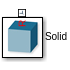
\includegraphics[width=0.75\textwidth]{sm_solid}
        \caption{Ciało stałe.}
        \label{fig:sm_solid}
    \end{subfigure}
    ~ 
    \begin{subfigure}[t]{0.2\textwidth}
        \centering
        
\includegraphics[width=0.75\textwidth]{sm_rigid_transform}
        \caption{Transformacja układu odniesienia.}
        \label{fig:sm_rigid_transform}
    \end{subfigure}
    ~ 
    \begin{subfigure}[t]{0.2\textwidth}
        \centering
        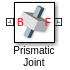
\includegraphics[width=0.75\textwidth]{sm_prismatic_joint}
        \caption{Złącze pryzmatyczne.}
        \label{fig:sm_prismatic_joint}
    \end{subfigure}
    ~
    \begin{subfigure}[t]{0.2\textwidth}
        \centering
        
\includegraphics[width=0.75\textwidth]{sm_revolute_joint}
        \caption{Złącze obrotowe.}
        \label{fig:sm_revolute_joint}
    \end{subfigure}
    
    \caption{Podstawowe bloki budujące schemat \textsc{SimMechanics}.}
    \label{fig:simmechanics_bloki}
\end{figure}

Budowanie schematu z wykorzystaniem bloków \textsc{SimMechanics} polega na, w dużym uproszczeniu, przyłączaniu ciał stałych w centrach układów odniesienia, które przemieszczane są w przestrzeni za pomocą bloków \textit{Rigid Transform} (rys. \ref{fig:sm_rigid_transform}). Wspomniane bloki umożliwiają również rotację układów odniesienia, co jest często konieczne do poprawnego działania złącz o pewnej liczbie stopni swobody. Przykładowo, złącze \textit{Revolute Joint} (\cref{fig:sm_revolute_joint}) umożliwia obracanie układu odniesienia \texttt{F} (ang. \textit{Follower} --- następujący układ odniesienia) wokół osi Z~układu \texttt{B} (ang. \textit{Base} --- poprzedzający układ odniesienia)\footnote{W ustawieniach bloku \textit{Revolute Joint} możliwa jest zmiana na tryb odwrotny, tj. obrót układu \texttt{B} wokół układu \texttt{F}.}. Jednakże jeśli wał, który ma się obracać wokół swojej naturalnej osi obrotu, nie ma w swoim układzie osi Z~wzdłuż naturalnej osi obrotu, wtedy jego układ odniesienia musi zostać transformowany za pomocą \textit{Rigid Transform}.

Bloki złącz umożliwiają pozyskanie informacji o aktualnych wartościach pozycji, prędkości i przyspieszenia (w zależności od typu złącza odpowiednio liniowych lub obrotowych) oraz przyłożonego na złącze momentu obrotowego lub siły. Dodatkowo możliwe jest załączenie wejścia momentu oddziałującego lub siły, co zostało wykorzystane przy implementacji silnika.

Ostatnią wartą wspomnienia informacją jest możliwość ustawienia pewnej wartości wstępnej dla danego złącza (warunku początkowego). W przypadku złącza \textit{Revolute Joint} umożliwia to wymuszenie kąta obrotu pomiędzy układami odniesienia \texttt{B} oraz \texttt{F}, a w przypadku złącza \textit{Prismatic Joint} wymusza to odpowiednie przesunięcie.

\section{Reprezentacja obiektu typu kulka i belka}
\label{sec:ch4_reprezentacja_obiektu_kulka_i_belka}

Bardzo dużą zaletą korzystania z \textsc{SimMechanics} jest automatyczne generowanie podglądu i animacji (zob. \cref{fig:uklad_simmechanics}) budowanego układu. Pozwala to przeprowadzać obserwację działania różnych algorytmów sterowania oraz łatwo znajdować błędy złożenia brył.

\begin{figure}[h]
    \centering
    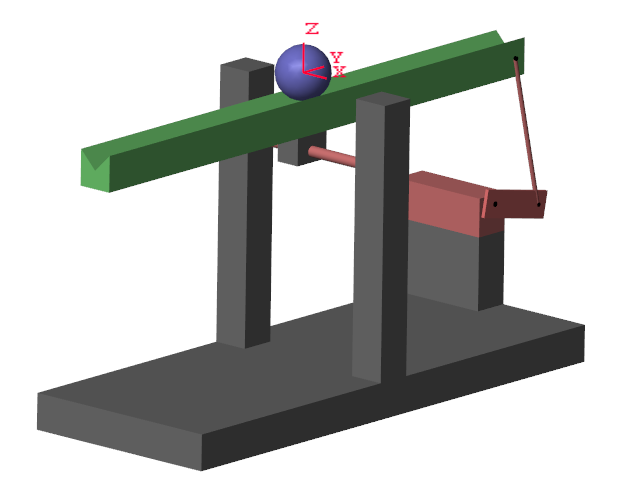
\includegraphics[width=0.5\textwidth]{simmechanics_ballandbeam}
    \caption{Wizualizacja układu kulki i belki zamodelowanego przy pomocy \textsc{SimMechanics} (por. z obiektem rzeczywistym przedstawionym na \cref{fig:perspektywa}).}
    \label{fig:uklad_simmechanics}
\end{figure}

Schemat użyty do wygenerowania modelu z \cref{fig:uklad_simmechanics} został przedstawiony na \cref{fig:uklad_simmechanics2}. Poczynając od lewej strony, możemy na nim wyróżnić kilka charakterystycznych elementów:

\begin{itemize}
    \item obiekty \textit{Base}, \textit{Tower1}, \textit{Tower2}, \textit{MotorBase}, \textit{Shaft Supports}, \textit{Motor}, \textit{Beam}, \textit{Pin2}, \textit{Ball} oraz \textit{CrankShaft},
    \item podsystemy \textit{Shaft}, \textit{Electric Motor}, \textit{Crank} oraz \textit{Ball mechanics},
    \item sporo bloków \textit{Rigid Transform} o nazwach \textit{RT}---\textit{RT19},
    \item trzy bloki \textit{Revolute Joint},
    \item wejścia \textit{voltage} oraz \textit{disturbance},
    \item wyjścia \textit{ball\_position}, \textit{ball\_velocity}, \textit{beam\_angle} oraz \textit{beam\_angular\_velocity}.
\end{itemize}

Obiekt \textit{Base} reprezentuje podstawę, na której umieszczono całą mechanikę układu. Poprzez transformacje \textit{RT} oraz \textit{RT1} umieszczono na nim dwa słupy, na których zaczepione są łożyska i wał obrotowy belki (podsystem \textit{Shaft}, \cref{fig:sm_shaft}).

Wał belki składa się z dwóch równoległych ścieżek, transformowanych z globalnego układu odniesienia poprzez bloki \textit{RT2} oraz \textit{RT3}. Za blokami umieszczono złącza obrotowe \textit{BallBearing1} oraz \textit{BallBearing2}, reprezentujące fizyczne łożyska kulkowe (zob. rozdział \ref{sec:ch2_konstrukcja_mechaniczna}). Złącze \textit{BallBearing2} zostało wykorzystane do pobrania z układu aktualnego kąta oraz prędkości kątowej obrotu belki.

Idąc dalej, w odpowiednim przesunięciu od środka wału belki (\textit{RT6}) zamontowano podpory wału (\textit{Shaft Supports}) --- tutaj zamodelowane jako jeden obiekt. Na nich (\textit{RT7}) została przymocowana belka, której kształt w przekroju przypomina domkniętą i wypełnioną literę \texttt{M}.

Na schemacie układu \ref{fig:uklad_simmechanics2} równolegle do ,,górnej'' części obiektu (wał belki, belka, kulka) poprowadzona jest ścieżka silnika i przekładni korbowej; obie ścieżki złączone są poprzez korbowód (\textit{Crankshaft}).

\begin{sidewaysfigure}[p!]
    \centering
    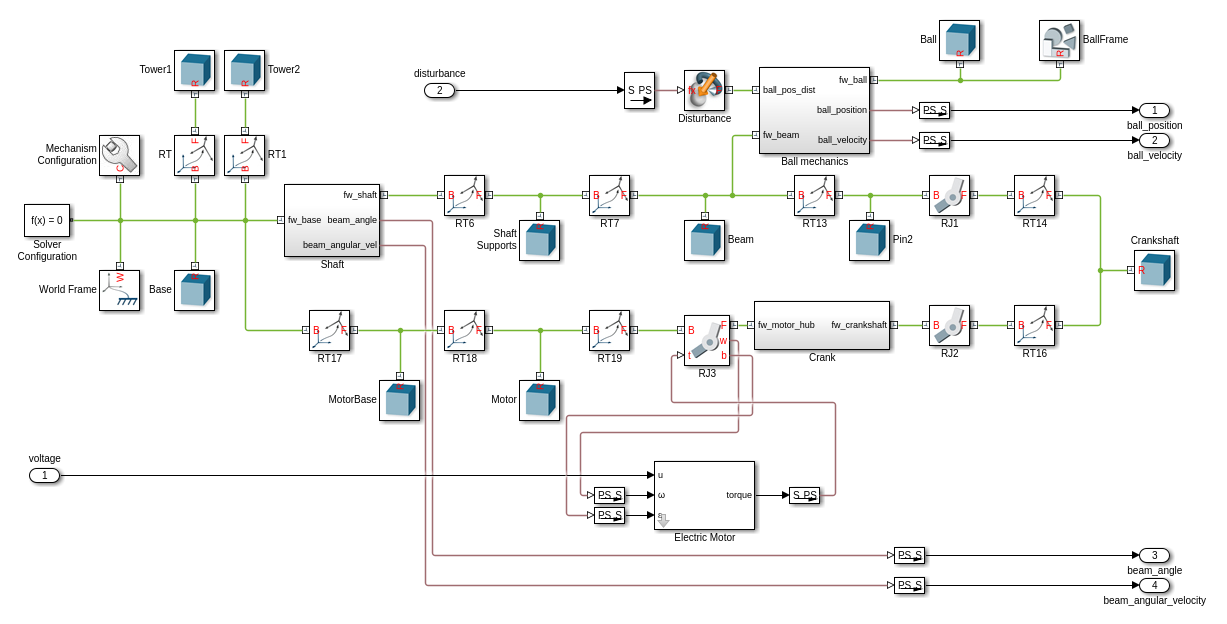
\includegraphics[width=\textwidth]{simmechanics_ballandbeam2}
    \caption{Schemat \textsc{SimMechanics} układu kulki i belki.}
    \label{fig:uklad_simmechanics2}
\end{sidewaysfigure}

Obiekty \textit{MotorBase} oraz \textit{Motor} reprezentują bryły podstawy, na której osadzony jest silnik oraz silnika. Elementy te nie biorą udziału w ogólnym zachowaniu belki pod wpływem momentu generowanego przez silnik, wobec czego nie nadano im skomplikowanych kształtów, jakie te elementy mają w~rzeczywistości.

\begin{figure}[h]
    \centering
    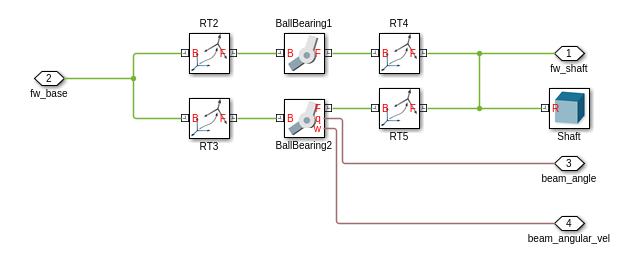
\includegraphics[width=0.8\textwidth]{simmechanics_shaft}
    \caption{Schemat podsystemu \textit{Shaft} odpowiadającego za umocowanie wału obrotu belki w danym układzie odniesienia.}
    \label{fig:sm_shaft}
\end{figure}

Sposób wykorzystania złącza obrotowego \textit{RJ3} został opisany w rozdziale \ref{sec:ch4_model_silnika}. Za wspomnianym złączem znajduje się podsystem \textit{Crank} (przedstawiony na \cref{fig:sm_shaft}), który składa się głównie z dwóch czarnych pinów (elementów mocujących o zerowej masie --- masa fizycznych przegubów włączona jest do masy korby bądź korbowodu) i korby (\textit{Crank}).

\begin{figure}[h]
    \centering
    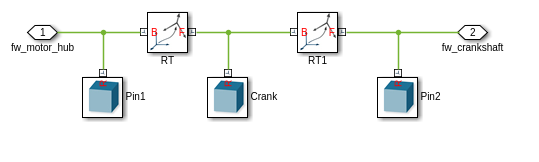
\includegraphics[width=0.8\textwidth]{simmechanics_crank}
    \caption{Schemat podsystemu \textit{Crank} odpowiadającego za umocowanie korby na wale motoreduktora.}
    \label{fig:sm_crank}
\end{figure}

Ostatnim, nieopisanym dotąd podsystemem, jest \textit{Ball mechanics} --- podsystem połączony z belką (\cref{fig:sm_ball_mechanics}), którego zadaniem jest ,,przytwierdzenie'' kulki do belki; osiągnięto to za pomocą nieopisanego dotąd bloku \textit{Rack and pinion} (pol. \textit{listwa (zębatka) współpracująca z kołem zębatym}).

Blok \textit{Rack and pinion} wymaga dla poprawnej pracy uzupełniania o dodatkowe elementy, na przykład w postaci złącz pryzmatycznego i obrotowego. Reprezentuje on więzy dla ruchu obrotowo-postępowego, z zerowym tarciem i~z~brakiem oderwania pod wpływem przyspieszeń pionowych, co dobrze przybliża zachowanie kulki w~układzie kulki i belki.

Połączenie równoległe bloków \textit{RPC1} i \textit{PJ}, \textit{RJ} przedstawione na \cref{fig:sm_ball_mechanics} spowodowane jest wymaganiami bloku \textit{Rack and pinion} co do osi przesuwu i osi obrotu; z tego powodu konieczne było użycie odpowiednich transformacji układów odniesienia \textit{RT12} oraz \textit{RT11}.

\begin{figure}[h]
    \centering
    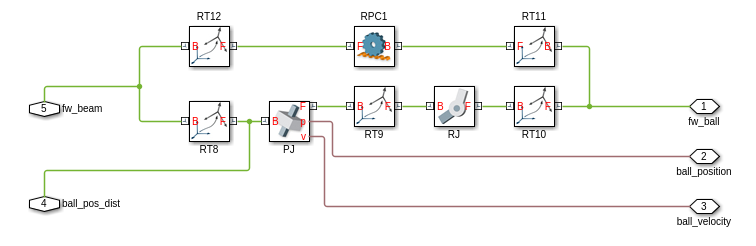
\includegraphics[width=0.9\textwidth]{simmechanics_ball_mechanics}
    \caption{Schemat podsystemu \textit{Ball mechanics} odpowiadającego za zachowanie kulki na belce.}
    \label{fig:sm_ball_mechanics}
\end{figure}

W układzie na \cref{fig:uklad_simmechanics2} jedno z wejść, oznaczone jako \textit{disturbance}, przeznaczone jest na symulowanie zewnętrznych zakłóceń wpływających bezpośrednio na kulkę; widoczne jest to w schemacie \textit{Ball mechanics} jako wejście \textit{ball\_pos\_dist}.

Z podsystemu \textit{Ball mechanics} wychodzą również dwa wyjścia: \textit{ball\_position} oraz \textit{ball\_velocity}. Odczytywane są one ze złącza pryzmatycznego kulki \textit{PJ}.

Sama kulka została dołączona do schematu poza podsystemem \textit{Ball mechanics}, jako ciało stałe \textit{Ball}. Równolegle dołączony blok \textit{BallFrame} odpowiada za wyświetlenie wersorów układu odniesienia środka kulki, co pomaga zobaczyć na wizualizacji faktyczny ruch obrotowy kulki po belce.

\section{Model silnika}
\label{sec:ch4_model_silnika}

Widoczny na \cref{fig:sm_electric_motor} model silnika prądu stałego odpowiada modelowi matematycznemu opartemu o równanie elektryczne obwodu silnika \eqref{eq:silnik_r_el} i równanie mechaniczne dla mas wirujących \eqref{eq:silnik_r_mech} (\cite{SILNIKIEL}):

\begin{equation}\label{eq:silnik_r_el}
    u - R i - L \deriv{i}{t} = K \omega 
\end{equation}
\begin{equation}\label{eq:silnik_r_mech}
    T = K i - J \epsilon - \beta \omega - b \sgn \omega
\end{equation}
gdzie:
\begin{itemize}
    \item $u$ --- napięcie sterujące,
    \item $R$ --- rezystancja silnika,
    \item $i$ --- prąd w obwodzie twornika,
    \item $K$ --- stała elektryczna bądź mechaniczna silnika (w jednostkach \si{\volt\second\per\radian} lub \si{\newton\meter\per\ampere}),
    \item $L$ --- indukcyjność silnika (w modelu na \cref{fig:sm_electric_motor} przyjęta za zerową),
    \item $T$ --- moment generowany przez silnik,
    \item $J$ --- moment bezwładności sprowadzony na wał motoreduktora,
    \item $\omega$ --- prędkość kątowa wału motoreduktora,
    \item $\epsilon = \deriv{\omega}{t}$ --- przyspieszenie kątowe wału motoreduktora,
    \item $\beta$ --- współczynnik tarcia wiskotycznego przekładni oraz silnika,
    \item $b$ --- współczynnik tarcia suchego przekładni oraz silnika.
\end{itemize}

\begin{figure}[h]
    \centering
    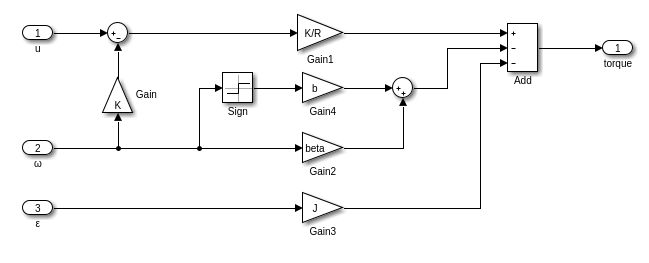
\includegraphics[width=0.8\textwidth]{simmechanics_electric_motor}
    \caption{Schemat podsystemu \textit{Electric Motor} odpowiadającego za model silnika prądu stałego.}
    \label{fig:sm_electric_motor}
\end{figure}

Warto zauważyć, że obliczanie kąta obrotu, prędkości kątowej oraz przyspieszenia kątowego odbywa się poza blokiem \textit{Electric Motor} --- wykonuje to \textsc{SimScape}, biorąc pod uwagę dynamikę reszty układu oraz moment, którym silnik działa na cały mechanizm.

W modelu silnika pominięto indukcyjność, gdyż jej wartość w rzeczywistości jest bardzo niska. Dodatkowo, przeprowadzona identyfikacja tarcia (rozdział \ref{sec:ch5_identyfikacja_parametrow_silnika}) pokazała, że poza tarciem mokrym w~układzie występuje pewne tarcie suche. Z powodu pracy silnika w sposób powtarzalny, tarcie suche może mieć spory wpływ na odpowiedź silnika, dlatego zdecydowano się go nie pomijać.

\section{Aproksymacja zależności kąta obrotu wału motoreduktora i osi belki}
\label{sec:ch4_zaleznosc_kata_silnika_i_kata_belki}

W związku z brakiem czujnika kąta obrotu wału belki, do odczytania jej położenia należy się posłużyć zależnością geometryczną od kąta obrotu wału motoreduktora. W rozdziale \ref{sec:ch3_uklad_napedowy} zasygnalizowano, że w pewnych niewielkich odchyleniach zależność ta może być opisana wzorem $\theta = \frac{L}{d_k} \alpha$.

Model symulacyjny \textsc{SimMechanics} eliminuje to ograniczenie, gdyż pozycja i prędkość wału belki odczytywane są bezpośrednio ze złącza obrotowego, w którym osadzony jest wspomniany wał. Niemniej jednak problem nadal występuje w rzeczywistym układzie, ponieważ nie zastosowano tam żadnego czujnika pozycji kątowej belki. Stąd postanowiono zmierzyć zależność $\theta(\alpha)$ poprzez symulację zbudowanego modelu. W tym celu podano stałe sterowanie na silnik i zmierzono jednocześnie kąt obrotu wału motoreduktora i wału belki.

\begin{figure}[h]
    \centering
    \includesvg[width=0.9\textwidth,svgpath=./vector_graphics/]{zaleznosc_kata2}
    \caption{Zależność kąta obrotu wału belki od kąta obrotu wału motoreduktora.}
    \label{fig:zaleznosc_kata_belki_od_enkodera}
\end{figure}

Należy zauważyć, że brak dobranych poprawnie parametrów silnika lub kulki nie wpływa negatywnie na dokładność aproksymacji, gdyż elementy łączące belkę z silnikiem są sztywne, a pomiar nie dotyczył dynamiki (prędkość, przyspieszenie) lecz statyki (obrót).

Obrót belki w funkcji obrotu wału motoreduktora postanowiono aproksymować sinusoidą (\cref{fig:zaleznosc_kata_belki_od_enkodera}) o następującym wzorze:
\begin{equation}\label{eq:aproksymacja_kata_walu}
    \theta(\alpha) = A \sin (\omega \alpha + \phi) + B
\end{equation}
gdzie:
\begin{itemize}
    \item $A$ --- amplituda sinusoidy,
    \item $\omega$ --- pulsacja,
    \item $\phi$ --- przesunięcie fazowe,
    \item $B$ --- wyraz wolny.
\end{itemize}

%Dane otrzymane po przeprowadzeniu aproksymacji numerycznej za pomocą funkcji \texttt{fminsearch} z programu \textsc{Matlab} pokazały, że kąt obrotu belki nie jest funkcją 
%Po przeprowadzeniu aproksymacji numerycznej za pomocą funkcji \texttt{fminsearch} z programu \textsc{Matlab} otrzymano 
Po przeprowadzeniu aproksymacji numerycznej za pomocą funkcji \texttt{fminsearch} z programu \textsc{Mat\-lab} otrzymano następujące wartości parametrów funkcji \eqref{eq:aproksymacja_kata_walu}: $A = \num{0.2387}$, $\omega = \num{1.0014}$, $\phi = \num{-1.5484}$, $B = \num{-0.05655}$; przybliżenie zostało przedstawione na \cref{fig:zaleznosc_kata_belki_od_enkodera}. Taka funkcja nie jest trudna do implementacji na sterowniku PLC, nie powinna również stanowić zbyt dużego wyzwania obliczeniowego\footnote{Producent deklaruje min. \SI{18}{\micro\second} dla obliczeń zmiennoprzecinkowych.} dla wybranego procesora (zob. tabelę \ref{tab:parametry_PLC_SB}).

Należy zauważyć, że wykres rzeczywistego kąta obrotu belki na \cref{fig:zaleznosc_kata_belki_od_enkodera} ma taki sam okres, jak wykres przybliżenia sinusoidą, a jednak kształt nie odpowiada mu całkowicie. Nie jest to błędem, gdyż w związku z działaniem w punkcie równowagi (zob. rozdział \ref{cha:ch6_model_liniowy}) największa dokładność przybliżenia oczekiwana jest w otoczeniu \SI[quotient-mode = fraction]{\pi/2}{\radian} kąta obrotu wału, czyli tam, gdzie oba wykresy są zbliżone.

\section{Podsumowanie}

W niniejszym rozdziale opisano sposób budowy modeli za pomocą przybornika narzędziowego \textsc{Simscape Multibody}, następnie przedstawiono i omówiono zbudowany w ten sposób model symulacyjny obiektu regulacji. W kolejnej części opisano model matematyczny silnika prądu stałego i jego implementację. Na końcu zaprezentowano wykorzystanie modelu obiektu do znalezienia zależności geometrycznej między kątem obrotu wału motoreduktora i wału belki.

%---------------------------------------------------------------------------
\chapter{Identyfikacja}
\label{cha:ch5_identyfikacja}

Używany w projekcie silnik prądu stałego nie posiada w dokumentacji wszystkich parametrów, jakie konieczne są, aby go zamodelować prawidłowo, a te parametry, które zostały podane, mają niepoprawne wartości. Wymusiło to ponowną identyfikację silnika --- częściowo eksperymentalną, częściowo numeryczno--optymalizacyjną.

Podobnie charakterystyki czujników odległości, chociaż podane przez producenta, wcale nie muszą odpowiadać wartościom rzeczywistym. Z racji wykorzystania w nich układów elektronicznych możliwa jest pewna wariancja w odpowiedziach --- nawet dla tych samych pobudzeń.

W niniejszym rozdziale przeprowadzono identyfikację nieznanych parametrów, a także weryfikację tych podanych przez producenta.

%%%%
\section{Identyfikacja charakterystyk czujników odległości}
\label{sec:ch5_identyfikacja_charakterystyk_czujnikow}

W celu pobrania charakterystyk indywidualnych czujników przeprowadzono serię eksperymentów, w których zmierzono odpowiedzi czujników w zależności od pozycji przeszkody. Użytą przeszkodą była kulka (zob. rozdział \ref{sec:ch2_kulka}).

Procedura pojedynczego eksperymentu przeprowadzana była następująco: kulkę zamieszczano tak, aby jej środek znajdował się na wybranej pozycji; następnie kulka była zabezpieczana taśmą, aby jej położenie nie uległo zmianie w trakcie eksperymentu. Próbki pobierane były z dwóch przetworników ADC co \SI{100}{\milli\second} przez kilkadziesiąt sekund (przynajmniej pół minuty). W efekcie dla każdego wyznaczonego położenia kulki do dalszej analizy dostępnych było kilkaset próbek.

Pobieranie próbek odbywało się poprzez narzędzie \texttt{Traces} z programu \textsc{Siemens TIA Portal}, które umożliwia eksport wyników do formatu \texttt{.csv} w celu dalszej obróbki.

Z każdej serii próbek odpowiadającej jednej pozycji środka kulki wyliczono średnią arytmetyczną wartości z~obu przetworników. Przyjęto, że wartości te odpowiadają odpowiedziom czujników na odległość do bliższej im krawędzi kulki; to założenie jest słuszne dlatego, że do pomiaru środka kulki wykorzystana jest para czujników i~wartość średnia ich odczytów (por. rozdział \ref{sec:ch3_czujniki_odleglosci}, szczególnie wzór~\eqref{eq:pozycja_kulki}).

Wykres uzyskanych danych pomiarowych został przedstawiony na \cref{fig:charakterystyka_czujnikow}, natomiast dane przygotowane do przeprowadzenia aproksymacji umieszczone są w tabeli \ref{tab:pomiary_czujniki}. Dane te zostały skrócone, tzn. wyeliminowano pomiar dla odległości mniejszych od \SI{3}{\centi\meter}, który wprowadzał dwuznaczność do odwzorowania \textit{pomiar$\,\to\,$odległość}.

\begin{table}[H]
    \centering
    \caption{Uzyskane wyniki pomiarów charakterystyk każdego z czujników.}
    \label{tab:pomiary_czujniki}

    \begin{tabularx}{0.9\textwidth}{c | S | S}
        \toprule
        Odległość do piłki & {Wartość z ADC czujnika lewego} & {Wartość z ADC czujnika prawego} \\
        \midrule
        % \SI{2}{\centi\meter} & 7780,799615 & 7387,194313 \\ % wprowadza dwuznaczność
        \SI{3}{\centi\meter} & 8318,137584 & 8364,10453 \\
        \SI{4}{\centi\meter} & 7340,2222 & 6993,866279 \\
        \SI{5}{\centi\meter} & 6053,363328 & 5767,105651 \\
        \SI{6}{\centi\meter} & 5216,61082 & 5029,89899 \\
        \SI{7}{\centi\meter} & 4366,262745 & 4334,347917 \\
        \SI{8}{\centi\meter} & 3956,949782 & 3875,203271 \\
        \SI{9}{\centi\meter} & 3629,119926 & 3501,318182 \\
        \SI{10}{\centi\meter} & 3264,490872 & 3120,025641 \\
        \SI{11}{\centi\meter} & 2902,293996 & 2815,218324 \\
        \SI{12}{\centi\meter} & 2685,820809 & 2594,338488 \\
        \SI{13}{\centi\meter} & 2560,291417 & 2426,931271 \\
        \SI{14}{\centi\meter} & 2354,944805 & 2217,032895 \\
        \SI{15}{\centi\meter} & 2191,632399 & 2091,435986 \\
        \SI{16}{\centi\meter} & 2066,078067 & 1970,516373 \\
        \SI{17}{\centi\meter} & 1944,336323 & 1806,977578 \\
        \SI{18}{\centi\meter} & 1756,851385 & 1699,710037 \\
        \SI{19}{\centi\meter} & 1677,359862 & 1611,165109 \\
        \SI{20}{\centi\meter} & 1603,756579 & 1527,873377 \\
        \SI{21}{\centi\meter} & 1492,209622 & 1380,49501 \\
        \SI{22}{\centi\meter} & 1435,164948 & 1346,626204 \\
        \SI{23}{\centi\meter} & 1368,446394 & 1271,832298 \\
        \SI{24}{\centi\meter} & 1313,357143 & 1199,407708 \\
        \SI{25}{\centi\meter} & 1251,582888 & 1153,330258 \\
        \SI{26}{\centi\meter} & 1206,343458 & 1109,593886 \\
        \SI{27}{\centi\meter} & 1157,610417 & 1077,421569 \\
        \SI{28}{\centi\meter} & 1113,545455 & 1024,010471 \\
        \SI{29}{\centi\meter} & 1074,938575 & 991,7826825 \\
        \SI{30}{\centi\meter} & 1028,267442 & 955,1822222 \\
        \SI{31}{\centi\meter} & 979,5052265 & 930,057047 \\
        \SI{32}{\centi\meter} & 960,6421801 & 904,1445087 \\
        \bottomrule
    \end{tabularx}
\end{table}

Aproksymacja charakterystyk czujników została przeprowadzona za pomocą narzędzia \texttt{Curve Fitting} z programu \textsc{Matlab}. Najlepsze przybliżenia otrzymano przy wykorzystaniu aproksymacji wykładniczej (zob. \cref{fig:aproksymacja_czujnika_lewego}, \cref{fig:aproksymacja_czujnika_prawego}), tj. postaci $y = a x^b + c$, gdzie $x$ to wartość pomiaru z przetwornika, a $y$ to odległość do przeszkody. Odpowiednie funkcje przedstawiono w tabeli \ref{tab:aproksymacja_czujnikow}.

\begin{table}[h]
    \centering
    \caption{Funkcje aproksymujące charakterystyki czujników.}
    \label{tab:aproksymacja_czujnikow}
    
    \begin{tabularx}{0.62\textwidth}{l | l | S}
        \toprule
        Czujnik & Funkcja aproksymująca & {Wartość błędu \textit{RSME}} \\
        \midrule
        Lewy  & $y = 9819 x ^ {-0,8229} - \num{2,651} $ & 0,197 \\
        Prawy & $y = 8166 x ^ {-0,8055} - \num{2,525} $ & 0,2639 \\
        \bottomrule
    \end{tabularx}
\end{table}

\begin{figure}[h]
    \centering
    \includesvg[width=1\textwidth,svgpath=./vector_graphics/]{aproksymacja_czujnika_lewego}
    \caption{Wykres przedstawiający aproksymację charakterystyki czujnika lewego.}
    \label{fig:aproksymacja_czujnika_lewego}
\end{figure}

\begin{figure}[H]
    \centering
    \includesvg[width=1\textwidth,svgpath=./vector_graphics/]{aproksymacja_czujnika_prawego}
    \caption{Wykres przedstawiający aproksymację charakterystyki czujnika prawego.}
    \label{fig:aproksymacja_czujnika_prawego}
\end{figure}

W ramach eksperymentów przeprowadzono również test zachowania czujników, gdy pomiędzy nimi nie ma żadnej przeszkody. Pozwoliło to oszacować wartości progowe, które użyte zostały do oszacowania braku lub obecności kulki. Więcej szczegółów umieszczono w~rozdziale \ref{sec:ch7_wykrywanie_braku_kulki}.

\section{Identyfikacja parametrów silnika}
\label{sec:ch5_identyfikacja_parametrow_silnika}

Jak to zostało zasygnalizowane we wstępie do rozdziału, nie wszystkie parametry silnika są poprawne lub zostały podane przez producenta. Spośród podanych przez producenta (zob. tab. \ref{tab:parametry_silnika}) do zweryfikowania możliwe są:

\begin{itemize}
    \item napięcie zasilania silnika $u_N$,
    \item prędkość biegu jałowego odpowiadającego temu napięciu $\omega_N$,
    \item prąd biegu jałowego $i_N$.
\end{itemize}

Niestety niemożliwe jest zweryfikowanie prądu zatrzymania silnika $i_S$, tj. prądu pobieranego przez silnik przy napięciu znamionowym oraz fizycznym zablokowaniu obrotu wału silnika. Doprowadzenie do takiej sytuacji spowodowałoby fizyczne uszkodzenie zasilacza, mostka H lub samego silnika. Z~identycznych powodów niemożliwe jest zmierzenie momentu koniecznego do zatrzymania obrotu wału motoreduktora w tych samych warunkach.

\subsection{Weryfikacja parametrów podanych przez producenta silnika}
\label{subsec:ch5_weryfikacja_parametrow_producenta_silnika}

Poniższe pomiary i eksperymenty wykonano przy nieobciążonym silniku, tj. po rozłączeniu połączenia wału motoreduktora z korbą.

Za pomocą multimetru zmierzono napięcie na stykach zasilacza przeznaczonego dla silnika (zob. rozdział \ref{sec:ch3_systemy_napiec}), które wyniosło \SI{11,95}{\volt}. Również za pomocą multimetru, tym razem wpinając się szeregowo w obwód zasilania silnika, zmierzono prąd biegu jałowego, którego natężenie wyniosło \SI{0,23}{\ampere}.

Prędkość biegu jałowego silnika wyznaczono za pomocą eksperymentu: na silnik podano maksymalne sterowanie, a za pomocą narzędzia \texttt{Traces} z programu \textsc{Siemens TIA Portal} pobrano odpowiedź silnika (wartość licznika enkodera); próbkowanie w tym eksperymencie wyniosło około \SI{1}{\milli\second}. Następnie dla części danych, dla których silnik osiągnął stałą wartość prędkości, wyznaczono nachylenie. Wartość tego nachylenia odpowiada prędkości kątowej wału motoreduktora, co zaprezentowano na \cref{fig:odpowiedz_silnika_na_maksymalny_skok_jednostkowy}.

Z powyższego eksperymentu uzyskano wartość prędkość kątowej biegu jałowego \SI{58,267}{\radian\per\second}.

\begin{figure}[h]
    \centering
    \includesvg[width=0.7\textwidth,svgpath=./vector_graphics/]{predkosc_biegu_jalowego}
    \caption{Wykres odpowiedzi silnika na skok jednostkowy (maksymalne napięcie) z~zaznaczoną prostą, której nachylenie odpowiada prędkości kątowej wału motoreduktora.}
    \label{fig:odpowiedz_silnika_na_maksymalny_skok_jednostkowy}
\end{figure}

\subsection{Identyfikacja parametrów niepodanych przez producenta silnika}
\label{subsec:ch5_identyfikacja_parametrow_niepodanych_przez_producenta_silnika}

Pozostałe parametry, wymagane do poprawnego działania modelu silnika (zob. rozdział \ref{sec:ch4_model_silnika}), których wartości nie zostały podane przez producenta, to:

\begin{itemize}
    \item rezystancja silnika $R$,
    \item stała silnika $K$,
    \item indukcyjność silnika $L$,
    \item współczynniki tarcia wiskotycznego $\beta$ oraz suchego $b$,
    \item moment bezwładności wału motoreduktora $J$.
\end{itemize}

Wartości tych parametrów zostały najpierw obliczone analitycznie, a następnie zoptymalizowane numerycznie.

Rezystancję $R$ obliczono z równania elektrycznego silnika \eqref{eq:silnik_r_el} dla sytuacji zatrzymania silnika ($\omega = 0$, $i = i_S$). Mamy wtedy:

\begin{equation}
    R = \frac{u_N}{i_S} = \frac{\num{11,95}}{\num{5}} = \SI{2,39}{\ohm}
\end{equation}

Z tego samego równania \eqref{eq:silnik_r_el} dla pracy jałowej silnika można wyciągnąć zależność na stałą silnika~$K$:

\begin{equation}
    K = \frac{u_N - R i_N}{\omega_N} = \frac{\num{11,95} - \num{2,39} \cdot \num{0,23}}{\num{58,267}} = \num{0,195656203}
\end{equation}

Jednostką stałej $K$ jest \si{\newton\meter\per\ampere} (dla stałej momentu) lub \si{\volt\second\per\radian} (dla stałej SEM rotacji).

Zależności na współczynniki tarcia wiskotycznego i suchego można natomiast wyciągnąć z równania mechanicznego silnika \eqref{eq:silnik_r_mech} działającego przy ustalonej prędkości kątowej ($\dot{\omega} = 0$):

\begin{align}
    K i &= \beta \omega + b \sgn \omega \nonumber \\
    \frac{K}{R} (u - K \omega) &= \beta \omega + b \sgn \omega \nonumber \\
    \frac{K}{R} u &= \left(\frac{K^2}{R} + \beta \right) \omega + b \sgn \omega \nonumber \\
    \omega &= \frac{K}{R \left(\frac{K^2}{R} + \beta \right)} u + \frac{b}{\frac{K^2}{R} + \beta} \sgn \omega \label{eq:predkosc_obrotowa_walu}
\end{align}

Możliwe jest wyznaczenie analityczne zależności dla $\beta$ \eqref{eq:zaleznosc_beta} oraz $b$ \eqref{eq:zaleznosc_b} na podstawie wzoru \eqref{eq:predkosc_obrotowa_walu}, jeśli przyjąć, że jest to wzór określający liniową zależność postaci $\omega(u) = K_1 u + K_2$:

\begin{align}
    K_1 &= \frac{K}{R \left(\frac{K^2}{R} + \beta \right)} \nonumber \\
    R K_1 \left(\frac{K^2}{R} + \beta \right) &= K \nonumber \\
    \beta &= \frac{K - K_1 K^2}{R K_1} \label{eq:zaleznosc_beta}
\end{align}

\begin{align}
    K_2 &= \frac{b}{\frac{K^2}{R} + \beta} \nonumber \\
    b &= K_2 \left(\frac{K^2}{R} + \beta \right) \label{eq:zaleznosc_b}
\end{align}

W wyprowadzeniu \eqref{eq:zaleznosc_b} pominięto kwestie zgodności znaku (nieciągłość wprowadzona przez~$\sgn \omega$).
% ; należy jednak spodziewać się dodatnich wartości obu współczynników jako wielkości fizycznych.
%  Mnożenie przez $\sgn \omega$ ma na celu jedynie wskazanie, że siła tarcia suchego przeciwdziała ruchowi 

Współczynniki $K_1$ oraz $K_2$ uzyskano przeprowadzając eksperymenty odpowiedzi skokowych silnika dla kilkudziesięciu kolejnych wartości sterowań, pokrywających cały dopuszczalny zakres. Na podstawie danych pomiarowych, na które składają się sterowanie i~wartość licznika enkodera, obliczono prędkość ustaloną silnika dla każdego sterowania, co przedstawia tabela \ref{tab:predkosc_silnika_rozne_sterowania}.

Wykres danych z tabeli \ref{tab:predkosc_silnika_rozne_sterowania}, wraz z naniesionymi przybliżeniami (krzywymi regresji liniowych) uzyskanymi z narzędzia \texttt{Curve Fitting} z programu \textsc{Matlab}, został przedstawiony na \cref{fig:predkosci_obrotowe_silnika}. Jak widać, krzywe regresji nie przecinają się w punkcie $(0, 0)$, co oznacza, że wyraz wolny równania \eqref{eq:predkosc_obrotowa_walu} jest niezerowy, a zatem współczynnik $b$ również jest niezerowy. Dowodzi to, że słusznie wzięto pod uwagę w modelu silnika tarcie suche.

%\pagebreak

\begin{table}[H]
    \centering
    \begin{threeparttable}
        \caption{Prędkość kątowa silnika dla różnych sterowań.}
        \label{tab:predkosc_silnika_rozne_sterowania}
        
        \begin{tabularx}{0.7\textwidth}{r | S[round-mode=places, round-precision=3] | S[round-mode=places, round-precision=2]}
            \toprule
            {Sterowanie\tnote{a}} & {Napięcie\tnote{b} \si{[\volt]}} & {Prędkość kątowa \si{[\radian\per\second]}} \\
            \midrule
            \SI{-100}{\percent} & -11,95 & -59,1747823797\tnote{c} \\
            \SI{-90}{\percent} & -10,755 & -53,5556835151 \\
            \SI{-80}{\percent} & -9,56 & -47,7764908354 \\
            \SI{-70}{\percent} & -8,365 & -41,4676492 \\
            \SI{-60}{\percent} & -7,17 & -35,4980443085 \\
            \SI{-50}{\percent} & -5,975 & -29,321762139 \\
            \SI{-40}{\percent} & -4,78 & -23,4432023973 \\
            \SI{-30}{\percent} & -3,585 & -17,3397328183 \\
            \SI{-20}{\percent} & -2,39 & -11,2885697 \\
            \SI{-15}{\percent} & -1,7925 & -7,6263495 \\
            \SI{-10}{\percent} & -1,195 & -5,2389469 \\
            \SI{-5}{\percent} & -0,5975 & -1,4984893 \\
            % 0 & 0 & 0 \\
            \SI{5}{\percent} & 0,5975 & 1,5175142842 \\
            \SI{10}{\percent} & 1,195 & 5,2958385151 \\
            \SI{15}{\percent} & 1,7925 & 7,6516988362 \\
            \SI{20}{\percent} & 2,39 & 11,2804252886 \\
            \SI{30}{\percent} & 3,585 & 17,3147742373 \\
            \SI{40}{\percent} & 4,78 & 23,3701426292 \\
            \SI{50}{\percent} & 5,975 & 29,4408026601 \\
            \SI{60}{\percent} & 7,17 & 35,4943644178 \\
            \SI{70}{\percent} & 8,365 & 41,5480352978 \\
            \SI{80}{\percent} & 9,56 & 47,7366740427 \\
            \SI{90}{\percent} & 10,755 & 53,8652645807 \\
            \SI{100}{\percent} & 11,95 & 59,1984746765 \\
            \bottomrule
        \end{tabularx}
        
        \begin{tablenotes}
            \footnotesize
            \item[a] wypełnienie sygnału PWM, przy czym znak sterowania zmienia drugi sygnał kierunku obrotów (zob. rozdział \ref{sec:ch3_uklad_napedowy}),
            \item[b] efektywne napięcie (wprost proporcjonalne do napięcia sygnału PWM),
            \item[c] wartość różna o około \SI{1}{\radian\per\second} od zmierzonej prędkości ustalonej podanej w rozdziale \ref{subsec:ch5_weryfikacja_parametrow_producenta_silnika}; pewne implikacje tej różnicy opisano w rozdziale \ref{sec:ch5_weryfikacja_identyfikacji_silnika}.
        \end{tablenotes}
    \end{threeparttable}
\end{table}

Współczynniki regresji liniowych $K_1$, $K_2$ wraz z obliczonymi na ich podstawie wartościami współczynników tarcia $\beta$ oraz $b$ zostały przedstawione w tabeli \ref{tab:param_regresji_lin_wsp_tarcia}. W dalszych rozważaniach przyjęto wartość uśrednioną z obu wyników: $\beta = \num{8,2436e-5}$, $b = \num{0,017283013}$.

\begin{figure}[p]
    \centering
    \includesvg[width=1\textwidth,svgpath=./vector_graphics/]{tarcie}
    \caption{Wykres ustalonych prędkości kątowych silnika w zależności od podanego sterowania.}
    \label{fig:predkosci_obrotowe_silnika}
\end{figure}

\begin{table}[p]
    \centering
    \begin{threeparttable}
        \caption{Parametry regresji liniowych i współczynniki tarcia.}
        \label{tab:param_regresji_lin_wsp_tarcia}
        
        \begin{tabular}{l | S[round-mode=places, round-precision=6] | S[round-mode=places, round-precision=6]}
            \toprule
            Współczynnik & {Wartość dla prędkości ujemnej} & {Wartość dla prędkości dodatniej} \\
            \midrule
            $K_1$ & 5.080320730295036 & 5.089359196349887 \\
            $K_2$ & 1.068028629228871 & -1.078974349431031 \\
            $\beta$ & 9.674447407874083e-05 & 6.812667587453827e-05 \\
            $b$\tnote{a} & 0.017210262069886 & 0.017355764034522 \\
            \bottomrule
        \end{tabular}
        
        \begin{tablenotes}
            \footnotesize
            \item[a] Postawiono znak dodatni tak, aby wzór \eqref{eq:predkosc_obrotowa_walu}, uwzględniający nieciągłość $\sgn \omega$, był poprawny.
        \end{tablenotes}
    \end{threeparttable}
\end{table}

\pagebreak

Zidentyfikowano zatem następujące parametry silnika:
\begin{itemize}
    \item rezystancja silnika $R$,
    \item stała silnika $K$,
    \item współczynniki tarcia wiskotycznego $\beta$ oraz suchego $b$.
\end{itemize}

Należy zauważyć, że wszystkie te parametry zależą bezpośrednio ($R$) lub pośrednio ($K$, $\beta$, $b$) od wartości prądu zatrzymania silnika $i_S$, której nie można zmierzyć bez niszczenia elementów obiektu, a~należy podejrzewać, że wartość przedstawiona przez producenta nie jest prawidłowa. W związku z~tym istnieją podstawy, by przeprowadzić dodatkową optymalizację wyznaczonych wartości wspomnianych parametrów. Razem z nią zidentyfikować można pozostałe, brakujące parametry --- indukcyjność obwodów silnika $L$ oraz moment bezwładności wału $J$.

\subsection{Identyfikacja parametrów metodami optymalizacji numerycznej}
\label{subsec:ch5_identyfikacja_parametrow_metodami_optymalizacji_numerycznej}

Do identyfikacji wykorzystano model zbliżony do modelu z \cref{fig:sm_electric_motor}, również oparty o równania elektryczne \eqref{eq:silnik_r_el} i mechaniczne silnika \eqref{eq:silnik_r_mech}. Został on przedstawiony na \cref{fig:electric_motor}. Główną różnicą w~stosunku do modelu ze schematu symulacyjnego obiektu jest brak polegania na mechanice przybornika narzędziowego \textsc{SimScape Multibody} w celu wyliczenia momentu, prędkości obrotowej czy przyspieszenia kątowego.

\begin{figure}[h]
    \centering
    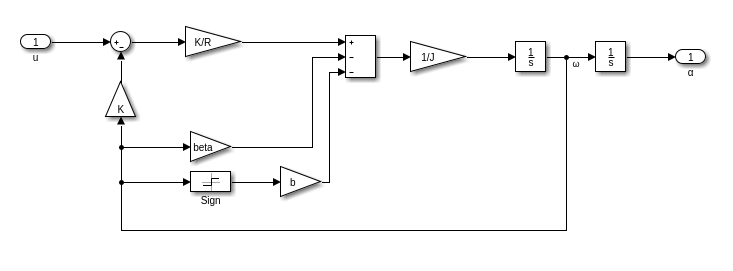
\includegraphics[width=1\textwidth]{electric_motor}
    \caption{Schemat modelu silnika prądu stałego użytego do identyfikacji parametrów.}
    \label{fig:electric_motor}
\end{figure}

Optymalizacja została przeprowadzona za pomocą narzędzia \texttt{Parameter Estimation} z pakietu \textsc{Matlab/Simulink}. Wykorzystuje ono z góry zadane sterowanie i znaną odpowiedź rzeczywistego obiektu do takiego dobrania parametrów, aby odpowiedź modelu była jak najbliższa rzeczywistej.

Jako zadane sterowanie wykorzystano zapisany za pomocą narzędzia \texttt{Traces} z programu \textsc{Siemens TIA Portal} kilkukrotny skok jednostkowy sterowania; podobnie użytą odpowiedzią obiektu była zapisana wartość licznika enkodera przeliczona na kąt obrotu belki. Za początkowe wartości parametrów przyjęto wartości obliczone w poprzednich rozdziałach, a w przypadku momentu bezwładności wału motoreduktora przyjęto $J = \SI{0,0014}{\kilogram\meter\squared}$.

Dane wejściowe, wyjściowe i odpowiedź modelu przedstawiono na \cref{fig:silnik_oszacowanie_parametrow}, a wyniki końcowe estymacji zostały umieszczone w tabeli \ref{tab:parametry_silnika_optymalizacja}.

\begin{table}[h]
    \centering
    \begin{threeparttable}
        \caption{Parametry silnika przed i po optymalizacji.}
        \label{tab:parametry_silnika_optymalizacja}
        
        \begin{tabular}{c | S[round-mode=places, round-precision=6] | S[round-mode=places, round-precision=6] | c}
            \toprule
            Parametr & {Wartość przed optymalizacją} & {Wartość po optymalizacji} & Względna zmiana wartości \\
            \midrule
            $b$ & 0.017283013 & 0.0141323209897433 & \SI{-18,23}{\percent} \\
            $\beta$ & 0.000082436 & 2.39578033890406e-05 & \SI{-70,34}{\percent} \\
            $J$ & 0.0014 & 0.000980836189992714 & \SI{-29,94}{\percent} \\
            $K$ & 0.195656203 & 0.206891906758788 & \SI{5,74}{\percent} \\
            $R$ & 2.39 & 2.54024084288707 & \SI{6,29}{\percent} \\
            \bottomrule
        \end{tabular}
    \end{threeparttable}
\end{table}
% TODO: skomentować zmianę bety?

\begin{figure}[H]
    \centering
    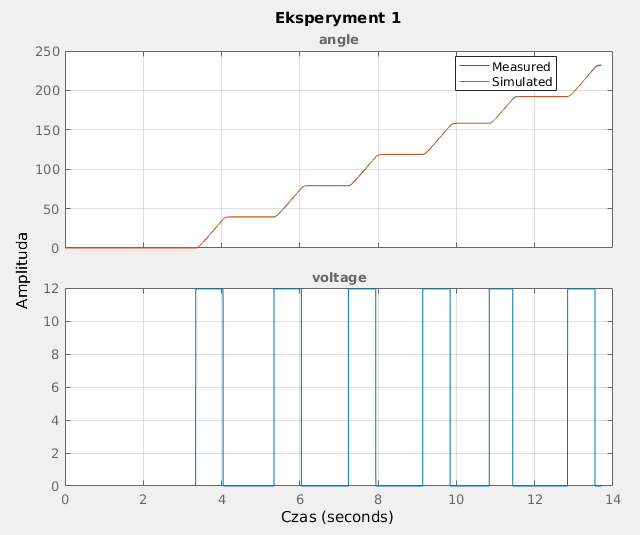
\includegraphics[width=0.8\textwidth]{optymalizacja_exp1}
    \caption{Zrzut ekranu wykresów danych wejściowych (dół) i wyjściowych dla procesu optymalizacji oraz odpowiedź obiektu po przeprowadzonej optymalizacji parametrów (góra).}
    \label{fig:silnik_oszacowanie_parametrow}
\end{figure}

Jak widać z \cref{fig:silnik_oszacowanie_parametrow}, dopasowanie odpowiedzi modelu do odpowiedzi obiektu rzeczywistego jest bardzo dobre, nawet bez uwzględnienia indukcyjności obwodów silnika. Oznacza to, że wartość parametru $L$ jest zaniedbywalna.

%%%%
\section{Weryfikacja identyfikacji silnika}
\label{sec:ch5_weryfikacja_identyfikacji_silnika}

Narzędzie \texttt{Parameter Estimation} z pakietu \textsc{Matlab/Simulink} poza optymalizacją parametrów modelu umożliwia również weryfikację działania modelu opartego o te parametry. Weryfikacja odbywa się przy użyciu innych danych niż optymalizacja.

Pierwszą weryfikację przeprowadzono z wykorzystaniem ,,ujemnych'' skoków jednostkowych, tj. sterowania silnika skierowanego w przeciwną stronę. Wyniki zostały zaprezentowane na \cref{fig:silnik_weryfikacja_parametrow}. Jak widać, dobrane numerycznie parametry modelu silnika dają w tym przypadku zadowalające rezultaty.

\begin{figure}[h]
    \centering
    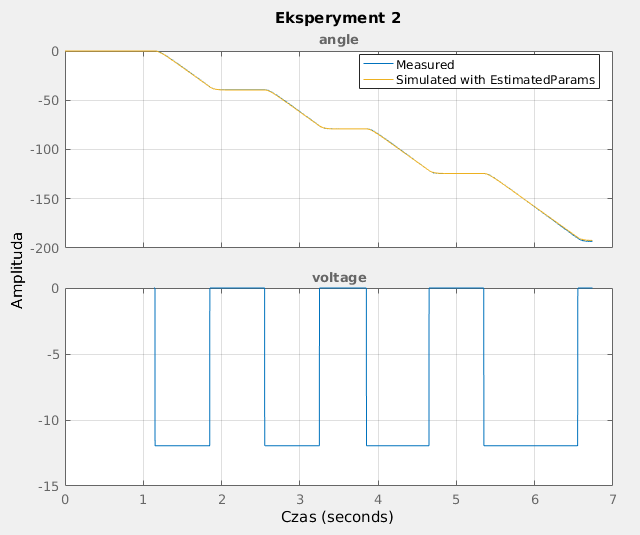
\includegraphics[width=0.7\textwidth]{walidacja_exp2}
    \caption{Zrzut ekranu wykresów danych wejściowych (dół) i wyjściowych dla procesu weryfikacji oraz odpowiedź obiektu ze zoptymalizowanymi parametrami (góra).}
    \label{fig:silnik_weryfikacja_parametrow}
\end{figure}

Druga weryfikacja, w której sterowaniem w danych wejściowych były pojedyncze skoki o wartościach \SIlist{100;-100;50;-50}{\percent}, nie przyniosła tak dobrych rezultatów (\cref{fig:silnik_nieudana_weryfikacja_parametrow}). Być może jest to wynikiem osiągania innych prędkości ustalonych przez silnik, co zostało zaznaczone wcześniej w rozdziałach \ref{subsec:ch5_weryfikacja_parametrow_producenta_silnika} oraz \ref{subsec:ch5_identyfikacja_parametrow_niepodanych_przez_producenta_silnika}. Niemniej jednak, różnica w osiągach silnika nie jest wielka, zatem należy się spodziewać, że zaprojektowane sprzężenie zwrotne pozwoli te różnice zminimalizować.

\begin{figure}[h]
    \centering
    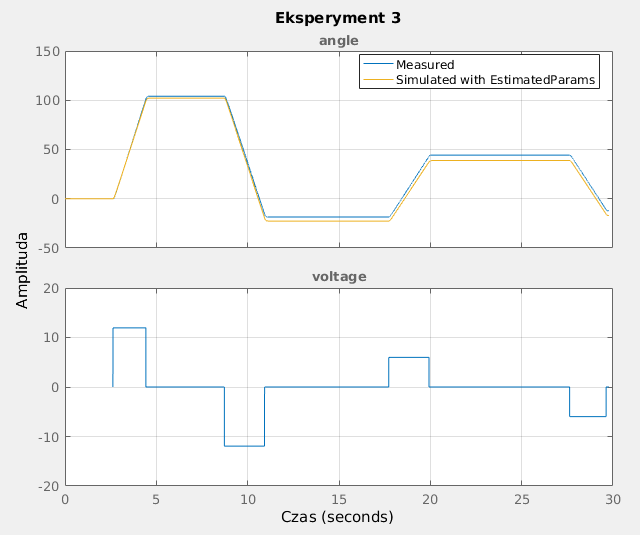
\includegraphics[width=0.7\textwidth]{walidacja_exp3}
    \caption{Zrzut ekranu wykresów danych wejściowych (dół) i wyjściowych dla procesu weryfikacji przy kolejnym eksperymencie.}
    \label{fig:silnik_nieudana_weryfikacja_parametrow}
\end{figure}

%%%%
% \section{Identyfikacja momentu bezwładności kulki}
% \label{sec:ch5_identyfikacja_bezwladnosci_kulki}

% TODO: skonsultować wyniki z drem Tutajem

%%%%
\section{Podsumowanie}

W niniejszym rozdziale przedstawiono sposób wyznaczenia charakterystyk czujników odległości oraz identyfikację parametrów silnika prądu stałego. Parametry silnika, które zostały podane przez producenta, okazały się niedokładne, dlatego w pierwszej kolejności zweryfikowano je --- o ile było to możliwe. Następnie na podstawie równań elektrycznego i mechanicznego silnika wyznaczono prawie wszystkie nieznane parametry. W ostatnim kroku zidentyfikowano numerycznie pozostałe parametry oraz zoptymalizowano już wyznaczone, co potwierdziła opisana weryfikacja wyników identyfikacji parametrów silnika.

%---------------------------------------------------------------------------
\chapter{Model liniowy obiektu i regulacja}
\label{cha:ch6_model_liniowy}

Do wyznaczenia regulatorów dla systemu konieczne jest uzyskanie jego uproszczonego modelu liniowego, który --- w myśl twierdzenia Hartmana-Grobmana --- zachowuje się podobnie jak obiekt nieliniowy. Zgodnie z teorią sterowania, wyznaczone w tym rozdziale regulatory powinny działać w odchyłkach wybranego punktu pracy.

%%%%
\section{Punkt pracy i linearyzacja}
\label{sec:ch6_punkt_pracy_linearyzacja}

Za zmienne stanu przyjęto: położenie liniowe kulki względem środka belki $x_1$, kąt obrotu belki względem poziomu $x_3$ oraz ich pochodne w czasie $x_2 = \dot{x_1}$, $x_4 = \dot{x_3}$.

\begin{figure}[h]
    \centering
    \includesvg[width=0.5\textwidth,svgpath=./vector_graphics/]{zmienne_stanu}
    \caption{Reprezentacja głównych zmiennych stanu w obiekcie.}
    \label{fig:zmienne_stanu}
\end{figure}

Jak naturalny wybrano punkt pracy $x^*$, w którym wszystkie zmienne stanu są zerowe:
\begin{equation}
    x^* = \begin{bmatrix}
    0 \\
    0 \\
    0 \\
    0 \\
    \end{bmatrix}
\end{equation}

Linearyzację modelu przeprowadzono z wykorzystaniem narzędzi wbudowanych w pakiet \textsc{Mat\-lab/Si\-mu\-link}, a konkretnie \texttt{Linear Analysis Tool}. Do linearyzacji przygotowano wersję mo\-de\-lu układu z odłączonym wejściem na zakłócenia oraz wyłączoną (za pomocą bloku \textit{Manual Switch}) częścią odpowiedzialną za symulację tarcia suchego w silniku (\cref{fig:sm_linearization}). Usunięcie tarcia suchego w~przypadku linearyzacji w punkcie równowagi $x^*$ spowodowane jest względami praktycznymi: częsta zmiana znaku prędkości obrotowej belki utrudnia lub nawet uniemożliwia uruchamianie symulacji, gdyż wewnętrzny mechanizm \textsc{Simulink} wykrywa wtedy wiele przejść przez zero\footnote{Możliwe jest wyłączenie tego mechanizmu lub użycie metody adaptacyjnej wykrywania przejść przez zero, jednakże spowalnia to symulację.}.

\begin{figure}[h]
    \centering
    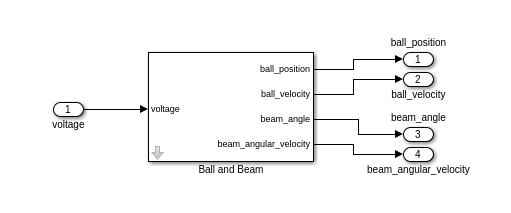
\includegraphics[width=0.9\textwidth]{sm_linearization}
    \caption{Model układu przeznaczony do przeprowadzenia linearyzacji.}
    \label{fig:sm_linearization}
\end{figure}

Przed linearyzacją konieczne było znalezienie punktu pracy, czyli przeprowadzenie tzw. \textit{trimmingu} modelu. W procesie tym wyznacza się ograniczenia na stany układu lub ich wartości początkowe. Jest to istotne zagadnienie, gdyż układ zbudowany za pomocą przybornika \textsc{Simscape Multibody} zawiera \num{18} stanów, chociaż, tak jak to zdefiniowano na początku rozdziału, wybrano jedynie \num{4} do prezentacji systemu. Większość z tych ,,nadmiarowych'' stanów to położenia i prędkości złącz pryzmatycznych lub obrotowych, które nie są istotne z punktu widzenia reprezentacji liniowej układu.

\textit{Trimming} modelu to tak naprawdę proces optymalizacyjny, mający na celu tak dobrać wartości początkowe stanów systemu, aby maksymalny ich błąd w trakcie symulacji był jak najmniejszy; jest to jednoznaczne z numerycznym znajdowaniem punktu równowagi systemu. Z powodu swojej optymalizacyjnej natury, proces ten nie mógł znaleźć odpowiedniego punktu, dopóki nie został rozpoczęty z odpowiednio bliskiego otoczenia punktu równowagi. Osiągnięto to podając jako wartość startową dla wejścia bloku (\textit{voltage} na \cref{fig:sm_linearization}) napięcie sterowania $u = -0,51158$. Wartość ta wynika z faktu delikatnego ciążenia belki w stronę mechanizmu korbowego, co musi rekompensować silnik poprzez wytworzenie niezerowego momentu.

Po wyznaczeniu punktu równowagi, nadal wykorzystując narzędzie \texttt{Linear Analysis Tool}, zlinearyzowano układ otrzymując wynikowe macierze:

\begin{align}
    \widetilde{A} &= \begin{bmatrix}
        0 & 1 & 0 & 0 \\
        -0,2289 & 0 & 47,607 & 3,2117 \\
        0 & 0 & 0 & 1 \\
        0,4977 & 0 & 0,262 & -6,9832 \\
    \end{bmatrix} \nonumber \\
    \widetilde{B} &= \begin{bmatrix}
        0 \\
        -15,5016 \\
        0 \\
        33,7051 \\
    \end{bmatrix} \nonumber \\
    \widetilde{C} &= \begin{bmatrix}
            0,03 & 0 & 0 & 0 \\
            0 & 0,03 & 0 & 0 \\
            0 & 0 & 0,2044 & 0 \\
            0 & 0 & 0 & 0,2044 \\
    \end{bmatrix} \nonumber \\
    \widetilde{D} &= 0 \label{eq:macierze_stanu1}
\end{align}

Dalsza analiza wyników linearyzacji wykazała, że narzędzie \texttt{Linear Analysis Tool} dobrało inne zmienne stanu niż oczekiwane, a mianowicie:

\begin{itemize}
    \item $\tilde{x}_1$ -- kąt obrotu kulki wokół własnej osi,
    \item $\tilde{x}_2$ -- prędkość kątowa obrotu kulki wokół własnej osi,
    \item $\tilde{x}_3$ -- kąt obrotu wału motoreduktora,
    \item $\tilde{x}_4$ -- prędkość kątowa obrotu wału motoreduktora.
\end{itemize}

Należy zauważyć, że kąt obrotu kulki wokół własnej osi $\tilde{x}_1$ oraz przesunięcie liniowe kulki $x_1$ są ze sobą liniowo zależne: $\tilde{x}_1 = r x_1$, gdzie $r$ to promień kulki. Podobnie kąty obrotu belki $x_3$ i obrotu wału motoreduktora $\tilde{x}_3$ również są od siebie liniowo zależne w pobliżu punktu pracy, co zostało wskazane w rozdziale \ref{sec:ch3_uklad_napedowy}, wzór \eqref{eq:uproszczona_zaleznosc_kata_belki}. Oznacza to, że można dokonać transformacji macierzy stanu \eqref{eq:macierze_stanu1} tak, aby otrzymać oczekiwane zmienne stanu.

Transformację podobieństwa zmiennych stanu $\breve{x} = T_1 \tilde{x}$ przeprowadza się następująco:
\begin{align}
    \breve{x}' &= T_1 \widetilde{A} T_1^{-1} \breve{x} + T_1 \widetilde{B} u \nonumber \\
    \breve{y} &= \widetilde{C} T_1^{-1} \breve{x} + \widetilde{D} u \label{eq:transformacja_x}
\end{align}

Jako macierz transformacji $T_1$ użyto macierzy wyjścia $\widetilde{C}$ i otrzymano następujące macierze wynikowe:
\begin{align}
    \breve{A} &= \begin{bmatrix}
         0 & 1 & 0 & 0 \\
         -0,2289 & 0 & 6,9871 & 0,4714 \\
         0 & 0 & 0 & 1 \\
         3,3914 & 0 & 0,262 & -6,9832 \\
    \end{bmatrix} \nonumber \\
    \breve{B} &= \begin{bmatrix}
         0 \\
         -0,465 \\
         0 \\
         6,8896 \\
    \end{bmatrix} \nonumber \\
    \breve{C} &= \begin{bmatrix}
        1 & 0 & 0 & 0 \\
        0 & 1 & 0 & 0 \\
        0 & 0 & 1 & 0 \\
        0 & 0 & 0 & 1 \\
    \end{bmatrix} \nonumber \\
    \breve{D} &= 0 \label{eq:macierze_stanu2}
\end{align}

% TODO: lepsza argumentacja?
Jak można zaobserwować, położenie zer i jedynek w macierzach $\widetilde{A}$ i $\breve{A}$ pozostało takie samo, co potwierdza, że dokonana została transformacja liniowa.

%%%%
\section{Kaskadowy układ regulacji}
\label{sec:ch6_kaskadowy_uklad_regulacji}

Należy zauważyć, że belka wraz z mechanizmem napędowym tworzą szybki, nieliniowy, niejednoznaczny i łatwo zakłócany układ, podczas gdy kulka jest obiektem wolnym, liniowym i stacjonarnym. Ta ,,rozdzielność'' dwóch układów sugeruje możliwość zastosowania dwóch regulatorów.

Ponadto w tym obiekcie regulacji zastosowano silnik prądu stałego zamiast rozwiązania z wbudowanym regulatorem pozycji, na przykład serwonapędem modelarskim (porównanie alternatywnych do zastosowanego wariantów zespołu napędowego umieszczono w dodatku \ref{appA_warianty_zespolu_napedowego}). W wyniku dzia\-łania tego silnika następuje ruch belki, który powoduje ruch kulki. Masa kulki jest niewielka, a zatem nie wpływa praktycznie wcale na ruch belki.

% TODO: czas teraźniejszy?!
Korzystając z powyższych obserwacji i wspomnianego ciągu następstw, w niniejszej pracy proponuje się zastosowanie kaskadowego układu regulacji, w którym regulator nadrzędny pozycji kulki generuje sygnał sterujący dla regulatora podrzędnego wychylenia belki. Schemat ilustrujący taką strukturę sterowania przedstawiony jest na \cref{fig:kaskadowy_uklad_regulacji}.

\begin{figure}[h]
    \centering
    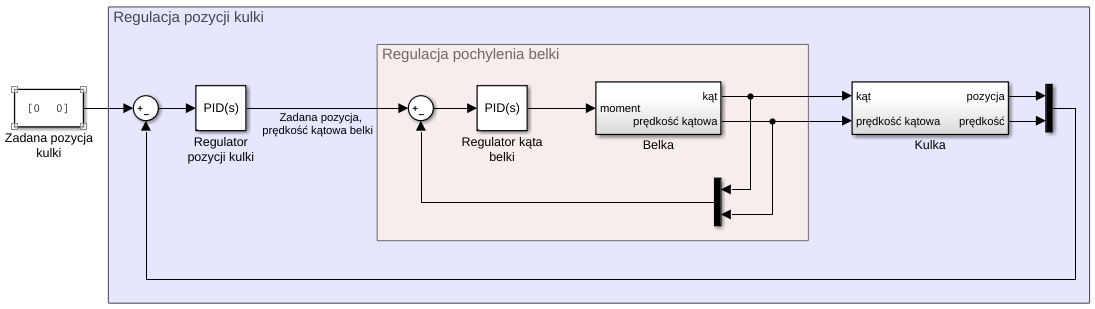
\includegraphics[width=1\textwidth]{kaskadowy_uklad_regulacji}
    \caption{Schemat ilustrujący ideę kaskadowego układu regulacji obiektu typu kulka i~belka.}
    \label{fig:kaskadowy_uklad_regulacji}
\end{figure}

\pagebreak

Aby możliwe było obliczenie osobnych regulatorów dla kulki oraz dla belki, równanie stanu powinno mieć następującą strukturę:

\begin{equation}
    \renewcommand\arraystretch{2}
    \begin{matrix}
        \text{kulka}~\Bigg\{ \\
        \text{belka}~\Bigg\{ 
    \end{matrix}
    \renewcommand\arraystretch{1}
    \left[
    \begin{array}{c}
        \bar{x}_1' \\
        \bar{x}_2' \\
        \hline
        \bar{x}_3' \\
        \bar{x}_4'
    \end{array}
    \right]
    =
    \underbrace{
        \renewcommand\arraystretch{2}
        \left[
        \begin{array}{c|c}
           \bar{A}_{11} & \bar{A}_{12} \\
           \hline
           0 & \bar{A}_{22}
        \end{array}
        \right]
    }_{\bar{A}}
    \left[
    \begin{array}{c}
        \bar{x}_1 \\
        \bar{x}_2 \\
        \hline
        \bar{x}_3 \\
        \bar{x}_4 \\
    \end{array}
    \right]
    +
    \underbrace{
        \renewcommand\arraystretch{2}
        \left[
        \begin{array}{c}
        0 \\
        \hline
        \bar{B}_2
        \end{array}
        \right]
    }_{\bar{B}}
    u \label{eq:warunki_kaskady}
\end{equation}

Z \eqref{eq:warunki_kaskady} wynika, że zachowanie kulki zależy od kulki i belki, a nie zależy od sterowania, natomiast zachowanie belki zależy tylko od belki i sterowania:

\begin{align*}
    \begin{bmatrix}
        \bar{x}_1' \\ \bar{x}_2'
    \end{bmatrix}
    &= \begin{bmatrix}
    \bar{A}_{11} & \bar{A}_{12}
    \end{bmatrix} \bar{x} \\
    \begin{bmatrix}
    \bar{x}_3' \\ \bar{x}_4'
    \end{bmatrix}
    &= \begin{bmatrix}
    0 & \bar{A}_{22}
    \end{bmatrix} \bar{x}
    + \bar{B}_2 u
\end{align*}

Jak można łatwo zauważyć, struktury macierzy $\breve{A}$ i $\breve{B}$ \eqref{eq:macierze_stanu2} nie odpowiadają strukturom pożądanych macierzy $\bar{A}$ i $\bar{B}$. Może to być spowodowane bezwładnością kulki: w momencie ruchu belki w dół, kulka pod wpływem tarcia przesuwa się odrobinę względem powierzchni belki w stronę przeciwną do kierunku spadku (ilustracja na \cref{fig:przeciwny_ruch_kulki}). Sugeruje to niewielka i ujemna zależność przyspieszenia kątowego kulki $\breve{x}_2'$ od sterowania~$u$, podczas gdy zależność belki od sterowania ma znak dodatni i dużo większy współczynnik.

\begin{figure}[h]
    \centering
    \includesvg[width=0.6\textwidth,svgpath=./vector_graphics/]{przeciwny_ruch_kulki}
    \caption{Ilustracja toczenia się kulki w przeciwną stroną niż kierunek spadku.}
    \label{fig:przeciwny_ruch_kulki}
\end{figure}

Kompensacji takiego ruchu kulki, a więc doprowadzenia macierzy $\breve{B}$ do struktury macierzy $\bar{B}$, można dokonać przez transformację $\hat{x} = T_2 \breve{x}$ zdefiniowaną jak w \eqref{eq:transformacja_x}; za macierz $T_2$ dobrano:
\begin{equation}\label{eq:transformacja2_x}
    \renewcommand\arraystretch{1.2}
    T_2 = \begin{bmatrix}
        1 & 0 & -\frac{\breve{B}_2}{\breve{B}_4} & 0 \\
        0 & 1 & 0 & -\frac{\breve{B}_2}{\breve{B}_4} \\
        0 & 0 & 1 & 0 \\
        0 & 0 & 0 & 1 \\
    \end{bmatrix}
\end{equation}
gdzie $\breve{B}_i$ oznacza \textit{i}-ty element macierzy $\breve{B}$.
% TODO: skąd się bierze ten współczynnik?!?!?!?!

Dzięki przekształceniu przez macierz \eqref{eq:transformacja2_x} otrzymano następujące macierze stanu:
\begin{align}
    \hat{A} &= \begin{bmatrix}
    0 & 1 & 0 & 0 \\
    0 & 0 & 7,0047 & 0 \\
    0 & 0 & 0 & 1 \\
    3,3914 & 0 & 0,0331 & -6,9832 \\
    \end{bmatrix}
    =
    \renewcommand\arraystretch{2}
    \left[
        \begin{array}{c|c}
        \hat{A}_{11} & \hat{A}_{12} \\
        \hline
        \hat{A}_{21} & \hat{A}_{22}
        \end{array}
    \right] \nonumber \\
    \hat{B} &= \begin{bmatrix}
    0 \\
    0 \\
    0 \\
    6,8896 \\
    \end{bmatrix} \nonumber \\
    \hat{C} &= \begin{bmatrix}
    1 & 0 & -0,0675 & 0 \\
    0 & 1 & 0 & -0,0675 \\
    0 & 0 & 1 & 0 \\
    0 & 0 & 0 & 1 \\
    \end{bmatrix} \nonumber \\
    \hat{D} &= 0 \label{eq:macierze_stanu3}
\end{align}

Widać, że postać macierzy $\hat{B}$ z \eqref{eq:macierze_stanu3} odpowiada już oczekiwanej strukturze, natomiast macierz $\hat{A}$~jeszcze nie ma takiej formy. W związku z tym zdecydowano się doprowadzić macierz $\hat{A}$ do postaci blokowo-trójkątnej górnej poprzez wyzerowanie $\hat{A}_{21}$. Nowe macierze stanu przedstawiają się następująco:
\begin{align}
    A &= \begin{bmatrix}
    0 & 1 & 0 & 0 \\
    0 & 0 & 7,0047 & 0 \\
    0 & 0 & 0 & 1 \\
    0 & 0 & 0,0331 & -6,9832 \\
    \end{bmatrix} \nonumber \\
    B &= \begin{bmatrix}
    0 \\
    0 \\
    0 \\
    6,8896 \\
    \end{bmatrix} \nonumber \\
    C &= \begin{bmatrix}
    1 & 0 & -0,0675 & 0 \\
    0 & 1 & 0 & -0,0675 \\
    0 & 0 & 1 & 0 \\
    0 & 0 & 0 & 1 \\
    \end{bmatrix} \nonumber \\
    D &= 0 \label{eq:macierze_stanu4}
\end{align}

Aby udowodnić, że wyzerowanie ww. elementu macierzy $\hat{A}$ nie przyniosło negatywnych skutków, poniżej przedstawiono wykresy charakterystyk amplitudowo-fazowych dla systemów opisanych macierzami $\hat{A}$, $\hat{B}$, $\hat{C}$ i $\hat{D}$ oraz $A$, $B$, $C$ i $D$.

Jak widać na \cref{fig:charakterystyka_amplitudowo_fazowa}, w bardzo niskich częstotliwościach (poniżej \SI{1}{\hertz}) układy nie zachowują się jednakowo. Wynika to z faktu, że przy tak powolnych ruchach belką kulka jest w stanie potoczyć się dalej od środka belki, a zatem jej oddziaływanie na belkę rośnie. Jednakże w wyższych częstotliwościach charakterystyki układów są takie same i w związku z tym można założyć, że macierze wynikowe $A$, $B$, $C$ i $D$ są poprawne.

Ostatecznie uzyskano następujące równania stanu:
\begin{align}
\begin{bmatrix}
    \dot{x}_1 \\ \dot{x}_2 \\ \dot{x}_3 \\ \dot{x}_4
\end{bmatrix}
&= \begin{bmatrix}
    0 & 1 & 0 & 0 \\
    0 & 0 & 7,0047 & 0 \\
    0 & 0 & 0 & 1 \\
    0 & 0 & 0,0331 & -6,9832
\end{bmatrix}
\begin{bmatrix}
    x_1 \\ x_2 \\ x_3 \\ x_4
\end{bmatrix}
+
\begin{bmatrix}
    0 \\ 0 \\ 0 \\ 6,8896
\end{bmatrix}
u \label{eq:rownania_stanu} \\%\displaybreak\\
\begin{bmatrix}
    y_1 \\ y_2 \\ y_3 \\ y_4
\end{bmatrix}
&= \begin{bmatrix}
    1 & 0 & -0,0675 & 0 \\
    0 & 1 & 0 & -0,0675 \\
    0 & 0 & 1 & 0 \\
    0 & 0 & 0 & 1 \\
\end{bmatrix}
\begin{bmatrix}
x_1 \\ x_2 \\ x_3 \\ x_4
\end{bmatrix} \label{eq:rownania_wyjscia} 
\end{align}

\begin{figure}[h]
    \centering
    \includesvg[width=1\textwidth,svgpath=./vector_graphics/]{ch_amplitudowo_fazowa}
    \caption{Wykresy amplitudowo-fazowe systemów opisanych macierzami \eqref{eq:macierze_stanu3} oraz \eqref{eq:macierze_stanu4}. Przedstawiona charakterystyka dla pierwszej zmiennej stanu (położenia linio\-wego kulki).}
    \label{fig:charakterystyka_amplitudowo_fazowa}
\end{figure}

Do uzyskania struktury kaskadowej systemu zlinearyzowanego należy wydzielić równania stanu kulki oraz belki:
\begin{align}
\begin{bmatrix}
\dot{x}_1 \\ \dot{x}_2
\end{bmatrix}
&= \begin{bmatrix}
    0 & 1 & 0 \\
    0 & 0 & 7,0047
\end{bmatrix}
\begin{bmatrix}
    x_1 \\ x_2 \\ x_3
\end{bmatrix} \label{eq:rownania_stanu_kulki} \\
\begin{bmatrix}
    y_1 \\ y_2
\end{bmatrix}
&= \begin{bmatrix}
    1 & 0 & -0,0675 & 0 \\
    0 & 1 & 0 & -0.0675 \\
\end{bmatrix}
\begin{bmatrix}
x_1 \\ x_2 \\ x_3 \\ x_4
\end{bmatrix} \label{eq:rownania_wyjscia_kulki} \\
\begin{bmatrix}
    \dot{x}_3 \\ \dot{x}_4
\end{bmatrix}
&= \begin{bmatrix}
    0 & 1 \\
    0,0331 & -6,9832
\end{bmatrix}
\begin{bmatrix}
    x_3 \\ x_4
\end{bmatrix}
+
\begin{bmatrix}
    0 \\ 6,8896
\end{bmatrix}
u \label{eq:rownania_stanu_belki} \\%\displaybreak\\
\begin{bmatrix}
    y_3 \\ y_4
\end{bmatrix}
&= \begin{bmatrix}
    1 & 0 \\
    0 & 1 \\
\end{bmatrix}
\begin{bmatrix}
    x_3 \\ x_4
\end{bmatrix} \label{eq:rownania_wyjscia_belki} 
\end{align}

Oczywiście taka forma równań \eqref{eq:rownania_stanu_kulki} i \eqref{eq:rownania_wyjscia_kulki} jest niepoprawna, ale bardzo łatwo można ją przekształcić do schematu z \cref{fig:kaskadowy_uklad_regulacji} stosując podmianę $u_1^* = x_3$, $u_2^* = x_4$: %(równania \eqref{eq:rownania_stanu_kulki2} oraz \eqref{eq:rownania_wyjscia_kulki2}). 
\begin{align}
\begin{bmatrix}
    \dot{x}_1 \\ \dot{x}_2
\end{bmatrix}
&= \begin{bmatrix}
    0 & 1 \\
    0 & 0
\end{bmatrix}
\begin{bmatrix}
x_1 \\ x_2
\end{bmatrix}
+
\begin{bmatrix}
    0 & 0 \\ 7,0047 & 0
\end{bmatrix}
\begin{bmatrix}
    u_1^* \\ u_2^*
\end{bmatrix} \label{eq:rownania_stanu_kulki2} \\
\begin{bmatrix}
    y_1 \\ y_2
\end{bmatrix}
&= \begin{bmatrix}
    1 & 0 \\
    0 & 1 \\
\end{bmatrix}
\begin{bmatrix}
    x_1 \\ x_2
\end{bmatrix}
+ \begin{bmatrix}
    -0,0675 & 0 \\
    0 & -0.0675
\end{bmatrix}
\begin{bmatrix}
    u_1^* \\ u_2^*
\end{bmatrix} \label{eq:rownania_wyjscia_kulki2}
\end{align}

%%%%
\section{Regulator pochylenia belki}
\label{sec:ch6_regulator_belki}

Jako regulator pochylenia belki wybrano prosty regulator proporcjonalny od stanu. Struktura regulacji przedstawiona jest na \cref{fig:schemat_regulacji_belka}, gdzie:
\begin{itemize}
    \item $\alpha_\text{ref}$ oraz $\omega_\text{ref}$ są wartościami zadanymi odpowiednio kąta oraz prędkości kątowej belki,
    \item $K_b$ jest macierzą wzmocnień regulatora,
    \item $G_b(s)$ jest transmitancją (typu \textit{SIMO}) zlinearyzowanego systemu belki opartego o równania stanu \eqref{eq:rownania_stanu_belki} i wyjścia \eqref{eq:rownania_wyjscia_belki},
    \item $y_3$, $y_4$ są wartościami wyjściowymi z modelu (pozycją kątową i prędkością kątową belki).
\end{itemize}

\begin{figure}[ht]
    \centering
    
    \begin{tikzpicture}[auto, node distance=1cm,>=latex']
        \node [input, name=input] {};
        \node [sum, right=2of input] (sum) {};
        \node [gain, right=of sum] (controller) {$K_b$};
        \node [block, right=of controller] (plant) {$G_b(s)$};
        \node [output, right=of plant] (output) {};
        \draw [draw,->] (input) -- node {$\left[\alpha_\text{ref}, ~\omega_\text{ref}\right]^\intercal$} (sum);
        \draw [->] (sum) -- node {} (controller);
        \draw [->] (controller) -- node {} (plant);
        \draw [->] (plant) -- node [name=y] {$\left[y_3, ~y_4\right]^\intercal$}(output);
        \draw [->] (y) -- ++ (0,-1.5) -| node [pos=0.95] {$-$} (sum);
    \end{tikzpicture}
    
    \caption{Schemat sterowania zlinearyzowanego systemu odpowiadającego za zachowanie belki.}
    \label{fig:schemat_regulacji_belka}
\end{figure}

Wartość wzmocnienia $K_b$ została dobrana za pomocą funkcji \texttt{looptune} z programu \textsc{Matlab}, co pozwoliło uzyskać dużą dynamikę działania regulatora. Wspomniana funkcja optymalizuje pętlę sprzężenia zwrotnego układu zaprezentowaną na \cref{fig:schemat_regulacji_looptune} według ustalonych kryteriów częstotliwościowych: \begin{itemize}
    \item pasmo przenoszenia -- punkt przejścia charakterystyki amplitudy przez zero musi zawierać się w wyznaczonym zakresie częstotliwości,
    \item wydajność -- akcja całkująca na częstotliwościach poniżej wyznaczonego zakresu,
    \item odporność (ang. \textit{robustness}) -- odpowiednie zapasy stabilności na częstotliwościach poniżej wyznaczonego zakresu.
\end{itemize}

Do funkcji \texttt{looptune} podano jako argument zakres częstotliwości \SIrange{5}{20}{\hertz}, uzyskując wzmocnienie regulatora $K_b = \left[-8,2069;~  -1,5756\right]$. Informacje o sposobie implementacji regulatora zamieszczone są w rozdziale \ref{subsec:ch7_regulator_belki}.

\begin{figure}[ht]
    \centering
    
    \begin{tikzpicture}[auto, node distance=1cm,>=latex']
    \node [block] (plant) {$G(s)$};
    \node [block, below=of plant] (controller) {$C(s)$};
    \draw [->] (plant.east) -- ++ (1,0) |- node {$y$} (controller.east);
    \draw [->] (controller.west) -- ++ (-1,0) |- node {$u$} (plant.west);
    %\draw [->] (y) -- ++ (0,-1.5) -| node [pos=0.95] {$-$} (sum);
    \end{tikzpicture}
    
    \caption{Schemat układu optymalizowanego przez funkcję \texttt{looptune}.}
    \label{fig:schemat_regulacji_looptune}
\end{figure}

% TODO: charakterystyka bodego? :(

%%%%
\section{Regulator pozycji kulki}
\label{sec:ch6_regulator_kulki}

% TODO: regulator od stanu

%%%%
\section{Podsumowanie}

% TODO: dokończ

%---------------------------------------------------------------------------
\chapter{Algorytmy sterowania}
\label{cha:ch7_algorytmy_sterowania}

Lorem ipsum.

% TODO: schemat ogólny sterowania, tj. od czego zaczynamy (od bazowania) i co robimy gdy jakieś zdarzenie wystąpi

% TODO: również schemat wywoływanych funkcji, tj. np. najpierw odczyt czujników itd.

%%%%
\section{Wykrywanie braku kulki}
\label{sec:ch7_wykrywanie_braku_kulki}

% TODO: opisz wartości progowe
% TODO: opisz zachowanie algorytmu zatrzaskiwania (histereza?)
% TODO: dodaj wykres charakterystyki czujników

%%%%
\section{Bazowanie}
\label{sec:ch7_bazowanie}

% TODO: opisz ideę
% TODO: schemat blokowy algorytmu
% TODO: wartość enkodera

%%%%
\section{Regulatory}
\label{sec:ch7_regulatory}

% TODO: ogólnie opisać sposób implementacji regulatorów w sterowniku
%---------------------------------------------------------------------------
\chapter{Algorytmy samostrojenia}
\label{cha:ch8_algorytmy_samostrojenia}

W literaturze do teorii sterowania znajdują się opisy wielu klasycznych metod strojenia regulatorów, takich jak metoda Zieglera-Nicholsa \cite{KOWAL}\cite{CTRLENG} czy Åströma-Hägglunda \cite{CTRLENG}\cite{ASTROMHAGGLUND}. Wielu producentów oprogramowania serwonapędów lub sterowników technologicznych dostarcza własne algorytmy strojenia \textit{online} \cite{S7MANUAL}\cite{SCL_S71200_S71500}.

Zdecydowano się zrezygnować z metod klasycznych strojenia algorytmów, gdyż są one powszechnie znane i polegają na doprowadzeniu obiektu do cyklu granicznego, co w przypadku zastosowanej konstrukcji przeniesienia napędu można uzyskać podając stałe sterowanie na silnik. Prawdopodobnie dokładnie z takiego powodu oprogramowanie służące do programowania sterownika PLC --- \textsc{Siemens TIA Portal} --- nie było w stanie zakończyć poprawnie procesu samostrojenia regulatora pozycji belki.

Biorąc pod uwagę powyższe ograniczenia, zdecydowano się oprzeć samostrojenie regulatorów podrzędnego i nadrzędnego o automatyczne procesy identyfikacji matematycznych obiektów belki oraz kulki, co zostało opisane w niniejszym rozdziale.

%%%%
\section{Identyfikacja obiektu belki}
\label{sec:ch8_identyfikacja_belki}

Identyfikację belki oparto o odpowiedź skokową modelu obiektu pierwszego rzędu opisanego transmitancją:
\begin{equation}
    G_b(s) = \frac{K_b}{T_b s+1}
    \label{eq:transmitancja_obiektu_pierwszego_rzedu}
\end{equation}
gdzie $K_b$ oznacza wzmocnienie obiektu, a $T_b$ jego stałą czasową (\cite{KOWAL}). Parametry te można odczytać z~wykresu odpowiedzi skokowej (\cref{fig:odpowiedz_skokowa_obiektu_pierwszego_rzedu}, równanie \eqref{eq:odpowiedz_skokowa}) obiektu w następujący sposób:
\begin{itemize}
    \item wzmocnienie $K_b$ to iloraz wartości ustalonej $h_{ss}$ oraz zadanej amplitudy $A_\text{ref}$,
    \item stała czasowa $T_b$ równa jest ilorazowi pola powierzchni $S^+$ pod asymptotą i nad wykresem charakterystyki oraz wartości ustalonej.
\end{itemize}

\begin{equation}
    h(t) = h_{ss} \left( 1 - e^{-\frac{t}{T_b}} \right) \label{eq:odpowiedz_skokowa}
\end{equation}

Pole powierzchni $S^+$ (zobrazowane na \cref{fig:odpowiedz_skokowa_obiektu_pierwszego_rzedu}) określa się jako całkę:
\begin{nalign}
    S^+ &= \int \limits_{0}^{\infty} \left(h_{ss} - h(t) \right) \mathrm{d}x \\
        &= \int \limits_{0}^{\infty} \left(K_b A_\text{ref} - K_b A_\text{ref} + K_b A_\text{ref} e^{-\frac{t}{T_b}} \right) \mathrm{d}x \\
        &= T_b K_b A_\text{ref} e^{-\frac{t}{T_b}}|_{t=0}^{\infty} \\
        &= T_b K_b A_\text{ref} \label{eq:pole_nad_figura}
\end{nalign}

Przykładową odpowiedź skokową wału motoreduktora wraz z jej aproksymacją zaprezentowano na \cref{fig:identyfikacja_belki}. W celu identyfikacji zdecydowano się wykorzystać odczyt prędkości wału motoreduktora z~dwóch powodów:
\begin{itemize}
    \item po pierwsze, tylko prędkość kątowa wału jest wartością zachowującą się ściśle jak obiekt inercyjny pierwszego rzędu,
    \item po drugie, obrót belki zależny jest sinusoidalnie od obrotu wału silnika; stąd trudniejsze byłoby odczytanie parametrów ,,ukrytych'' w przebiegu sinusoidalnym, gdyby identyfikację przeprowadzano na kącie lub prędkości kątowej belki.
\end{itemize}
Algorytm identyfikacyjny (zob. rozdział \ref{sec:ch8_algorytm_identyfikacji_belki}) również korzysta z odpowiedzi skokowej wału motoreduktora.

\begin{figure}[ht]
    \centering
    \begin{tikzpicture}
        \begin{axis}[
            domain=0.0:3,
            xmin=0, xmax=2,
            ymin=0, ymax=40,
            samples=400,
            axis y line=center,
            axis x line=middle,
            legend pos=north west,
        ]
            \addplot+[name path=A, no marks] {25*(1-e^(-x/0.118))};
            \addlegendentry{Odpowiedź skokowa $h(t)$};
            \addplot[dashed,name path=B] {25};
            \addlegendentry{Wartość graniczna (stan ustalony) $h_{ss}$};
            \addplot[pattern=north east lines,pattern color=gray] fill between[of=A and B];
            \addlegendentry{Pole nad odpowiedzią skokową $S^+$};
        \end{axis}
    \end{tikzpicture}
    \caption{Wykres odpowiedzi skokowej obiektu inercyjnego pierwszego rzędu.}
    \label{fig:odpowiedz_skokowa_obiektu_pierwszego_rzedu}
\end{figure}

\begin{figure}[ht]
    \centering
    \includesvg[width=1\textwidth,svgpath=./vector_graphics/]{identyfikacja_belki}    
    \caption{Przykład aproksymacji odpowiedzi skokowej prędkości obrotowej wału motoreduktora.}
    \label{fig:identyfikacja_belki}
\end{figure}

Należy zwrócić uwagę, że wartością, która częściej jest wykorzystywana w algorytmach sterowania w tym obiekcie, jest nie prędkość kątowa wału motoreduktora, ale jego pozycja kątowa. Rozważany w procesie identyfikacji obiekt \eqref{eq:transmitancja_obiektu_pierwszego_rzedu} nie reprezentuje odpowiedzi kątowej silnika, dlatego należy użyć dodatkowego integratora, co pozwoli uzyskać kąt obrotu:
\begin{equation}
    H_b(s) = G_b(s) \cdot \frac{1}{s} = \frac{K_b}{T_b s^2 + s} \label{eq:transmitancja_silnik_odp_katowa}
\end{equation}

Obiektowi w ten sposób opisanemu odpowiadają następujące macierze stanu\footnote{Dzięki użyciu charakterystyki obiektu całkującego rzeczywistego \eqref{eq:transmitancja_silnik_odp_katowa} możliwe jest rozszerzenie macierzy wyjścia tak, aby móc odczytać dwa stany jednocześnie; nie jest to jednak wymagane w dalszej analizie, dlatego zostało pominięte.}:
\begin{nalign}
    A_I &= \begin{bmatrix}
        0 & 1 \\ 0 & -\frac{1}{T_b}
    \end{bmatrix} \\
    B_I &= \begin{bmatrix}
        0 \\ \frac{K_b}{T_b}
    \end{bmatrix} \\
    C_I &= \begin{bmatrix}
        1 & 0
    \end{bmatrix} \\
    D_I &= 0  \label{eq:macierze_stanu_obiektu_pierwszego_rzedu}
\end{nalign}

Regulator, który steruje belką, oparty jest o stan (kąt i prędkość kątową obrotu) belki (zob. rozdział \ref{sec:ch6_regulator_belki}), a jego nastawy obliczono wykorzystując funkcję \texttt{looptune} z programu \textsc{Matlab}, która optymalizuje zadany układ w dziedzinie częstotliwości. Przy samostrojeniu tego regulatora zdecydowano się na inne podejście oparte o przesuwanie wartości własnych zamkniętego układu. W tym celu wyliczono zależność algebraiczną pomiędzy nastawami regulatora a zadanymi wartościami własnymi.

Zamknięty układ regulacji z regulatorem od stanu $K_I = \begin{bmatrix}
    k_1 & k_2
\end{bmatrix}$ opisany jest równaniem:
\begin{equation}
    x' = \underbrace{(A_I - B_I K_I)}_{M \in \mathbb{C}^{2 \times 2}} x
\end{equation}

Macierz $M$ ma dwie wartości własne $\lambda_1$ oraz $\lambda_2$, które spełniają następujące zależności:
\begin{nalign}
    \det(M) &= \lambda_1 \lambda_2 \\
    \tr(M) &= \lambda_1 + \lambda_2 \label{eq:obiekt1_zaleznosc_lambd}
\end{nalign}

Dzięki \eqref{eq:obiekt1_zaleznosc_lambd} możliwe jest uzyskanie układu równań, po którego rozwiązaniu uzyskuje się następującą zależność na $K_I$:

\begin{nalign}
    k_1 &= \frac{\lambda_1 \lambda_2}{\frac{K_b}{T_b}} \\
    k_2 &= \frac{\frac{-1}{T_b} - \lambda_1 - \lambda_2}{\frac{K_b}{T_b}} \label{eq:zaleznosc_regulator_belki}
\end{nalign}

Należy zwrócić uwagę, że postać równań stanu obiektu \eqref{eq:macierze_stanu_obiektu_pierwszego_rzedu} nie do końca odpowiada postaci otrzymanej z linearyzacji \eqref{eq:rownania_stanu_belki} i \eqref{eq:rownania_wyjscia_belki}, w związku z tym zdecydowano się narzucić inne wartości własne macierzy $M$ niż te, które ma ,,zwinięty'' układ regulatora pozycji belki (\cref{fig:schemat_regulacji_belka}).

% TODO: inne wartości własne

%%%%
\section{Algorytm identyfikacji obiektu belki}
\label{sec:ch8_algorytm_identyfikacji_belki}

Opisany w rozdziale \ref{sec:ch8_identyfikacja_belki} eksperyment (odpowiedź skokowa prędkości kątowej wału motoreduktora) został zaimplementowany w sterowniku PLC, a jego wyniki służą do obliczania nowych nastaw regulatora według równań \eqref{eq:zaleznosc_regulator_belki}. Eksperyment polega na ustawieniu sterowania silnika na \SI{50}{\percent} na czas \SI{2}{\second}~i~zarejestrowaniu odczytu prędkości kątowej wału motoreduktora (jego odpowiedzi skokowej).

Procedura identyfikacyjna została przeprowadzona w sekwencji opisanej na \cref{fig:schemat_samostrojenia_belka}, a sama sekwencja została zaimplementowana w języku drabinkowym \textit{LAD} podobnie jak sekwencja bazowania czy sekwencja główna (rozdział \ref{sec:sekwencja_glowna}).

\begin{figure}[ht]
    \centering
    
    \begin{tikzpicture}[auto, node distance=1cm,>=latex']
    \node [startblock] (S1) {Reset zapisanych wartości};
    \node [block, below=2of S1] (S2) {Obliczanie całki pod wykresem};
    \node [block, right=of S2] (S3) {Zbieranie danych do obliczenia $h_{ss}$};
    \node [block, below=2of S2] (S4) {Obliczanie parametrów};
    \node [block, below=of S4] (S5) {Obliczanie regulatora};
        
    \draw [->] (S1) -- node [name=J1,left] {} node[name=T1,pos=0.75] {$T_1$} (S2);
    \draw [->] (J1) -| node [name=T2,pos=0.75] {$T_2$} (S3.north);
    \draw [->] (S2) -- node [name=J2,left] {} node[name=T3,pos=0.75] {$T_3$} (S4);
    \draw [-] (S3) |- (J2);
    \draw [->] (S4) -- (S5);
    \end{tikzpicture}
    
    \caption{Schemat sekwencji samostrojenia regulatora belki.}
    \label{fig:schemat_samostrojenia_belka}
\end{figure}

Tranzycjom $T_i$ zaznaczonym na schemacie na \cref{fig:schemat_samostrojenia_belka} odpowiadają następujące warunki:
\begin{itemize}
    \item $T_1$ -- rozpoczęcie eksperymentu (podanie sterowania \SI{50}{\percent} na silnik),
    \item $T_2$ -- upłynięcie czasu połowy eksperymentu (\SI{1}{\second}),
    \item $T_3$ -- zakończenie eksperymentu.
\end{itemize}

Krok pierwszy algorytmu, oznaczony jako \textit{Reset zapisanych wartości}, zeruje zapisaną wartość całki oraz dwa rejestry przechowujące sumę oraz ilość wartości, co uaktualniane jest co cykl procesora w~bloku \textit{Zbieranie danych do obliczenia $h_{ss}$}. Wartości te służą do obliczenia średniej arytmetycznej, która odpowiada oczekiwanej wartości ustalonej prędkości $h_{ss}$. Jest to wymuszone mocną kwantyzacją chwilowych wartości prędkości, co można zaobserwować na \cref{fig:identyfikacja_belki}.

Obliczanie całki odbywa się za pomocą bloku \texttt{LGF\_Integration}\cite{LGF} dostępnego w bibliotece \texttt{LGF} udostępnionej przez firmę \textsc{Siemens}. Na podstawie wzorów umieszczonych w rozdziale \ref{sec:ch8_identyfikacja_belki} obliczane są parametry $S$ (pole całkowite), $A_b$, $K_b$, $S^+$, $T_b$ oraz nastawy regulatora $k_1$, $k_2$.

%%%%
\section{Identyfikacja obiektu kulki}
\label{sec:ch8_identyfikacja_kulki}

Wykorzystując schemat sił działających na kulkę znajdującą się na pochylonej pod kątem $\theta$ belce (\cref{fig:sily_dzialajace_na_kulke}) wyznaczono, w sposób opisany poniżej, zależność przyspieszenia liniowego, które działa na kulkę, od kąta pochylenia belki.

\def\iangle{6} % Angle of the inclined plane
\def\arcr{1.1cm} % Radius of the arc used to indicate angles
\def\down{-90}

\begin{figure}[ht]
    \centering
    \begin{tikzpicture}[
        scale = 3,
        force/.style={>=latex,draw=blue,fill=blue},
        plane/.style={draw=black},
        M/.style={draw,circle,fill=lightgray,minimum size=1cm,thin},
        axis/.style={densely dashed,gray,font=\small},
    ]
        %\draw[plane] (0,-) coordinate (base) 
        %-- coordinate[pos=0.5] (mid) ++(\iangle:3) coordinate (top)
        %|- (base) -- cycle;
        \draw[dashed] (3,-1) -- (0,-1) coordinate (base);
        \draw (base)
        -- coordinate[pos=0.5] (mid) ++(\iangle:3) coordinate (top);
        \path (mid) node[M,rotate=\iangle,yshift=0.5cm] (M) {};
        \draw[->] (base)++(\arcr,0) arc (0:\iangle:\arcr);
        \path (base)++(\iangle*0.5:\arcr+3pt) node {$\theta$};
        
        \begin{scope}[rotate=\iangle]
            \draw [force,->] (M.center) -- ++(0,0.4) node[above right] {$\vec{N}$};
            % Assuming that Mg = 1. The normal force will therefore be cos(alpha)
            \draw [force,->] (M.west) -- ++(-0.3,0) node[above] {$\vec{F_1}$};
            \draw [force,->] (M.south) -- ++(0.3,0) node[above] {$\vec{N_1}$};
        \end{scope}
        \draw[force,->] (M.center) -- ++(0,-0.4) node[below] {$\vec{Q}$};
    \end{tikzpicture}
    
    \caption{Schemat sił działających na kulkę znajdującą się na pochylonej pod kątem $\theta$ belce.}
    \label{fig:sily_dzialajace_na_kulke}
\end{figure}

Zgodnie z rysunkiem, na kulkę działają dwie siły: $\vec{Q}$ (siła ciężkości) i $\vec{N}$ (siła reakcji podłoża). Dodatkowo zostały zaznaczone składowe równoległe do powierzchni belki wspomnianych sił, $\vec{F_1}$ oraz $\vec{N_1}$; ich wypadkowa $F = am = F_1 - N_1$ jest siłą powodującą staczanie się kulki z przyspieszeniem wypadkowym $a$ wzdłuż belki.

Wartość siły ciężkości działającej na kulkę definiowana jest jako $Q=mg$, gdzie $m$ to masa kulki, a~$g$~to przyspieszenie ziemskie. Automatycznie składowa $F_1$ ma wartość $F_1=mg\sin\theta$.

Siła $\vec{N_1}$, pochodząca od tarcia suchego kulki o belkę, wprowadza kulkę w ruch obrotowy, stąd $\epsilon J = r N_1$, gdzie $\epsilon$ to przyspieszenie kątowe kulki, $J$ to moment bezwładności kulki, a $r$ to jej promień. Dodatkowo pojawia się zależność przyspieszenia liniowego od kątowego $a = \epsilon r$, która jest właściwa przy braku poślizgu kulki o belkę.

Podstawiając wartości sił $F_1$ i $N_1$ do równania na siłę wypadkową działającą na kulkę otrzymano:

\begin{nalign}
    F &= mg\sin\theta - \frac{\epsilon}{r}J \\
    a m &= mg\sin\theta - \frac{a}{r^2}J \\
    a\left(m + \frac{J}{r^2} \right) &= mg\sin\theta \\
    a &= \frac{mg\sin\theta}{m+\frac{J}{r^2}} \\
      &= \frac{r^2mg\sin\theta}{r^2m+J}
    \label{eq:przyspieszenie_kulki1}
\end{nalign}

Wiadomo, że moment bezwładności $J$ jednolitej kulki o promieniu $r$ wynosi $J=\frac{2}{5}r^2m$. Podstawiając ten wzór do wyniku z \eqref{eq:przyspieszenie_kulki1} otrzymano:

\begin{nalign}
    a &= \frac{r^2mg\sin\theta}{r^2m+J}\\
      &= \frac{r^2mg\sin\theta}{r^2m+\frac{2}{5}r^2m} \\
      &= \frac{g\sin\theta}{1+\frac{2}{5}} \\
      &= \frac{5}{7} g \sin\theta
    \label{eq:przyspieszenie_kulki2}
\end{nalign}

Wartość $\frac{5}{7}g$ to w przybliżeniu 7, natomiast dla małych kątów $\sin\theta \approx \theta$. Stąd ostateczny wynik:

\begin{equation}
    a \approx 7 \cdot \theta \label{eq:przyspieszenie_kulki3}
\end{equation}

Oznacza to, że przyspieszenie kulki staczającej się po pochylonej belce jest stałe i wynosi około siedmiokrotność kąta pochylenia belki. Należy w tym miejscu zwrócić uwagę na wyniki linearyzacji \eqref{eq:rownania_stanu_kulki2} oraz \eqref{eq:rownania_wyjscia_kulki2}, które zostały przypomniane poniżej:

\begin{align*}
    \begin{bmatrix}
        \dot{x}_1 \\ \dot{x}_2
    \end{bmatrix}
    &= \begin{bmatrix}
        0 & 1 \\
        0 & 0
    \end{bmatrix}
    \begin{bmatrix}
        x_1 \\ x_2
    \end{bmatrix}
    +
    \begin{bmatrix}
        0 & 0 \\ 7,0047 & 0
    \end{bmatrix}
    \begin{bmatrix}
        u_1^* \\ u_2^*
    \end{bmatrix}\\
    \begin{bmatrix}
        y_1 \\ y_2
    \end{bmatrix}
    &= \begin{bmatrix}
        1 & 0 \\
        0 & 1 \\
    \end{bmatrix}
    \begin{bmatrix}
        x_1 \\ x_2
    \end{bmatrix}
    + \begin{bmatrix}
        -0,0675 & 0 \\
        0 & -0.0675
    \end{bmatrix}
    \begin{bmatrix}
        u_1^* \\ u_2^*
    \end{bmatrix}
\end{align*}

Jak widać po równaniach stanu, $x_1$ jest całką $x_2$, a pochodna stanu $x_2$ --- $\dot{x}_2$ --- jest siedmiokrotnością sterowania $u_1^*$. Wyniki te są zgodne z otrzymaną zależnością \eqref{eq:przyspieszenie_kulki3}, gdyż $x_1$ to pozycja liniowa kulki, $x_2$ to jej prędkość liniowa, $\dot{x}_2$ to przyspieszenie liniowe, a $u_1^*$ to kąt belki.

Powyższy wywód dowodzi, że przyspieszenie kulki, które charakteryzuje jej dynamikę, jest niezależne od momentu bezwładności kulki --- czyli od jej masy i rozmiaru --- a~zatem eksperymenty identyfikacyjne (takie jak pomiar czasu i/lub drogi staczania się kulki) nie dadzą rezultatów, które mogłyby w jakikolwiek sposób pomóc w doborze regulatora.

Regulator nadrzędny został zbudowany dla systemu ,,zwiniętego'' (zob. rozdział \ref{sec:ch6_regulator_kulki}), obejmującego wewnętrzną pętlę sprzężenia zwrotnego dla systemu belki oraz system kulki, a zatem po zmianie parametrów tej pętli wewnętrznej można ponownie przeprowadzić obliczenia dające nowe nastawy regulatora nadrzędnego. Po przeprowadzeniu takich obliczeń z wykorzystaniem funkcji \texttt{looptune} okazało się, że ,,nowe'' nastawy są zbliżone do nastaw regulatora dla modelu zlinearyzowanego, dlatego zdecydowano się pominąć te obliczenia w procesie samostrojenia.

%%%%
\section{Podsumowanie}

W niniejszym rozdziale zaprezentowano metodę samostrojenia regulatora podrzędnego opartą o identyfikację modelu matematycznego obiektu inercyjnego pierwszego rzędu, jakim jest silnik użyty w obiekcie regulacji. Opisano również matematyczne zależności między parametrami takiego modelu a jego odpowiedzią skokową. Następnie przeprowadzono obliczenia zależności pomiędzy regulatorem od stanu, obiektem inercyjnym pierwszego rzędu oraz zadanymi wartościami własnymi układu z zamkniętą pętlą sprzężenia zwrotnego. W kolejnej części rozdziału opisano implementację procedury samostrojenia, wykorzystującą zależności parametrów obiektu i odpowiedzi skokowej, na sterowniku PLC.

Na koniec przeprowadzono wywód udowadniający, że przeprowadzona identyfikacja kulki nie powiedzie się, gdyż jej model liniowy jest niezależny od parametrów fizycznych kulki, a jedynie od kąta obrotu belki. Z tego powodu zaniechano implementacji procedury samostrojenia dla kulki.

%---------------------------------------------------------------------------
\chapter{Symulacje i eksperymenty}
\label{cha:ch9_symulacje_i_eksperymenty}

Aby sprawdzić poprawność działania modelów nieliniowego i liniowego (rozdział \ref{sec:ch6_punkt_pracy_linearyzacja}) obiektu przeprowadzono szereg opisanych w tym rozdziale symulacji. Sprawdzono również działanie regulatorów zaimplementowanych w rzeczywistym obiekcie regulacji, a także porównano wynik działania regulatorów dobranych matematycznie (rozdziały \ref{sec:ch6_regulator_belki} oraz \ref{sec:ch6_regulator_kulki}) z regulatorem dostrojonym w procedurze samostrojenia (rozdział \ref{cha:ch8_algorytmy_samostrojenia}).

%%%%
\section{Symulacje modelów}
\label{sec:ch9_symulacje_modelow}

% TODO: symulacja modelu nieliniowego i liniowego no chyba że nie wyjdzie

%%%%
\section{Symulacje działania regulatorów}
\label{sec:ch9_symulacje_regulatorow}

% TODO: symulacje regulatorów na modelu nieliniowym i liniowym

%%%%
\section{Eksperymenty przeprowadzone na obiekcie rzeczywistym}
\label{sec:ch9_eksperymenty}

%%%%
\subsection{Stabilizacja położenia różnych kulek}
\label{subsec:ch9_stabilizacja_polozenia_roznych_kulek}

%%%%
\subsection{Odpowiedź regulatora belki przed i po samostrojeniu}
\label{subsec:ch9_odp_regulatora_belki}

%%%%
\subsection{Stabilizacja położenia różnych kulek po samostrojeniu regulatora belki}
\label{subsec:ch9_stabilizacja_polozenia_roznych_kulek_po_samostrojeniu}

%%%%
\section{Podsumowanie}

%%%%
% pomysły na eksperymenty:
% - nastrojony przez autotune'a w TIA Portal regulator PID - umiejętność stabilizacji kulki piankowej
% - jw. zmiana kulki na piłkę tenisową bez przeprowadzania autotune'a
% - jw. ale po przeprowadzeniu autotune'a
% - regulatory od stanu obliczone analitycznie (kulka piankowa)
% - regulatory od stanu obliczone analitycznie (piłka tenisowa)
% - samostrojenie z kulką piankową i rezultaty
% - jw. z piłką tenisową i rezultaty
% - przestrojenie na piłkę tenisową i rezultaty

% do tego symulacje:
% - porównanie zachowania modelu nieliniowego i liniowego
% - porównanie zachowania modelu liniowego i rzeczywistego
% - porównanie zachowania modelu nieliniowego i rzeczywistego

%---------------------------------------------------------------------------
\chapter{Wnioski i podsumowanie pracy}
\label{cha:ch10_wnioski}

% zrealizowane zagadnienia
W niniejszej pracy zrealizowano następujące zagadnienia:
\begin{itemize}
    \item budowa od podstaw obiektu regulacji,
    \item dobór czujników i oprzyrządowania,
    \item stworzenie nieliniowego modelu symulacyjnego na podstawie rzeczywistego obiektu,
    \item przeprowadzenie identyfikacji charakterystyk nieliniowych czujników i parametrów wykorzystanego silnika prądu stałego,
    \item zaproponowanie kaskadowego układu regulacji i linearyzacja modelu nieliniowego,
    \item przekształcenie modelu liniowego do postaci wymaganej przez kaskadowy układ regulacji,
    \item synteza regulatorów,
    \item implementacja algorytmów sterowania w sterowniku PLC,
    \item zaproponowanie metody samostrojenia regulatora podrzędnego bazującej na procedurze identyfikacji obiektu inercyjnego pierwszego rzędu,
    \item zaprogramowanie wspomnianej metody samostrojenia,
    \item przeprowadzenie symulacji wykazujących odpowiednie zachowanie modelu liniowego i nieliniowego obiektu,
    \item przeprowadzenie eksperymentów porównujących zachowanie obiektu regulacji dla różnych kulek,
    \item przeprowadzenie eksperymentów porównujących odpowiedzi regulatora podrzędnego przed i po samostrojeniu,
    \item przeprowadzenie kolejnych eksperymentów porównujących jakość stabilizacji pozycji kulki w~obiekcie po samostrojeniu i przy wykorzystaniu różnych kulek.
\end{itemize}

Spośród założonych celów, opisanych we wstępie do pracy (rozdział \ref{cha:ch1_wstep}), niemożliwym i niecelowym było przeprowadzenie samostrojenia regulatorów opartego o identyfikację dynamiki kulki, na co dowód zamieszczono w rozdziale \ref{sec:ch8_identyfikacja_kulki}. Udało się natomiast dobrać naturalną strukturę sterowania, w której następuje dekompozycja układów regulacji: każdy odpowiada tylko za swoje ograniczone pole działania; przykładowo: jeżeli zachowanie kulki zależy przede wszystkim od kąta belki (\ref{sec:ch8_identyfikacja_kulki}), to regulator pozycji kulki powinien wymuszać odpowiednie ustawienie belki dla pożądanej odpowiedzi kulki.

%Ponadto należy wspomnieć, że implementacja układu sterowania, wraz z dodatkowymi działaniami jak na przykład implem

\section{Podsumowanie wyników}

Zaproponowany układ sterowania naturalnie oddziela role regulatorów, co zostało zasygnalizowane wcześniej w tym rozdziale. Implementacja regulatorów proporcjonalnych od stanu pozwala spełniać główne zadanie regulacji --- stabilizować kulkę w zerowym położeniu --- w sposób odpowiednio szybki.

Na podstawie wyników symulacji modelu nieliniowego oraz niektórych eksperymentów można wyciągnąć wniosek, że w pewnych sytuacjach może wystąpić uchyb statyczny regulacji --- głównie na skutek obecności tarcia statycznego kulki lub nieregularności w jej budowie (np. szwy) --- co oznacza, że rozsądnym byłoby rozbudowanie regulatora nadrzędnego o akcję całkującą, mającą za zadanie zminimalizować wspomniany uchyb.

Należy również wspomnieć o przydatności wykorzystanych do budowy układu sterowania narzędzi inżynieryjnych oferowanych przez pakiet \textsc{Matlab/Simulink}. Bardzo dużym uproszczeniem w~stosunku do ,,klasycznych'' metod modelowania (np. równań Eulera-Lagrange'a) było wykorzystanie przybornika narzędziowego \textsc{Simscape Multibody}, który umożliwił zbudowanie wirtualnego obiektu regulacji na podstawie fizycznych parametrów rzeczywistego układu, istniejących w nim połączeń i mas poszczególnych elementów. Spośród użytych narzędzi, funkcja \texttt{looptune} jako jedyna zaprezentowała mieszane wyniki; z jednej strony, regulator pozycji belki zbudowany przy jej użyciu działał bardzo dobrze, z drugiej strony nie poradziła sobie z syntezą regulatora nadrzędnego (rozdział \ref{sec:ch6_regulator_kulki}; wymagane było zmienienie dwóch wzmocnień). Należy mieć na uwadze, że funkcja \texttt{looptune} ma charakter optymalizacyjny, a więc być może jej wartości początkowe były nieodpowiednie; być może jednak problem stanowiły zaszumione sygnały z czujników położenia kulki, co skutkowało dużymi skokami wartości prędkości kulki. Dodatkowy negatywny wpływ na działanie regulatora obliczonego przez wspomnianą funkcję mógł mieć błąd wynikający z obliczania prędkości kulki i belki na zasadzie równań różnicowych z określonym okresem.

% wnioski
% Wspomnij o zaufaniu do `looptune`, które poradziło sobie z belką ale nie z kulką

\section{Potencjalne ścieżki rozwoju pracy}
% potencjalne ścieżki rozwoju pracy

Wykorzystany w pracy obiekt regulacji typu kulka i belka stanowi interesujący problem z dziedziny sterowania cyfrowego, a zadanie stabilizacji położenia kulki w wybranym miejscu jest jednym z wielu możliwych zagadnień, jakie można poruszyć w trakcie pracy z tym obiektem. Jednocześnie można wykazać kilka punktów, których analiza lub poprawa przyniosłaby korzyści.

W kwestiach mechanicznych obiekt regulacji powinien być wyposażony w czujnik kąta obrotu belki, gdyż nawet pomimo dość prostej zależności między nim a kątem obrotu motoreduktora, dużo wygodniejszym byłoby operowanie na zmiennej stanu, która odczytana jest bezpośrednio z fizycznego układu. Ponadto wskazanym byłoby przebudowanie struktury nośnej obiektu np. na profile aluminiowe, gdyż przy dużych wartościach sterowania silnika zapobiegłoby to odkształcaniu wsporników. I wreszcie sporym ułatwieniem z punktu widzenia modelu obiektu byłaby rezygnacja z nieliniowego mechanizmu przeniesienia napędu i zastąpienia go na przykład układem opartym o przekładnię pasową (zob. dodatek~\ref{appA_warianty_zespolu_napedowego}).

Wymiana czujników odległości na sensory przemysłowe (zob. dodatek \ref{appB_alternatywne_czujniki_pozycji_kulki}) na pewno zredukowałaby szumy przy odczycie pozycji kulki, ale alternatywnym (i być może tańszym) rozwiązaniem byłaby implementacja dodatkowego obserwatora, np. Luenbergera lub w postaci filtru Kalmana.

Wreszcie identyfikacji można poddać tarcia występujące w łożyskach wykorzystywanych przez belkę, czy pomiędzy kulką a belką w trakcie toczenia; ich wpływ na postać modelu matematycznego obecnie jest nieznany, a mógłby być uwzględniony przy projektowaniu regulatora.

Dzięki wykorzystaniu dokładniejszych czujników położenia kulki oraz belki zasadnym stałoby się próbowanie odczytania momentu bezwładności kulki w prostych eksperymentach i tym samym identyfikacja kulek o niejednorodnym rozkładzie masy (na przykład ,,wydmuszek'').

Kolejnym rozszerzeniem identyfikacji może być pomiar przełożenia mechanizmu korbowego, polegający na wyznaczeniu przyspieszenia kulki (a więc kąta pochylenia belki) staczającej się z obróconej o~pewien kąt belki.

% 1. Kulka o niejednorodnym rozkładzie masy (na przykład "wydmuszka"). Dla takiej kulki wzór na moment bezwładności byłby inny, więc zasadna byłaby identyfikacja tego parametru i wzięcie pod uwagę jego wpływu na zachowanie się obiektu.
%2. Tarcie kulki o belkę w trakcie toczenia. Tarcie to wpływa na postać modelu matematycznego obiektu, a więc mogłoby podlegać identyfikacji i być uwzględniane przy projektowaniu regulatora.
%3. Nieznane przełożenie mechanizmu korbowego -- można założyć, że nie znamy tego przełożenia i próbujemy je zidentyfikować w oparciu o pomiar przyspieszenia kulki po wykonaniu zadanej liczby obrotów wału wyjściowego przekładni (zaczynając od położenia poziomego belki). 

%---------------------------------------------------------------------------

\appendix
\chapter{Warianty zespołu napędowego}
\label{appA_warianty_zespolu_napedowego}

Cechą charakterystyczną obiektu regulacji typu kulka i belka jest pewna dowolność w wyborze układu napędowego, wprawiającego belkę w ruch obrotowy. W niniejszym dodatku przeglądnięto kilka alternatywnych sposobów, które były brane pod uwagę przy projektowaniu układu.

%%%
\section{Napędy}

\subsection{Siłownik liniowy}

Oddziałujący na koniec belki siłownik musiałby zostać zamontowany pionowo; sprzęgnięcie go z~belką również nie byłoby trywialne, gdyż punkt na końcu belki zakreśla w przestrzeni łuk, a nie odcinek (tak jak na przykład tłok w klasycznym mechanizmie korbowym). Kolejną wadą napędu jest wysoka cena i prawdopodobne konieczne użycie specjalistycznego sterownika.

\subsection{Serwomechanizm modelarski}

Rozwiązanie stosowane w niektórych układach typu kulka i belka. Cechuje je przystępna cena, ale również brak możliwości ingerencji w wewnętrzny układ regulacji położenia wału.

\subsection{Silnik tarczowy (\textit{pancake}) z wirnikiem PCB}

Silnik tarczowy DC z wirnikiem wykonanym w technologii obwodów drukowanych jest propozycją wymagającą zasilacza dużej mocy oraz oddzielnie zamontowanego enkodera; ma też wysoką cenę.

\subsection{Silnik krokowy dużej mocy}

Silniki krokowe mają z reguły bardziej skomplikowany układ sterowania niż silniki prądu stałego, dlatego taka pozycja wymagałaby, poza zasilaczem dużej mocy, drogi sterownik. Sam silnik również jest droższy od silnika prądu stałego DC niepracującego krokowo.
% \footnote{Naturalnie chodzi o porównanie silnika krokowego z silnikiem prądu stałego, w którym jest mniej biegunów magnetycznych, a więc sterowanie nie odbywa się}

\subsection{Znacznie przewymiarowany silnik prądu stałego}

Przykładem znacznie przewymiarowanego silnika w stosunku do skali sterowania obiektem jest np. silnik elektryczny do skutera bądź roweru. Wadami takiego silnika są: wielkość (w stosunku do całości obiektu sterowania), duże prądy, wygórowana cena (kilkukrotnie wyższa od zastosowanego rozwiązania).

% Silniki specjalne o znacznej liczbie par biegunów, skutkuj¹cej wysokim momentem przy ma³ych prêdkoœciach obrotowych
% Wady: cena, specjalizowany sterownik (?)

%%%
\section{Mechanizm przeniesienia napędu}

\subsection{Przekładnia śrubowa lub ślimakowa}

Problem z tego typu przekładnią jest ściśle konstrukcyjny, zbliżony do problemu związanego z montażem siłownika liniowego. Następuje tutaj przeniesienie ruchu obrotowego na wzdłużny (śruba), który to następnie musi z powrotem zostać zamieniony na ruch obrotowy (obrót belki). W przypadku montażu mechanizmu na końcu belki, który zakreśla w przestrzeni łuk, wymusza to ruszaniem całą przekładnią, a więc umieszczenie jednego jej końca na dodatkowej osi. Jest to więc dużo większe skomplikowanie układu mechanicznego, niż ma miejsce w zastosowanej w obiekcie przekładni korbowej.

\subsection{Przekładnia pasowa}

Przekładnia pasowa stanowi dość dobrą alternatywę do zastosowanej przekładni korbowej. Pozwala równie łatwo zmieniać przełożenie, a jej montaż nie powinien przysporzyć kłopotów. Wadą jest trudność w uzyskaniu części; w przypadku przekładni korbowej, korbę i korbowód można zbudować w warunkach domowych, co nie jest takie proste w przypadku kół lub pasa przekładni pasowej.
\chapter{Alternatywne czujniki pozycji kulki}
\label{appB_alternatywne_czujniki_pozycji_kulki}

W systemach typu kulka i belka, poza dowolnością w wyborze mechanizmu napędu, istnieje kilka różnych alternatywnych czujników mierzących położenie kulki na belce.

\section{Listwa rezystancyjna}

% TODO: opisz to lepiej bo słabo
Czujnik zastosowany w zaprezentowanym urządzeniu komercyjnym (\cref{fig:quanser_ball_beam}). Do pomiaru położenia wykorzystywany jest swoisty potencjometr lub reostat, w którym rolę ścieżki oporowej pełni drut oporowy rozciągnięty wzdłuż belki, zaś rolę suwaka odgrywa ruchoma kulka.

Wadami takiego rozwiązania jest ograniczenie do wąskiego zakresu rozmiarów kulek oraz wyłącznie do kulek przewodzących prąd elektryczny.

\section{System wizyjny}

Użycie kamery do śledzenia pozycji kulki jest możliwe, ale w celu uproszczenia algorytmów kamera powinna być umieszczona w tym samym układzie odniesienia, co belka. Oznacza to, że wraz z ruchem obrotowym belki, również kamera powinna się obracać, co stanowi niejakie wyzwanie konstrukcyjne.

Dodatkowo zastosowanie taniej kamery (nieprzemysłowej) wymaga osobnego komputera kontrolującego algorytmy wizyjne; jest to zatem droga pozycja.

\section{Laserowy czujnik odległości}

Przemysłowe czujniki odległości są głównie czujnikami laserowymi. Zapewniają doskonałą dokładność, jest to jednak okupione dużą ceną i koniecznością dobrego wycelowania punktu lasera w przedmiot, do którego odległość jest mierzona. W przypadku metalicznej kulki, trafienie laserem niecentralnie w kulkę może powodować problem z prawidłowym odczytem odległości.

\section{Ultradźwiękowy czujnik odległości}

Ultradźwiękowe czujniki odległości przeznaczone do zastosowań hobbystycznych są stosunkowo tanie, jednak ich dokładność jest niezadowalająca. Istnieją czujniki przemysłowe tego typu, ale ich cena jest wysoka. Dodatkowym problemem jest niewielka powierzchnia celu (kulki), w który fale dźwiękowe muszą trafić. Mogłoby to skutkować fałszowaniem pomiaru, np. w przypadku odbijania się fal od ścian~belki.

%\section{Liniowy enkoder magnetyczny}
%
%Przemysłowy enkoder magnetyczny jest czujnikiem bardzo dokładnym i drogim. Podobnie jak w przypadku listwy rezystancyjnej, wymaga on kulek wykonanych z odpowiedniego tworzywa.

\printbibliography
\listoffigures
\listoftables

\end{document}
